\documentclass[12pt, a4paper]{article}

\usepackage[utf8]{inputenc}
\usepackage{mathtools}
\usepackage{amssymb}
\usepackage{ntheorem}
\usepackage[framemethod=TikZ]{mdframed}
\usepackage{amsmath}
\usepackage[hidelinks]{hyperref}
\usepackage{cleveref}
\usepackage[most]{tcolorbox}
\usepackage{fancyhdr}
\usepackage{lastpage}
\usepackage{geometry}
\usepackage{graphicx}
\usepackage{float} 
\usepackage{subfigure} 
\usepackage{arydshln}
\usepackage{multicol}
\usepackage{url}
\usepackage{setspace}
\usepackage[T1]{fontenc}
\usepackage{mathptmx}

\geometry{a4paper, left=2cm, right=2cm, bottom=2cm, top=2cm}

\definecolor{blue}{rgb}{0,0.45,1.14}
\definecolor{red}{rgb}{0.77,0.12,0.23}
\definecolor{grey}{rgb}{0.49,0.38,0.29}
\definecolor{green}{rgb}{0,0.42,0.24}
\definecolor{SpringGreen}{rgb}{0.95,0.97,0.95}
\definecolor{OliverGreen}{rgb}{0.09,0.34,0.09}
\definecolor{LeftGreen}{rgb}{0.13,0.54,0.13}
\definecolor{orange}{rgb}{2.07,0.69,0.32}

\theorembodyfont{\rmfamily}
\newtheorem{theorem}{Theorem}[subsection]
\newtheorem{definition}{Definition}[subsection]
\newtheorem{example}{Example}[subsection]
\newtheorem{proof}{Proof}[subsection]

\rhead{\thepage}
\linespread{1.15}

\title{\textbf{IB Mathematics Analysis and Approaches HL}}
\author{Jiuru Lyu}
\date{\today}

\def\Z{{\mathbb{Z}}}
\def\R{{\mathbb{R}}}
\def\C{{\mathbb{C}}}
\def\Q{{\mathbb{Q}}}
\def\E{{\mathbb{E}}}
\def\d{{\mathrm{d}}}
\def\i{{\mathrm{i}}}
\def\RE{{\mathrm{Re}}}
\def\IM{{\mathrm{Im}}}
\def\Arg{{\mathrm{Arg}}}
\def\cis{\mathrm{cis}}

\begin{document}

\maketitle
\tableofcontents

\newpage

\section{Topic 1 Number and Algebra}
\subsection{Sequences and Series}
\begin{enumerate}
\item Terms: $u_1,\ u_2,\ u_3...$\\Position: $n$\\Sum: $S$
\item \textbf{\color{red}{Arithmetic Sequence}}/Arithmetic Progession (AP): 
  \begin{itemize}
    \item Recursive formula: {\color{red}{$u_{n+1}=u_n+d$}}, $d$ is the common difference.
    \item Explicit formula: {\color{red}{$u_n=u_1+d(n-1)$}}
    \item Summation: {\color{red}{$S_n=\frac{1}{2}[2u_1+d(n-1)]$}}
      \begin{proof}
        Let $u_1,\ u_2,\ u_3,\ ...,\ u_n$ be an arithmetic sequence with $d$ as common difference. \\
        Then, $S_n=u_1+u_2+u_3+...+u_n=u_1+(u_1+d)+(u_1+2d)+...+(u_1+(n-1)d)$\\
        Also, $S_n=[u_1+(n-1)d]+...+(u_1+d)+u_1.$\\
        Add two expressions together: 
        $$2S_n=[2u_1+(n-1)d]n$$
        $$\therefore S_n=\frac{n}{2}[2u_1+(n-1)d].$$ 
      \end{proof}
  \end{itemize}
\item {\textbf{\color{red}{Geometric Sequence}}}
  \begin{itemize}
    \item Recursive formula: {\color{red}{$u_{n+1}=r \cdot u_n$}}, $r$ is the common ratio.
    \item Explicit formula: {\color{red}{$u_{n}=u_1 \cdot r^{n-1}$}}
    \item $$r=\frac{u_2}{u_1}=\frac{u_3}{u_2}=\frac{u_4}{u_3}=...$$
    \item Summation: {\color{red}{$S_n=\frac{u_1(r^n-1)}{r-1}$}}
    \begin{proof}
      Let $u_1,\ u_2,\ u_3,\ ...,\ u_n$ be a geometric sequence with $r$ as common ratio.\\
      $S_n=u_1+u_2+u_3+...+u_n=u_1+(u_1 \cdot r)+(u_1 \cdot r^2)+...+(u_1 \cdot r^{n-1})$\\
      Then, $rS_n=(u_1\cdot r)+(u_1 \cdot r^2)+...+(u_1 \cdot r^n).$\\
      Substract the first expression from the second: 
      $$rS_n-S_n=u_1 \cdot r^n-u_1 \Rightarrow (r-1)S_n=u_1(r^n-1)$$
      $$\therefore S_n=\frac{u_1(r^n-1)}{r-1}$$
    \end{proof}
    \item If $r>1$, the sequence is an exponential growth.\\If $0<r<1$, the sequence has an exponential decay. 
    \item When $r>1$, series approaches $\infty$.\\{\color{red}{When $-1<r<1$, or $\left|r\right|<1$, the series converges: $$S_\infty=\frac{u_1}{1-r}, \left|r\right|<1$$}}
  \end{itemize} 
\end{enumerate}

\subsection{Exponents and Logarithms}
\begin{enumerate}
  \item {\color{red}{$a^m \cdot a^n=a^{m+n}\\ a^m \div a^n=a^{m-n}\\ (a^m)^n=a^{mn}$}}
  \item {\color{red}{$x^0=1$}} {\color{green}{($x^0=x^{1-1}=\frac{x^1}{x^1}=1$)}}\\ {\color{red}{$x^{-m}=\frac{1}{x^m}$}}\\ {\color{red}{$x^{\frac{1}{n}}=\sqrt[n]{x}$}} {\color{green}{($x^{\frac{m}{n}}=(\sqrt[n]{x})^m$)}}
  \item If $a=b$, then $a^n=b^n$\\ If $m=n$, then $a^m=a^n$\\ {\color{green}{For $a^b=1$: $a=1, b \in \mathbb{R}$; $a \neq 1, b=0$; OR $a=-1, b=2n$}}
  \item When solving exponential equations, convert them to the same base. 
  \item Division Theorem. 
  \begin{theorem}
    If $a^x=b^y$ given $a>0$ and $b>0$, then {\color{red}{$a=b^{\frac{y}{x}}$}}.
    \begin{proof}
      $$a^x=b^y$$
      $$(a^x)^\frac{1}{x}=(b^y)^\frac{1}{x} \Rightarrow a=b^\frac{y}{x}$$
    \end{proof}
  \end{theorem}
  \item $a=b^x \Leftrightarrow x=\log_b{a}$, where $a,b \in \mathbb{R}^+$ and $b \neq 1$.
  \item Logarithmic rules: 
  \begin{itemize}
    \item {\color{red}{$\log_ax+\log_ay=\log_a(xy)$}}
    \begin{proof}
      Let $\log_ax=p,\ \log_ay=q.\ \Rightarrow a^p=x, a^q=y.$\\
      Then, $x \cdot y=a^p \cdot a^q=a^{p+q}.$
      $$\therefore \log_a(xy)=p+q=\log_ax+\log_ay.$$
    \end{proof}
    \item {\color{red}{$\log_ax-\log_ay=\log_a\left(\frac{x}{y}\right)$}}
    \begin{proof}
      Let $\log_ax=p,\ \log_ay=q.\ \Rightarrow a^p=x, a^q=y.$\\
      Then, $\frac{x}{y}=\frac{a^p}{a^q}=a^{p-q}.$
      $$\therefore \log_a\left(\frac{x}{y}\right)=p-q=\log_ax-\log_ay.$$
    \end{proof}
    \item {\color{red}{$\log_ax^n=n\log_ax$}} 
    \item {\color{red}{$\log_a1=0$}}
    \item {\color{red}{$\log_aa=1$}}
    \item {\color{red}{$-\log_ax=\log_a\frac{1}{x}$}}
    \item {\color{red}{$\log_ax=\frac{\log_bx}{\log_b{a}}$}}
    \item {\color{red}{$\log_ab=\frac{1}{\log_b{a}}$}}
  \end{itemize}  
\end{enumerate}

\subsection{Proof}
\begin{enumerate}
  \item Direct proof:
  \begin{example}
    \textbf{Show that the sum of two even numbers is always even.}\\
    Let $m$ and $n$ be two even positive integers. \\
    $m=2p, n=2q$, where $p$ and $q \in \mathbb{Z}^+$. \\
    Then, $m+n=2p+2q=2(p+q)$, which is an even number. 
  \end{example}
  \begin{example}
    \textbf{Show that $\left(x+\frac{a}{2}\right)^2-\left(\frac{a}{2}\right)^2 \equiv x^2+ax$.} 
    $$\text{LHS}=x^2+\frac{a^4}{4}+ax-\frac{a^4}{4}=x^2+ax=\text{RHS}.$$
  \end{example}
  {\color{green}{Equations "$=$": only true from some values.\\Identities "$\equiv$": true for all values.}}
  \begin{example}
    \textbf{Prove that if the sum of the digits of a four-digit number is divisible by $3$, then the four-digit number is also divisible by $3$.}
  \end{example}
  \begin{example}
    Let $n$ be a 4-digit number: $n=1000a+100b+10c+d$, where $0\leq a,b,c,d\leq 9$, and $a\neq 0$.\\
    It is given that $a+b+c+d=3k, k \in \mathbb{Z}$:
    $$\begin{aligned}
        n&=1000a+100b+10c+d+3k-a-b-c-d\\
        &=999a+99b+9c+3k\\
        &=3(333a+33b+3c+k)
      \end{aligned}$$
    Since $(333a+33b+3c+k)\in \mathbb{Z}$, it implies that $n$ is divisible by 3. 
  \end{example}
  \item Proof by Contradiction: 
  \begin{example}
    \textbf{Prove the statement: If the integer $n$ is odd, then $n^2$ is also odd.}\\
    Let, if possible, $n^2$ is even and $n$ is odd. \\
    Then, $n^2=2k,\ k\in \mathbb{Z} \Rightarrow n\times n=2k$, which indicates the product of two odd number is even, and which is not true. \\
    Hence, there is a contradiction.\\
    $\therefore$ Our assumption is wrong, and thus given that $n$ is odd, $n^2$ is also odd. 
  \end{example}
  \begin{example}
    \textbf{Show that $\sqrt{2}$ is irrational.}\\
    Let us assume, if possible, that $\sqrt{2}$ is rational: \\
    $\sqrt{2}=\frac{p}{q}$, where $p,q\in \mathbb{Z}$, and $p$, $q$ have no common factors, $q\neq 0$. \\
    $\therefore 2=\frac{p^2}{q^2} \Rightarrow p^2=2q^2 \text{\ \ \ \ \ \ (1).}$\\
    $\therefore p^2$ is even, and thus $p$ is also even. \\
    As $p$ is an even number, we can write: $p=2k, k\in \mathbb{Z}. \Rightarrow \therefore p^2=(2k)^2=4k^2 \text{\ \ \ \ \ \ (2)}.$\\
    From (1) and (2): $4k^2=2q^2 \Rightarrow q^2=2k^2 \Rightarrow q^2$ is even, and thus $q$ is also an even number.\\
    But since $p$ and $q$ have no common factors, they cannot have "2" as a common factor. Hence, we have arrived at a contradiction. \\
    $\therefore$ Our assumption is incorrect, and $\sqrt(2)$ is irrational.
  \end{example}
  \begin{definition}
    A number is \textbf{\color{red}{rational}} if it can be written as $\frac{p}{q}$, where $p,q\in \mathbb{Z}$, and $q \neq 0$.
  \end{definition}
  \begin{example}
    \textbf{Prove that there is no $x\in \mathbb{R}$ such that $\frac{1}{x-2}=1-x$}
    Assume there is a real number $x$ such that $\frac{1}{x-2}=1-x$. \\
    $\therefore (1-x)(x-2)=1 \Rightarrow x^2-3x+3=0$\\
    Solving the equation, we get $x=\frac{3\pm \sqrt{9-12}}{2}$, which $\notin \mathbb{R}$\\
    $\therefore$ We arrived at a contradiction, and our assumption is incorrect. There is no $x\in \mathbb{R}$ such that $\frac{1}{x-2}=1-x$
  \end{example}
  \item Proof by Mathematical Induction
  \begin{definition}
    \textbf{\color{red}{Principle of Mathematical Induction (PMI)}}: \\Suppose $P_n$ is a proposition which is defined for every integer $n \geq a,\ a \in \mathbb{Z}$. If $P_a$ is true, and if $P_{k+1}$ is true whenever $P_k$ is true, then $P_n$ is true $\forall n \geq a$.
  \end{definition}
  \begin{example}
    \textbf{Prove that $4^n+2$ is divisible by $3$ for $n \in \mathbb{Z},\ n\geq 0$, by using PMI.}\\
    For $n=0$, $\text{LHS}=4^0+2=1+2=3$, which is divisible by 3. \\
    $\therefore P_0$ {\color{green}{(OR denoted as $P(0)$)}} is true. \\
    Assume that $P_k$ is true: i.e., $4^k+2\text{ is divisible by }3$. $\Rightarrow 4^k+2=3A,\ A \in \mathbb{Z}^+ \Rightarrow 4^k=3A-2.$\\
    Consider $P_{k+1}$: 
    $$\begin{aligned}4^{k+1}+2&=4^k\cdot 4^1+2\\
      &=(3A-2)\cdot 4+2\\
      &=12A-6\\
      &=3(4A-2).
    \end{aligned}$$
    $\therefore 4A-2$ is an integer as $A \in \mathbb{Z}^+,\ 4^{k+1}+2$ is divisible by 3 whenever $4^k+2$ is divisible by 3. \\
    Since $P_0$ is true, and $P_{k+1}$ is true whenever $P{k}$ is true, $P_n$ is ture $\forall n \in \mathbb{Z},\ n \geq 0$.
  \end{example}
  \begin{example}
    \textbf{A sequence is defined by $u_{n+1}=2u_n+1\ \forall n \in \mathbb{Z}^+$. Prove that $u_n=2^n-1$.}\\
    For $n=1,\ u_1=2^1-1=1\Rightarrow \therefore P_1$ is ture.\\
    Let $P_k$ be true: $u_k=2^k-1$ for some $k\in\mathbb{Z}^+$.\\
    Consider $P_{k+1}$: 
    $$\begin{aligned}
      u_{k+1}&=2u_k+1\\
      &=2(2^k-1)+1\\
      &=2^{k+1}-1.
    \end{aligned}$$
    Since $P_1$ is ture, and $P_{k+1}$ is true whenever $P_k$ is true, $P_n$ is true $\forall n\in\mathbb{Z}^+$.
  \end{example}
  \begin{example}
    \textbf{Prove that $1^2+2^2+3^2+\cdots+n^2=\frac{n(n+1)(2n+1)}{6},\ \forall n \in \mathbb{Z}^+$.}\\
    For $n=1,\ \text{LHS}=1^2=1,\ \text{RHS}=\frac{1(1+1)(2+1)}{6}=1$\\
    $\therefore \text{LHS}=\text{RHS} \Rightarrow P_1$ is true. \\
    Assume that $P_k$ is true, $k \in \mathbb{Z}^+:\ 1^2+2^2+3^2+\cdots+k^2=\frac{k(k+1)(2k+1)}{6}$.\\
    Consider $P_{k+1}$: 
    $$\begin{aligned}
      \text{LHS}&=1^2+2^2+3^2+\cdots+k^2+(k+1)^2\\
      &=\frac{k(k+1)(2k+1)}{6}+(k+1)^2\\
      &=\frac{k(k+1)(2k+1)+6(k+1)^2}{6}\\
      &=\frac{(k+1)[k(2k+1)+6(k+1)]}{6}\\
      &=\frac{(k+1)(2k^2+7k+6)}{6}\\
      &=\frac{(k+1)(k+2)(2k+3)}{6}\\
      &=\frac{(k+1)[(k+1)+1][2(k+1)+1]}{6}=\text{RHS}.
    \end{aligned}$$
    Thus, $P_{k+1}$ is true whenever $P_k$ is true. \\
    Since $P_1$ is true, and $P_{k+1}$ is true whenver $P_k$ is true, $P_n$ is true $\forall n \in \mathbb{Z}^+$.
  \end{example}
  \begin{example}
    \textbf{Prove that if $x\neq 1$, the $\prod\limits_{i=1}^{n}(1+x^{2^{i-1}})=(1+x)(1+x^2)(1+x^4)\cdots (1+x^{2^{n-1}})=\frac{1-x^{2^n}}{1-x}$.}\\
    For $n=1$, $\text{LHS}=1+x,\ \text{RHS}=\frac{1-x^{2^1}}{1-x}=\frac{1-x^2}{1-x}=1+x.\ \Rightarrow\ \therefore \text{LHS}=\text{RHS},\ P_1$ is true. \\
    Assume that $P_k$ is true: $(1+x)(1+x^2)(1+x^4)\cdots (1+x^{2^{k-1}})=\frac{1-x^{2^k}}{1-x}$.\\
    Conosider $P_{k+1}$: 
    $$\begin{aligned}
      \text{LHS}&=(1+x)(1+x^2)(1+x^4)\cdots (1+x^{2^{k-1}})(1+x^{2^{k}})\\
      &=\frac{1-x^{2^k}}{1-x}(1+x^{2^{k}})\\
      &=\frac{1+x^{2^k}-x^{2^k}+(x^{2^k})^2}{1-x}\\
      &=\frac{1-x^{2^k\cdot 2}}{1-x}\\
      &=\frac{1-x^{2^{k+1}}}{1-x}=\text{RHS}.
    \end{aligned}$$
    Since $P_1$ is true, and $P_{k+1}$ is true whenever $P_k$ is true, $P_n$ is true $\forall n \in\mathbb{Z}^+$.
  \end{example}
\end{enumerate}

\subsection{Counting and Binomial Theorem}
\begin{enumerate}
  \item Choose $r$ from $n$: {\color{red}$\binom{n}{r}=_nC_r$}
  \begin{itemize}
    \item {\color{red}$\binom{n}{m}=\binom{n}{n-m}$}
    \item {\color{red}$\binom{n}{r}=\frac{n!}{r!(n-r)!}$}
    \item Fractorial notation: $n!=n(n-1)(n-2)\cdots 2\cdot 1$\\
    \color{green}{e.g. $\binom{5}{3}=\frac{5!}{3!(5-3)!}=\frac{5\times 4\times 3!}{3!\times 2}=5\times 2=10$.}
  \end{itemize}
  \begin{example}
    \textbf{Write $\frac{(n!)^2}{(n-1)!(n-2)!}$ without using fractorial notation.}
    $$(n!)^2=n!\times n!=n(n-1)!\times n(n-1)(n-2)!$$
    $$\therefore \frac{(n!)^2}{(n-1)!(n-2)!}=\frac{n(n-1)!\times n(n-1)(n-2)!}{(n-1)!(n-2)!}=n\cdot n(n-1)=n^3-n^2.$$
  \end{example}
  \item The number of ways of arranging $n$ distinct objects in a row is {\color{red}$n!$}.
  \item The number of permutations of $r$ objects out of $n$ distinct objects is given by {\color{red}{$$_nP_r=\frac{n!}{(n-r)!}.$$}}
  \item In permutations, the order matters.\\ In combinations, the order does not matter.
  \item The Binomial Theorem: 
  \begin{theorem}
    {\color{red}$$\begin{aligned}
      (a+b)^n&=a^n+\binom{n}{1}a^{n-1}b+\binom{n}{2}a^{n-2}b^2+\cdots +b^n,\ n\in\mathbb{N}\\
      &=\sum\limits_{r=0}^n\binom{n}{r}a^{n-r}b^r
    \end{aligned}$$}
  \end{theorem}
  \begin{example}
    \textbf{Find $(2x+3)^4$.}
    $$\begin{aligned}
      (2x+3)^4&=(2x)^4+\binom{4}{1}(2x)^{3}(3)^1+\binom{4}{2}(2x)^{2}(3)^2+\binom{4}{3}(2x)(3)^3+3^4\\
      &=16x^4+96x^3+216x^2+216x+81
    \end{aligned}$$
  \end{example}
  \begin{example}
    \textbf{Find the term independent of $x$ in the expasion of $\left(x-\frac{2}{x^2}\right)^{12}$.}\\
    General term: $\binom{12}{r}x^{12-r}\left(-\frac{2}{x^2}\right)^r$\\
    Thus, the general expression for $x: x^{12-r-2r}=x^{12-3r}$\\
    When $12-3r=0$, the term is independent of $x$: $12-3r=0 \Rightarrow r=4$.
    $$\therefore \binom{12}{4}x^{12-4}\left(-\frac{2}{x^2}\right)^4=7920.$$
    {\color{green}{1. The independent term should not involve $x$ in it since the independent term does not vary as $x$ varies. {\color{red}{(constant term)}}\\2. The coefficient should not include $x$ as well.}}
  \end{example}
  \begin{example}
    \textbf{Find the coefficient of $x^3y^2$ in the expansion of $(2x+y)\left(x+\frac{y}{x}\right)^5$.}\\
    Assume $2x\cdot A$ and $y \cdot B$ will yield the term $x^3y^2. \Rightarrow A=x^2y^2,\ B=x^3y.$\\
    General term: $\binom{5}{r}x^{5-r}(\frac{y}{x})^r=\binom{5}{r}x^{5-2r}y^r.$\\
    When $r=2,\ 5-2r=1\neq 2 \Rightarrow x^2y^2$ is not possible.\\
    When $r=1,\ 5-2r=3 \Rightarrow x^3y$ is possible.
    $$\therefore \text{Coefficient}=\binom{5}{1}=5.$$
  \end{example}
  \begin{example}
    \textbf{Find the coefficient of $x^2$ in the expansion of $(1-2x)(1-4x)^7$.}\\
    Assume $1\cdot A=x^2,\ -2x \cdot B=x^2. \Rightarrow A=x^2,\ B=x.$\\
    General term: $\binom{7}{r}(-4x)^{7-r}(1)^r$\\
    When $7-r=2,\ r=5:\ \binom{7}{5}(-4x)^{2}(1)^5=336x^2. \Rightarrow 1\cdot 336x^2=336x^2$\\
    When $7-r=1,\ r=6:\ \binom{7}{6}(-4x)^{1}(1)^6=-28x. \Rightarrow (-2x)\cdot (-28x)=56x^2$
    $$\therefore \text{Coefficient}=336+56=392.$$
  \end{example}
  \item AHL - Extention of Binomial Theorem: 
  \begin{theorem}
    \color{red}{
    $$\begin{aligned}
      (a+b)^n&=a^n\left(1+\frac{b}{a}\right)^n\\
      =a^n&(1+n\cdot\frac{b}{a}+\frac{n(n-1)}{2!}\left(\frac{b}{a}\right)^2+\frac{n(n-1)(n-2)}{3!})\left(\frac{b}{a}\right)^3+\cdots),\ n\in\mathbb{Q},\ \left|\frac{b}{a}\right|<1
    \end{aligned}$$}
  \end{theorem}
  \begin{example}
    \textbf{Expand $\sqrt{1+2x}\ \left(\left|x\right|<\frac{1}{2}\right)$ and $\frac{2}{1-3x}\ \left(\left|x\right|<\frac{1}{3}\right)$ upto $x^3$ term.}
    $$\begin{aligned}
      (1+2x)^\frac{1}{2}&=1+\frac{1}{2}(2x)+\frac{1}{2}\left(\frac{1}{2}-1\right)\frac{(2x)^2}{2!}+\frac{1}{2}\left(\frac{1}{2}-1\right)\left(\frac{1}{2}-2\right)\frac{(2x)^3}{3!}+\cdots\\
      &=1+x-\frac{1}{2}x^2+\frac{1}{2}x^3+\cdots.
    \end{aligned}$$
    $$\begin{aligned}
      2(1-3x)^{-1}&=2(1-(-3x)-\left(-1-1\right)\frac{(-3x)^2}{2!}-\left(-1-1\right)\left(-1-2\right)\frac{(-3x)^3}{3!}+\cdots\\
      &=2(1+3x+x^2+27x^3+\cdots\\
      &=2+6x+18x^2+54x^3+\cdots.
    \end{aligned}$$
  \end{example}
  \begin{example}
    \textbf{Write the first three terms in the expasion of $(2+x)^{-3}$.}
    $$\begin{aligned}
      (2+x)^{-3}&=2^{-3}\left(1+\frac{x}{2}\right)^{-3}\\
      &=\frac{1}{8}\left(1+(-3)\frac{x}{2}+(-3)(-3-1)\frac{2^2}{2\cdot 2!}+\cdots\right)\\
      &=\frac{1}{8}\left(1-\frac{3}{2}x+\frac{12}{4}x^2+\cdots\right)\\
      &=\frac{1}{8}-\frac{3}{16}x+\frac{3}{8}x^2+\cdots.
    \end{aligned}$$
  \end{example}
  \begin{example}
    \textbf{Find square root of $24$ correct to $5$ decimal places, using the binomial theorem.}
    $$\begin{aligned}
      24^\frac{1}{2}&=(25-1)^\frac{1}{2}=25^\frac{1}{2}\left(1-\frac{1}{25}\right)^\frac{1}{2}\\
      &=5\left(1+\left(\frac{1}{2}\right)\left(-\frac{1}{25}\right)+\frac{\frac{1}{2}\left(\frac{1}{2}-1\right)}{2!}\left(-\frac{1}{25}\right)^2+\frac{\frac{1}{2\left(\frac{1}{2}-1\right)\left(\frac{1}{2}-2\right)}}{3!}\left(-\frac{1}{25}\right)^3+\cdots\right)\\
      &=5\left(1-\frac{1}{50}-\frac{1}{5000}-\frac{1}{250000}+\cdots\right)\\
      &=5(1-0.02-0.0002-0.000004)\\
      &=4.89898 \ \ \ \ \ (5\ d.p.). 
    \end{aligned}$$
  \end{example}
\end{enumerate}

\subsection{Partial Fraction}
\begin{enumerate}
  \item Proper fractions: The degree of the numerator is less than the degree of the denominator. 
  \item Partial fraction: A method to separate one complex fraction into two or more simpler fractions. 
  \begin{example}
    \textbf{Find the partial fraction of $\frac{3x}{(x-1)(x+2)}$.}\\
    Let $\frac{3x}{(x-1)(x+2)}=\frac{A}{x-1}+\frac{B}{x+2}$.
    $$\therefore 3x \equiv A(x+2)+B(x-1).$$
    When $x=1$, $3=3A\ \Rightarrow\ A=1$. \\
    When $x=-2$, $-6=-3B\ \Rightarrow\ B=2$. 
    $$\therefore \frac{3x}{(x-1)(x+2)} \equiv \frac{1}{x-1}+\frac{2}{x+2}.$$
  \end{example}
  \begin{example}
    \textbf{Find the partial fraction of $\frac{2x+5}{(x-2)(x+1)}$.}\\
    Let $\frac{2x+5}{(x-2)(x+1)}=\frac{A}{x-2}+\frac{B}{x+1}$.
    $$\therefore 2x+5 \equiv A(x+1)+B(x-2).$$
    When $x=2$, $9=3A\ \Rightarrow\ A=3$. \\
    When $x=-1$, $3=-3B\ \Rightarrow\ B=-1$. 
    $$\therefore \frac{2x+5}{(x-2)(x+1)}\equiv\frac{3}{x-2}-\frac{1}{x+1}.$$
  \end{example}
  \begin{example}
    \textbf{Find the partial fraction of $\frac{34-12x}{3x^2-10x-8}$.}\\
    As $\frac{34-12x}{3x^2-10x-8}=\frac{34-12x}{(3x+2)(x-4)}$, let $\frac{34-12x}{(3x+2)(x-4)}=\frac{A}{3x+2}+\frac{B}{x-4}$.
    $$\therefore 34-12x \equiv A(x-4)+B(3x+2).$$
    When $x=4$, $-14=14A\ \Rightarrow\ B=-1$. \\
    When $x=-\frac{2}{3}$, $42=-\frac{14}{3}A\ \Rightarrow\ A=-9$. 
    $$\therefore \frac{34-12x}{(3x+2)(x-4)}\equiv-\frac{9}{3x+2}-\frac{1}{x-4}.$$
  \end{example}
\end{enumerate}

\subsection{Complex Number}
\subsubsection{Introduction}
\begin{enumerate}
  \item Complex Number: 
  \begin{definition}
    \textbf{\color{red}{Complex Numbers}} are numbers in the form of {\color{red}{$a+b\i$}}, where {\color{red}{$\i^2=-1$}}.
    \begin{itemize}
      \item $a$ is called the \textbf{\color{red}{real part}}, denoted as ${\color{red}{\RE(a+b\i)}=a}$.
      \item $b$ is called the \textbf{\color{red}{imaginary part}}, denoted as ${\color{red}{\IM(a+b\i)}=b}$.
    \end{itemize}
    {\color{green}{$a+b\i$ is called the Cartesian form of complex number.}}
  \end{definition}
  \item Basic Calculations of Complex Number: 
  \begin{itemize}
      \item Define $z_1=a+b\i$ and $z_2=c+d\i$: 
      $${\color{red}{z_1\pm z_2=(a\pm c)+(b\pm d)\i}}.$$
      \item Define $z_1=a+b\i$ and $z_2=c+d\i$: 
      $${\color{red}{z_1z_2=(ac-bd)+(ad+bc)\i}}.$$
      \begin{proof}
        $$\begin{aligned}
          z_1z_2&=(a+b\i)(c+d\i)\\
          &=ac+(ad+bc)\i+bd\i^2\ \ \ \ \ \ \ {\color{green}{[\i^2=-1]}}\\
          &=(ac-bd)+(ad+bc)\i.
        \end{aligned}$$
      \end{proof}
      \item Conjugate complex number: 
      \begin{definition}
        We call ${\color{red}{a-b\i}}$ as the \textbf{\color{red}{conjugate}} of $z=a+b\i$, denoted as ${\color{red}{z^*=a-b\i}}.$
      \end{definition}
      \begin{theorem}
        Define $z_1=a+b\i$, and $z^*$ is the conjugate of $z_1$. Then, $${\color{red}{z_1z^*=a^2+b^2}}.$$
        \begin{proof}
          By definition, $z^*=a-b\i$. Thus, 
          $$\begin{aligned}
            z_1z^*&=(a+b\i)(a-b\i)\\
            &=a^2-(b\i)^2\\
            &=a^2+b^2.
          \end{aligned}$$
        \end{proof}
      \end{theorem}
      \item Define $z_1=a+b\i$ and $z_2=c+d\i$: 
      $${\color{red}{\frac{z_1}{z_2}=\frac{ac+bd}{c^2+d^2}-\frac{bc-ad}{c^2+d^2}\i}}.$$
      \begin{proof}
        $$\begin{aligned}
          \frac{z_1}{z_2}=\frac{a+b\i}{c+d\i}&=\frac{(a+b\i)(c-d\i)}{(c+d\i)(c-d\i)}\\
          &=\frac{(ac+bd)-(bc-ad)\i}{c^2+d^2}\\
          &=\frac{ac+bd}{c^2+d^2}-\frac{bc-ad}{c^2+d^2}\i.
        \end{aligned}$$
      \end{proof}
  \end{itemize}
  \begin{example}
    \textbf{Find $z\in\C$ that satisfies the equation $\frac{z+2}{1-\i}=\frac{z-3\i}{2+\i}.$}
    $$\begin{aligned}
      (z+2)(2+\i)&=(z-3\i)(1-\i)\\
      z(2+\i)+4+2\i&=z(1-\i)-3\i+(3\i)^2\\
      z(2+\i-1+\i)&=-3\i-3-4-2\i\\
      z(1+2\i)&=-7-5\i\\
      z&=\frac{-7-5\i}{1+2\i}=-\frac{17}{5}+\frac{9}{5}\i.
    \end{aligned}$$
  \end{example}
  \item If $s=a+b\i$ and $t=c+d\i$, then: 
  $$\RE(s)+\RE(t)=\RE(s+t);\ \text{and }\IM(\i\cdot s)=\RE(s).$$
\end{enumerate}

\subsubsection{Argand Diagram}
\begin{enumerate}
  \item The Complex Plane: 
  \begin{figure}[H]
    \center
    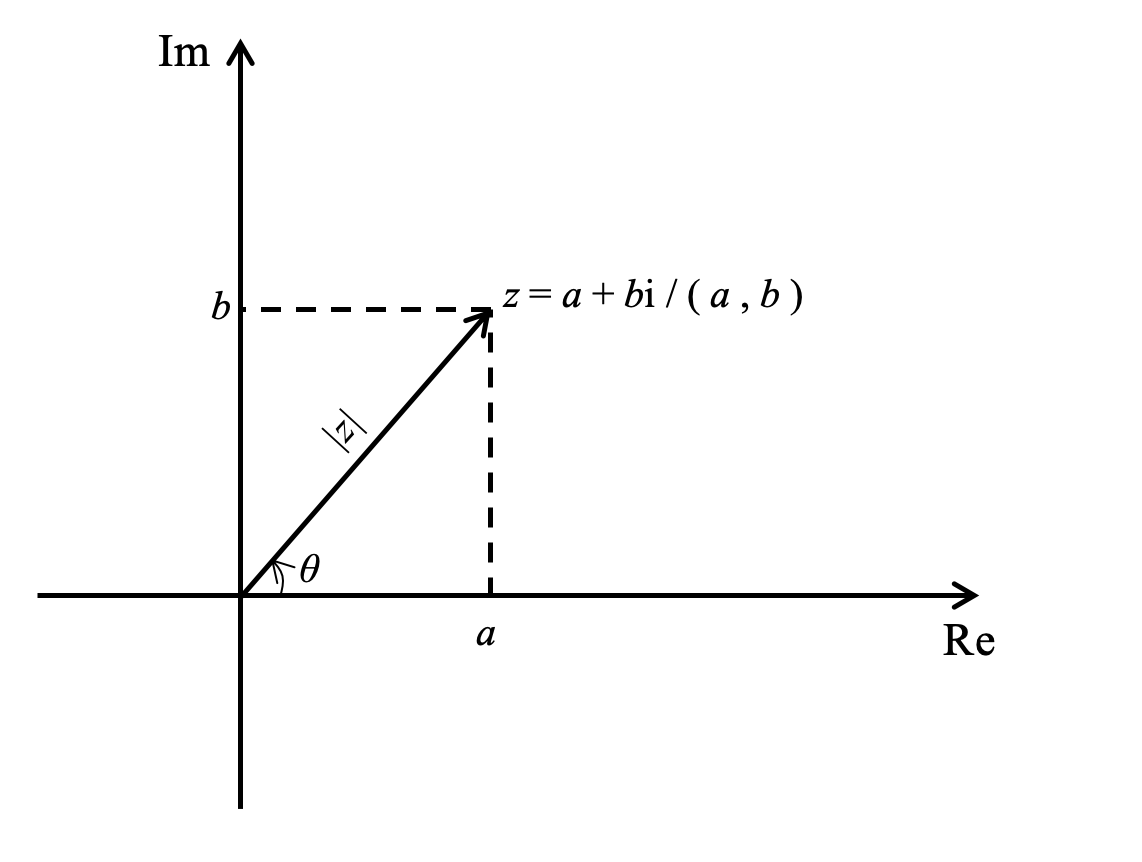
\includegraphics[width=0.5\textwidth]{Fig.1.1.jpg}
  \end{figure}
  $z=a+b\i$ can be represented on a complex plane with real coordinate $a$ and imaginary coordinate $b$. It can also be denoted as $z(a,b)$.
  \begin{itemize}
    \item Modulus of a complex number: 
    $${\color{red}{\left|z\right|=\sqrt{a^2+b^2}}}.$$
    \item Argument of a complex number: 
    $${\color{red}{\Arg(z)=\arctan\left(\frac{b}{a}\right)(+k\pi)}}{\color{green}{\ \rightarrow\ \arctan x\in\left.\right]-\frac{\pi}{2},\frac{\pi}{2}\left[\right.}}.$$
    {\color{green}{*When determine a complex number, first draw it on the plane to show which quadrant it is in.}}\\
    The range of arugment is $\left[0,2\pi\right]$ or $\left[-\pi,\pi\right]$.
    \item Use modulus and argument to express a complex number: 
    $${\color{red}{a=\left|z\right|\cdot\cos\theta}};$$
    $${\color{red}{b=\left|z\right|\cdot\sin\theta}}.$$
  \end{itemize} 
  \item If $z=a+b\i$ and $|z|=1$, then {\color{red}{$z^*=z^{-1}$}}.
  \begin{proof}
    $$\begin{aligned}
      &\because |z|=1\\
      &\therefore \sqrt{a^2+b^2}=1\\
      &\therefore a^2+b^2=1
    \end{aligned}$$
    \begin{multicols}{2}
    \begin{boxed}{\text{Method 1}}\end{boxed}
    $$\begin{aligned}
      \text{RHS}=z^{-1}&=\frac{1}{a+b\i}=\frac{a-b\i}{(a+b\i)(a-b\i)}\\
      &=\frac{a-b\i}{a^2+b^2}=a-b\i\\
      &=z^*=\text{LHS}.
    \end{aligned}$$
    \begin{boxed}{\text{Method 2}}\end{boxed}
    $$\begin{aligned}
      z\cdot z^*&=(a+b\i)(a-b\i)\\
      &=a^2+b^2\\
      &=|z|^2=1\\
      \therefore \ &\ z^*=z^{-1}
    \end{aligned}$$
    \end{multicols}
  \end{proof}
  \item When $|z|\neq 1$, {\color{red}{$z^*=\frac{|z|^2}{z}$}}, and {\color{red}{$z^{-1}=\frac{z^*}{|z|^2}$}}.
  \item Properties of modulus and arguments: \\
  For complex number $s$ and $t$ $\in\C$: 
  \begin{itemize}
    \item $$|st|=|s||t|$$
    \item $$\left|\frac{s}{t}\right|=\frac{|s|}{|t|}$$
    \item $$\Arg(st)=\Arg(s)+\Arg(t)+2k\pi$$
    \item $$\Arg\left(\frac{s}{t}\right)=\Arg(s)-\Arg(t)+2k\pi$$
  \end{itemize}
\end{enumerate}

\subsubsection{Complex Number in Other Forms}
\begin{enumerate}
  \item The Polar Form (Modulus-Argument Form): 
  \begin{itemize}
    \item $${\color{red}{z=r(\cos\theta+\i\sin\theta)=r\cis\theta}}$$
    \begin{proof}
      According to the Argand Diagram: 
      $$z=x+y\i=r\cos\theta+\i r\sin\theta=r(\cos\theta+\i\sin\theta).$$
    \end{proof}
    \item $${\color{red}{z_1z_2=r_1r_2\cis(\theta_1+\theta_2)}}$$
    \item $${\color{red}{\frac{z_1}{z_2}=\frac{r_1}{r_2}\cis(\theta_1-\theta_2)}}$$
  \end{itemize}
  \item de Movrie's Theorem: 
  \begin{itemize}
    \item By Maclaurin Series: $${\color{red}{e^{\i\theta}=\cis\theta}}=\cos\theta+\i\sin\theta.$$
    \item Exponential form of complex number: 
    $${\color{red}{z=re^{\i\theta}=r\cis\theta}}.$$
  \end{itemize}
  \item Cartesian Form: Addition and Substraction\\
  Modulus-Argument Form: Multiply and Division\\
  Exponential Form: Exponents and Roots
  \item Since $\cis\theta=\cis(\theta+2k\pi),$ 
  $${\color{red}{re^{\i\theta}=re^{\i(\theta+2k\pi)}}}.$$
  \begin{example}
    \textbf{Find $e^{\i\frac{17\pi}{12}}$ in the form of Cartesian.}
    $$\begin{aligned}
      e^{\i\frac{17\pi}{12}}=e^{\i\left(\frac{7\pi}{6}+\frac{\pi}{4}\right)}&=e^{\i\frac{7\pi}{6}}\cdot e^{\frac{\pi}{4}}\\
      &=\cis\left(\frac{7\pi}{6}\right)\cdot\cis\left(\frac{\pi}{4}\right)\\
      &=\left(-\frac{\sqrt{3}}{2}-\frac{1}{2}\i\right)\left(\frac{\sqrt{2}}{2}+\frac{\sqrt{2}}{2}\i\right)=\frac{\sqrt{2}-\sqrt{6}}{4}-\frac{\sqrt{2}+\sqrt{6}}{4}\i.
    \end{aligned}$$
  \end{example}
\end{enumerate}

\subsubsection{Power of Complex Number}
\begin{enumerate}
  \item For a complex number $z=re^{\i\theta},$
  $${\color{red}{z^n=r^ne^{\i n\theta}}}.$$
  \begin{example}
    \textbf{Find $\left(3\cos\frac{2\pi}{3}-3\i\sin\frac{\pi}{3}\right)^3$}
    $$\begin{aligned}
      \left(3\cos\frac{2\pi}{3}-3\i\sin\frac{\pi}{3}\right)^3&=\left(-3\cos\frac{\pi}{3}-3\i\sin\frac{\pi}{3}\right)^3\\
      &=\left(-3\left(\cos\frac{\pi}{3}+\i\sin\frac{\pi}{3}\right)\right)^3\\
      &=(-3)^3(e^{\i\frac{\pi}{3}})^3\\
      &=-27e^{\i\pi}\\
      &=-27(-1)=27.
    \end{aligned}$$
    {\color{green}{Key learnings: \\
    1. $z=3$ is only the fundemental root of equation $z^3=27$. In $\C$, there are other two complex roots that satisfy the euqation.\\
    2. In $\C$, $\sqrt{4}=\pm 2=2+0\cdot\i\text{ or }-2+0\cdot\i$.}}
  \end{example}
  \begin{example}
    \textbf{Given a complex number $\omega\neq 1$ is one of the solutions of $z^3=1.$\\
    a. Prove $\omega^2+\omega+1=0$;\\
    b. Calculate $\omega^{2019}+\omega^{2020}+\omega^{2021}+\omega^{2022}$.}
    \begin{enumerate}
      \item \begin{boxed}{\text{Approach A}}\end{boxed}
      $$\begin{aligned}
        &\because \omega^3=1\\
        &\therefore \omega^3-1=0\ \Rightarrow\ (\omega-1)(\omega^2+\omega+1)=0\\
        &\because \omega\neq 1\\
        &\therefore \omega^2+\omega+1=0.
      \end{aligned}$$
      \begin{boxed}{\text{Approach B}}\end{boxed}
      $\omega^2+\omega+1=0$ is a geometric sequence, $u_1=1,\ r=\omega:$
      $$S_3=\frac{u_1(1-r^3)}{1-r}=\frac{1-\omega^3}{1-\omega}=\frac{0}{1-\omega}=0.$$
      \item $$\begin{aligned}
        \omega^{2019}+\omega^{2020}+\omega^{2021}+\omega^{2022}&=\omega^{2019}\times(1+\omega+\omega^2+\omega^3)\\
        &=\omega^{2019}(0+1)=\omega^{2019}\\
        &=\left(\omega^{3}\right)^{673}=1.
      \end{aligned}$$
    \end{enumerate}
  \end{example}
  \begin{example}
    \textbf{Find: \\
    a. $1^\i$;\\
    b. $\ln(-1)$;\\
    c. $\ln(-c)$, where $c$ is a constant. }
    \begin{enumerate}
      \item $$1=e^{\i 2\pi}\ \Rightarrow\ 1^\i=\left(e^{\i 2\pi}\right)^\i=e^{-2\pi}. \ \ \ \ {\color{green}{(1^\i=e^{-2k\pi}, k\in\Z)}}$$
      \item $$-1=e^{\i\pi}\ \Rightarrow\ \ln(-1)=\ln\left(e^{\i\pi}\right)=\i\pi.$$
      \item $$\ln(-c)=\ln\left[(-1)\cdot c\right]=\ln(-1)+\ln(c)=\ln(c)+\i\pi.$$
    \end{enumerate}
  \end{example}
\end{enumerate}

\subsubsection{Polynomial Function with Complex Roots}
\begin{enumerate}
  \item Conjugate Pair Theorem: 
  \begin{theorem}
    If $z$ is a complex root of $P(x)$, then the conjugate of $z(z^*)$ is also a complex root of $P(x)$. ($P(x)$ should be a polynomial with {\color{red}{rational}} coefficients.)
  \end{theorem}
  \item Properties of Conjugate. 
  \begin{itemize}
    \item $$(s\pm t)^*=s^*\pm t^*$$
    \item $$(st)^*=s^*t^*$$
    \item $$\left(\frac{s}{t}\right)^*=\frac{s^*}{t^*}$$
  \end{itemize}
\end{enumerate}

\subsubsection{Root of Complex Numbers}
\begin{enumerate}
  \item The Root of Unity: 
  \begin{theorem}
    For any complex equation $\omega^n=1$, there are $n$ distinct roots: 
    $$1=e^{\i(0+2k\pi)}=\omega^n,\ k\in\Z\ \ \ \ \Rightarrow\ \ \ \ \omega=e^{\i\frac{2k\pi}{n}},\ k\in\Z.$$
  \end{theorem}
  \begin{example}
    \textbf{Solve $z^3=8$.}
    $$\begin{aligned}
      z^3=8\cdot 1=8e^{i(0+2k\pi)}\ &\ \Rightarrow\ \ z=2e^{i\frac{2k\pi}{3}},\ k\in\Z\\
      k&=0:\ z=2\\
      k&=1:\ z=2e^{i\frac{2\pi}{3}}=2\cis\left(\frac{2\pi}{3}\right)=-1+\sqrt{3}\i\\
      k&=2:\ z=2e^{i\frac{4\pi}{3}}=2\cis\left(\frac{4\pi}{3}\right)=-1-\sqrt{3}\i
    \end{aligned}$$
  \end{example}
  \item Property of $\cis\theta$: 
  $$\cis(-\theta)=\cos\theta-\i\sin\theta$$
  \begin{proof}
    $$\begin{aligned}
      \cos\theta-\i\sin\theta&=\cos(-\theta)+\i\sin(-\theta)\\
      &=\cis(-\theta).
    \end{aligned}$$
  \end{proof}
\end{enumerate}

\newpage
\section{Topic 2 Functions}
\subsection{Foundations of Functions}
\begin{enumerate}
    \item Relations and functions: 
    \begin{definition}
        A \textbf{\color{red}{relation}} $R$ is a set of ordered pairs $(x,y)$ such that $x\in A,\ y\in B$, and sets $A,\ B$ are not empty. 
    \end{definition}
    \begin{definition}
        A \textbf{\color{red}{function}} $f$ is a relation in which every $x$-value has a unique $y$-value. 
    \end{definition}
    \item Domain and Range: 
    \begin{definition}
        \textbf{\color{red}{Domain}} is the set of $x$-values. 
    \end{definition}
    \begin{definition}
        \textbf{\color{red}{Range}} is the set of $y$-values. 
    \end{definition}
    \begin{itemize}
        \item Domain and Range should be in inverval notation. 
        \begin{enumerate}
            \item Using invervals to express the inequalities
            \begin{example}
                $$\left[\right.3,4\left[\right. \text{ means }3\leq x<4$$
            \end{example}
            \item If the interval will be joint, we use ${\color{red}{\cup}}$ to join the inverval. 
            \begin{example}
                $$3<x<4\text{ or }x\geq 5\ \Rightarrow\ \left.\right]3,4\left.\right]\cup\left[5,+\infty\right.\left[\right.$$
            \end{example}
            \begin{example}
                \textbf{Find the interval notation for the domain of $\displaystyle f(x)=\frac{1}{x}$.}
                $$x\in\left.\right]-\infty,0\left[\right.\cup\left.\right]0,+\infty\left[\right.\text{ OR } x\in\R\setminus 0$$
                {\color{green}{Note: $\setminus$ means "exclude."}}
            \end{example}
        \end{enumerate}
        \item Since the $y$-values (outputs) depend on the $x$-values (inputs), $y$ is the \textbf{\color{red}{dependent variable}}, and $x$ is the \textbf{\color{red}{independent variable}}.
        \item The independent vairbale $x$ is also called the \textbf{\color{red}{argument}} of the function. 
    \end{itemize}
    \item Vertical Line test: 
    \begin{itemize}
        \item To test whether a relation is a function. 
        \item Since every $x$ has one and only one value of $y$, there should be only one intersects. 
    \end{itemize}
    \item Inverse of a function: 
    \begin{definition}
        $f^{-1}(x)$ is the \textbf{\color{red}{inverse function}} of $f(x)$.
        \begin{figure}[H]
            \centering
            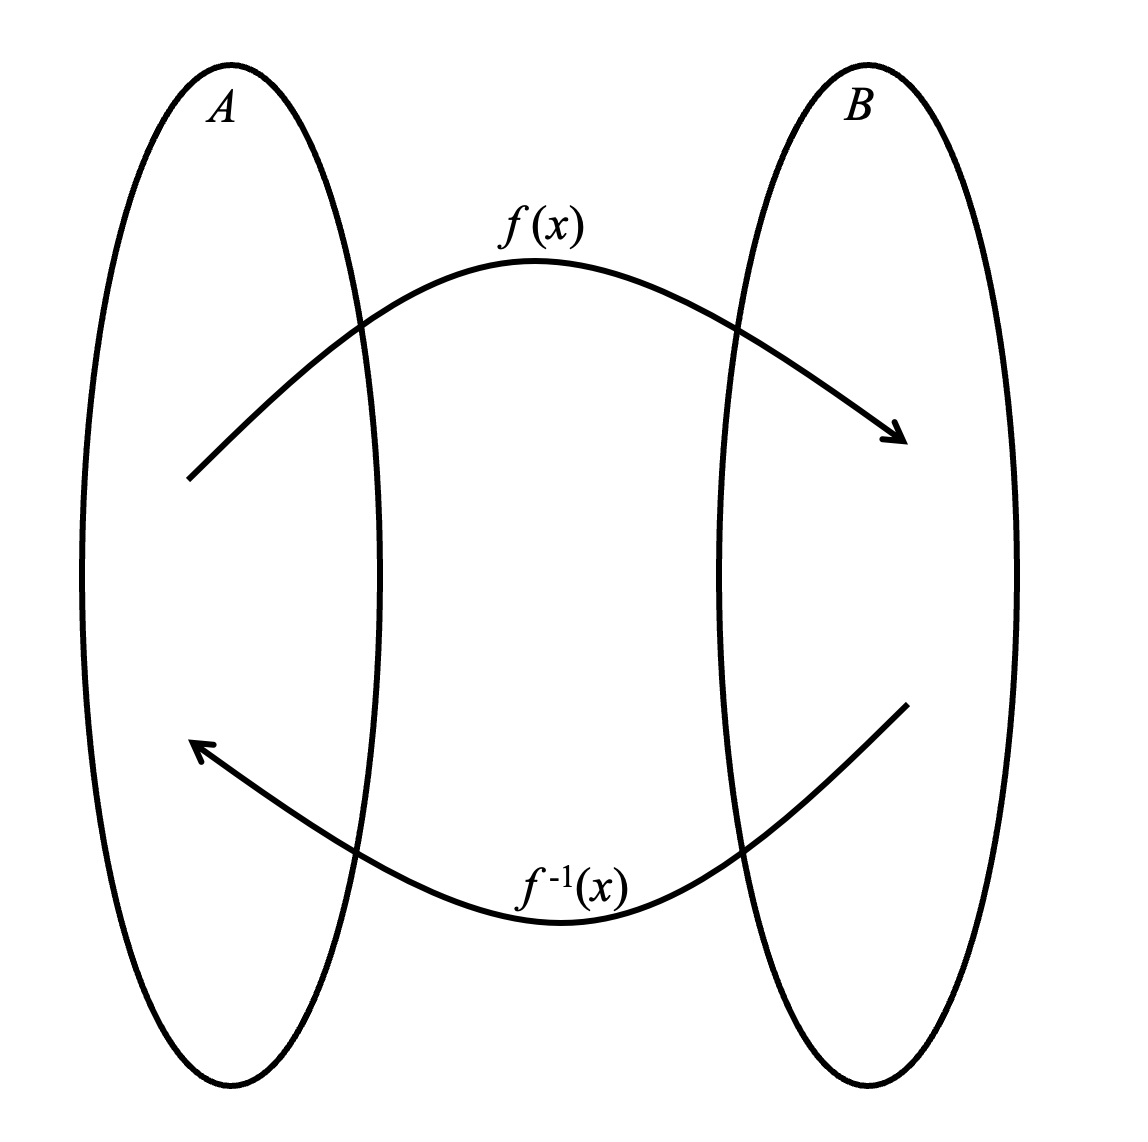
\includegraphics[width=0.5\textwidth]{Fig.2.1.jpg}
          \end{figure}
    \end{definition}
    \begin{example}
        $f(1)=3\ \Rightarrow\ f^{-1}(3)=1;\ f(x)=x+5\ \Rightarrow\ f^{-1}(x)=x-5$
    \end{example}
    \begin{itemize}
        \item In inverse function, the input becomes the output, the output becomes the input. 
        \item In inverse function, the domain becomes the range, the range becomes the domain. 
        \begin{example}
            \begin{enumerate}
                \item \textbf{Find the inverse function of $\displaystyle y=\frac{x+2}{3}$.}
                $$\begin{aligned}
                    3y=x+2&\Rightarrow x=3y-2\\
                    f^{-1}(x)&=3x-2
                \end{aligned}$$
                \item \textbf{Find the inverse function of $f(x)=\displaystyle \frac{x}{x+1}$.}
                $$\begin{aligned}
                    y=\frac{x}{x+1}\Rightarrow xy+y=x&\Rightarrow xy+x=y\\
                    \therefore y(x-1)=-x&\Rightarrow y=-\frac{x}{x-1}
                \end{aligned}$$
                \item \textbf{Find the inverse of $\{.(4,2),(0,2),(-2,2)\}$}
                $$\text{Inverse: }\{(2,4),(2,0),(2,-2)\}$$
            \end{enumerate}
        \end{example}
        \item By restricting the domain, we can find $f^{-1}(x)$ of $f(x)$, if the direct inverse of $f(x)$ is not a function.
        \begin{example}
            \begin{figure}[H]
                \centering
                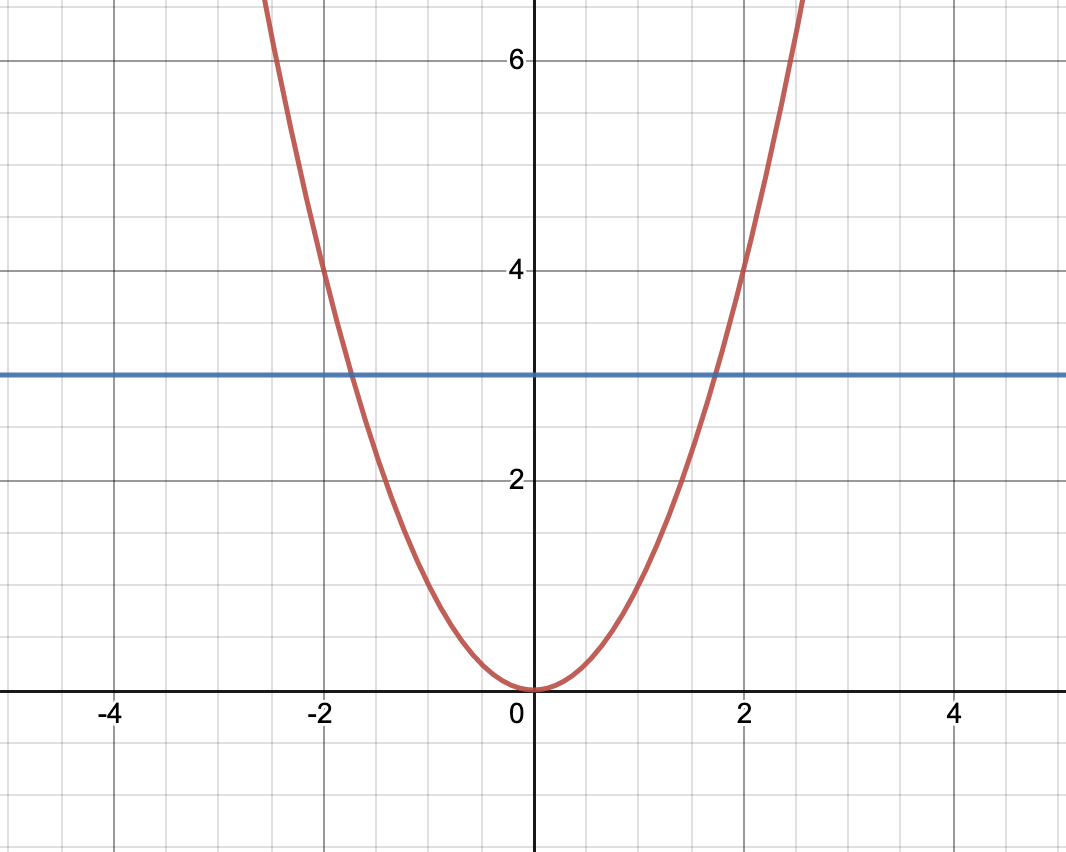
\includegraphics[width=0.5\textwidth]{Fig.2.2.jpg}
              \end{figure}
              {\color{red}{Horizontal line test}}: The largest domain we can find $f^{-1}(x)$ is $x\leq 0$ or $x>0$.
        \end{example} 
    \end{itemize}
    \item Composite Functions: 
    \begin{definition}
        We use {\color{red}$(g\circ h)(x)$} or {\color{red}{$g(h(x))$}} to represent composite functions. 
        \begin{figure}[H]
            \centering
            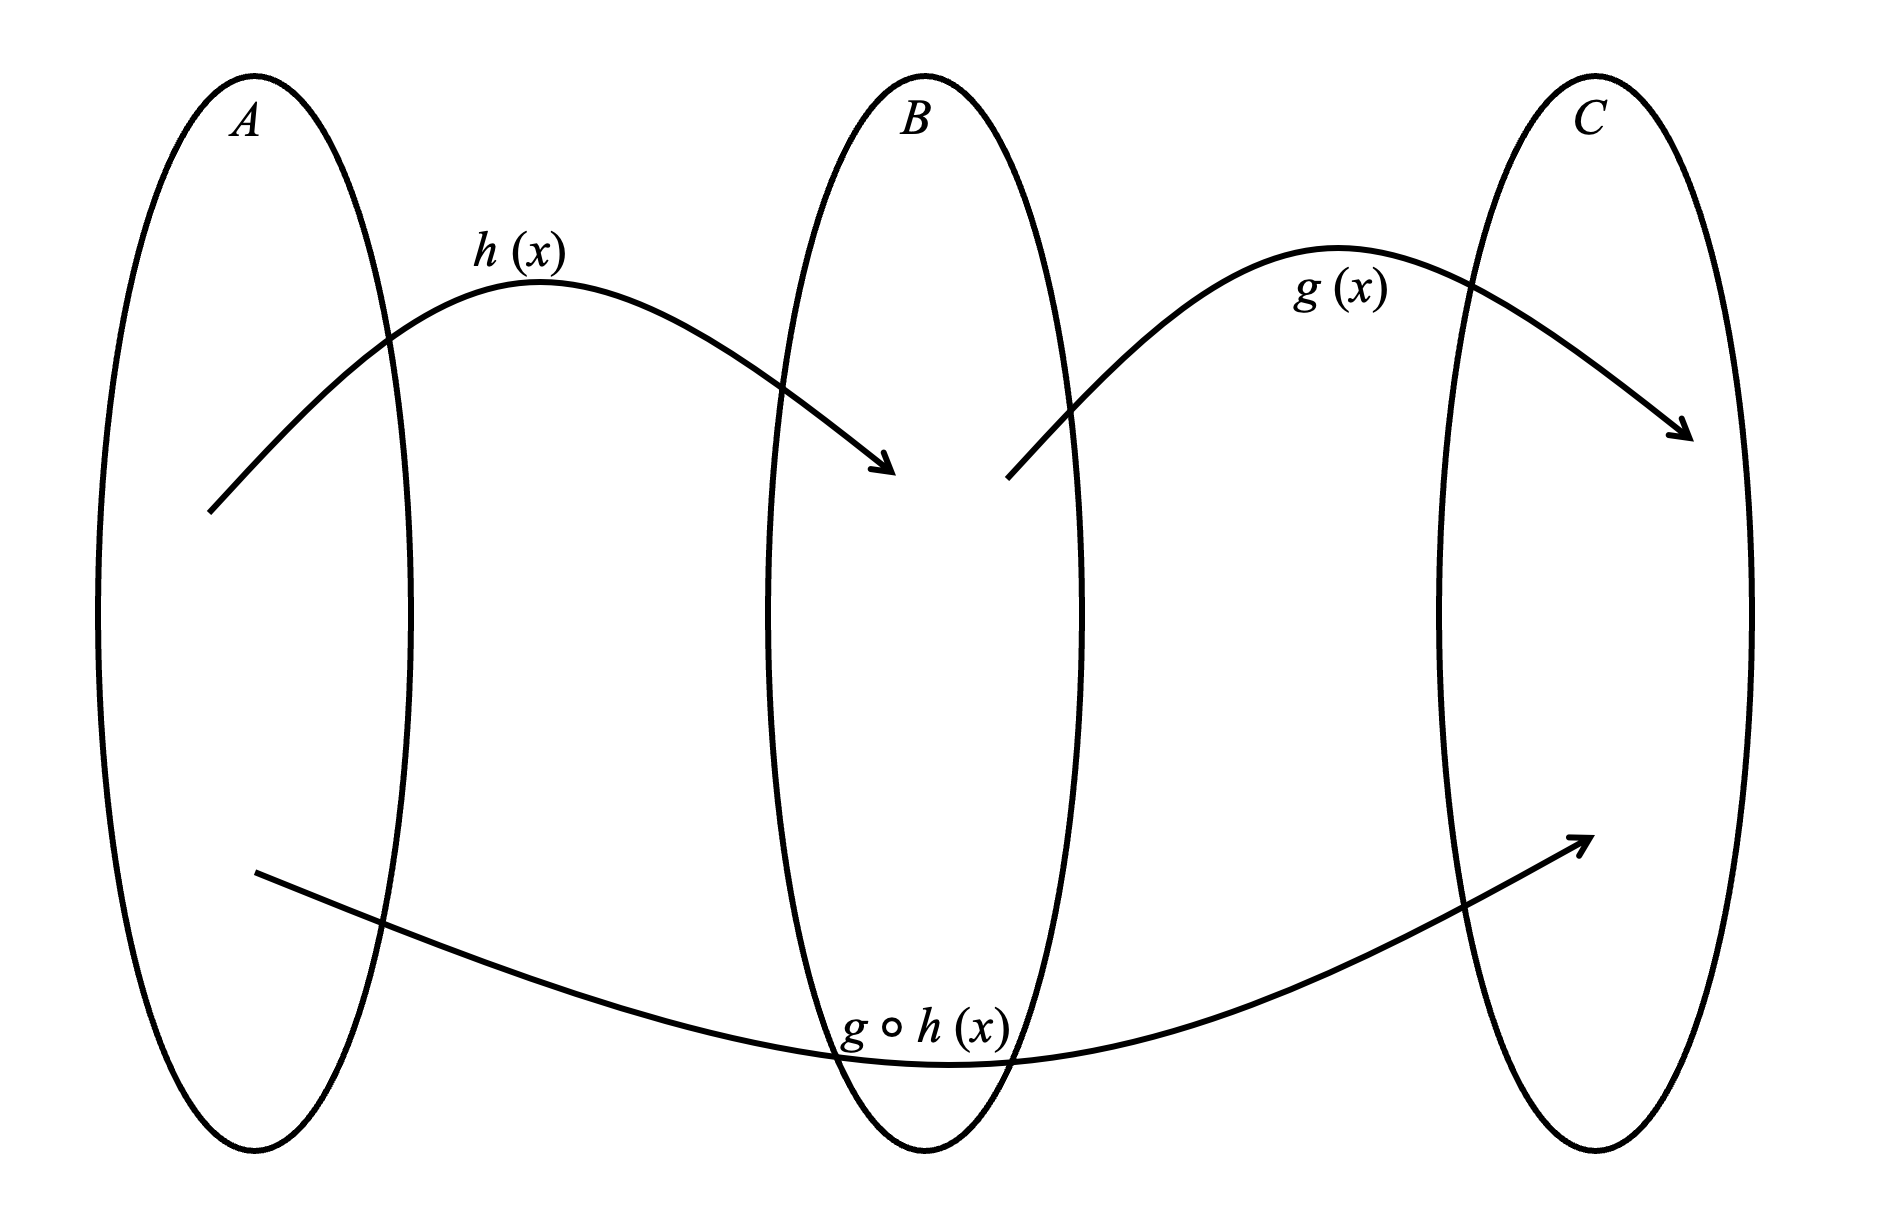
\includegraphics[width=0.7\textwidth]{Fig.2.3.jpg}
          \end{figure}
    \end{definition}
    \begin{example}
        \textbf{Given $f:x\mapsto  3x-6,\ g:x\mapsto\displaystyle\frac{1}{3}x+2$. Find $(f\circ g)(x)$ and $(g\circ f)(x)$.}
        $$(f\circ g)(x)=f\left(g(x)\right)=3(\frac{1}{3}x+2)-6=x.$$
        $$(g\circ f)(x)=g\left(f(x)\right)=\frac{1}{3}(3x-6)+2=x.$$
    \end{example}
    When $f$ and $g$ are inverse functions: $${\color{red}{(f\circ g)(x)(x)=x=(g\circ f)(x)}}.$$
    \item $f(x)$ and $f^{-1}(x)$ are symmetrical to $y=x$ since $D_f=R_{f^{-1}}$, $R_f=D_{f^{-1}}$. That is, {\color{red}{if $f(x)$ passes through $(a,b)$, $f^{-1}(x)$ passes through $(b,a)$}}.
\end{enumerate}

\subsection{Quadratic Functions}
\begin{enumerate}
    \item The Standard Form: 
    $$\color{red}{y=ax^2+bx+c},$$
    where $a$ is the coefficient of $x^2$, $b$ is the coefficient of x, and $c$ is the constant or $y$-intercept. $a,b,c\neq 0$. 
    \begin{itemize}
        \item Zeros of the function ($x$-intercepts): 
        $$\color{red}{x=\frac{-b\pm\sqrt{b^2-4ac}}{2a}},$$
        where $\Delta=b^2-4ac$ is the discriminant of the function. 
        \item Euqation of the line of symmetry \& $x$-coordinate of the vertex
        $$x=-\frac{b}{2a}.$$
        \item Vieta's Formula: 
        \begin{theorem}
            Assume $x_1,\ x_2$ are two roots for equation $ax^2+bx+c=0\ (a\neq 0)$, then
            $$\color{red}x_1+x_2=-\frac{b}{a};$$
            $$\color{red}x_1\cdot x_2=\frac{c}{a}.$$
        \end{theorem}
        \item When $a>0,$ the parabola opens upwards. \\
        When $a<0$, the parabola opens downwards.
    \end{itemize}
    \item Completion of square: 
    $${\color{red}{x^2+px+\left(\frac{p}{2}\right)^2-\left(\frac{p}{2}\right)^2=\left(x+\frac{p}{2}\right)^2-\left(\frac{p}{2}\right)^2}}.$$
    \item The Vertex Form: 
    $${\color{red}{y=a(x-h)^2+k,\text{ where }(h,k)\text{ is the vertex}}}.$$
    \begin{example}
        \textbf{Given that $f(x)=ax^2+bx+c,$ find the axis of symmetry and vertex.}
        $$\begin{aligned}
            f(x)&=a\left(x^2+\frac{b}{a}x\right)+c\\
            &=a\left[x^2+\frac{b}{a}x+\left(\frac{b}{2a}\right)^2\right]+c-\frac{b^2}{4a}\\
            &=a\left(x+\frac{b}{2a}\right)^2+\frac{4ac-b^2}{4a}.
        \end{aligned}$$
        $$\begin{aligned}
            \therefore \text{ axis of symmetry: }&x=-\frac{b}{2a}\\
            \text{vertex: }&\left(-\frac{b}{2a},\frac{4ac-b^2}{4a}\right).
        \end{aligned}$$
    \end{example}
\end{enumerate}

\subsection{Higher Order Polynomial Functions}
\begin{enumerate}
    \item Factor Theorem: 
    \begin{theorem}
        If $(x-a)$ is a factor of a polynomial $P(x)$, then $x=a$ must be a root for $P(x)\ \Rightarrow {\color{red}{P(a)=0}}$.
        \begin{proof}
            Assume the quotient when $P(x)$ is divided by $(x-a)$ is $Q(x)$, then $P(x)=Q(x)\cdot(x-a)$. Then, $P(a)=Q(a)\cdot(a-a)=0$.
        \end{proof}
    \end{theorem}
    \item Long division: solving polynomial equation. 
    \begin{example}
        \textbf{For a cubic function, $P(x)=2x^3+bx^2+cx+d,\ P(1)=P(2)=P(3)=2.$ What is $P(0)$?}\\
        Since $P(1)=P(2)=P(3)=2, Q(1)=Q(2)=Q(3)=0,\text{ where }Q(x)=P(x)-2.$\\
        Thus, $Q(x)=2(x-1)(x-2)(x-3).$
        $$\therefore P(x)=Q(2)+2=2(x-1)(x-2)(x-3)+2.$$
        $$\therefore P(0)=2(-1)(-2)(-3)+2=-10.$$
    \end{example}
    \item Remainder Theorem: 
    \begin{theorem}
        When a polynomial $P(x)$ is divided by $(ax-b)$, the remainder $R$ of this division must be $${\color{red}{P\left(\frac{b}{a}\right)}}.$$
        \begin{proof}
            Assume the quotient is $Q(x)$, and the reminder is $R$: 
            $$P(x)=(ax-b)Q(x)+R.$$
            $$P\left(\frac{b}{a}\right)=0\cdot Q(X)+R=R.$$
        \end{proof}
    \end{theorem}
    \item Roots of Cubic Functions: 
    \begin{theorem}
        For a cubic function $f(x)=ax^3+bx^2+cx+d$, given the roots of it are $\alpha,\ \beta$, and $\gamma$. Then, 
        $${\color{red}{\begin{cases}
            \alpha+\beta+\gamma=-\displaystyle\frac{b}{a}\ \Rightarrow\ \sum\alpha=-\frac{b}{a}\\
            \displaystyle\alpha\beta+\alpha\gamma+\beta\gamma=\frac{c}{a}\ \Rightarrow\ \sum\alpha\beta=\frac{c}{a}\\
            \displaystyle\alpha\beta\gamma=-\frac{d}{a}\ \Rightarrow\ \sum\alpha\beta\gamma=-\frac{d}{a}
        \end{cases}}}$$
        \begin{proof}
            Since $\alpha,\ \beta,\ \gamma$ are roots of $f(x)$, 
            $$f(x)=a(x-\alpha)(x-\beta)(x-\gamma).$$
            $$\text{So } a(x-\alpha)(x-\beta)(x-\gamma)=ax^3+bx^2+cx+d,$$
            $$\text{i.e., }ax^3-a(\alpha+\beta+\gamma)x^2+a(\alpha\beta+\alpha\gamma+\beta\gamma)x-a\alpha\beta\gamma=ax^3+bx^2+cx+d.$$
            $$\Rightarrow\ \alpha+\beta+\gamma=-\frac{b}{a}, \alpha\beta+\alpha\gamma+\beta\gamma=\frac{c}{a}, \alpha\beta\gamma=-\frac{d}{a}.$$
        \end{proof}
        \begin{theorem}
            $$\sum\alpha=-\frac{b}{a},\ \sum\alpha\beta=\frac{c}{a},\ \sum\alpha\beta\gamma=-\frac{d}{a},\ \sum\alpha\beta\gamma\delta=\frac{e}{a}.$$
        \end{theorem}
    \end{theorem}
\end{enumerate}

\subsection{Rational Functions}
\begin{enumerate}
    \item Reciprocal Functions: $f(x)=\displaystyle \frac{1}{x}$.
    \begin{itemize}
        \item Domain: $x\in\R,\ x\neq 0$
        \item As $x$ increases, $\displaystyle\frac{1}{x}$ decreases $\Rightarrow x\rightarrow\infty, \displaystyle\frac{1}{x}\rightarrow 0$.
        \item Range: $y\in\R,\ y\neq 0$
        \item \textbf{\color{red}{Asymptotes}}: $x=0$, $y=0$. 
        \item Axis of symmetry: $y=x$, $y=-x$.
        \item \textbf{\color{red}{Self-inversing function}}: have axis of symmetry $y=x$. $$f(x)=f^{-1}(x).$$
    \end{itemize}
    \item $\displaystyle y=\frac{a}{bx+c}$
    \begin{itemize}
        \item Vertical asymptotes (V.A.): $bx+c=0$
        \item Horizontal asymptotes (H.A.): $y=0$
        \begin{example}
            \textbf{Draw the diagram of $\displaystyle y=\frac{5}{3x-1}$.}\\
            $x$-intercept: $0=\frac{5}{3x-1}\Rightarrow$ no solution, no intercept.\\
            H.A.: $y=0$\\
            $y$-intercept: $y=-5$\\
            V.A.: $3x-1=0,\ x=\displaystyle\frac{1}{3}$
            \begin{figure}[H]
                \centering
                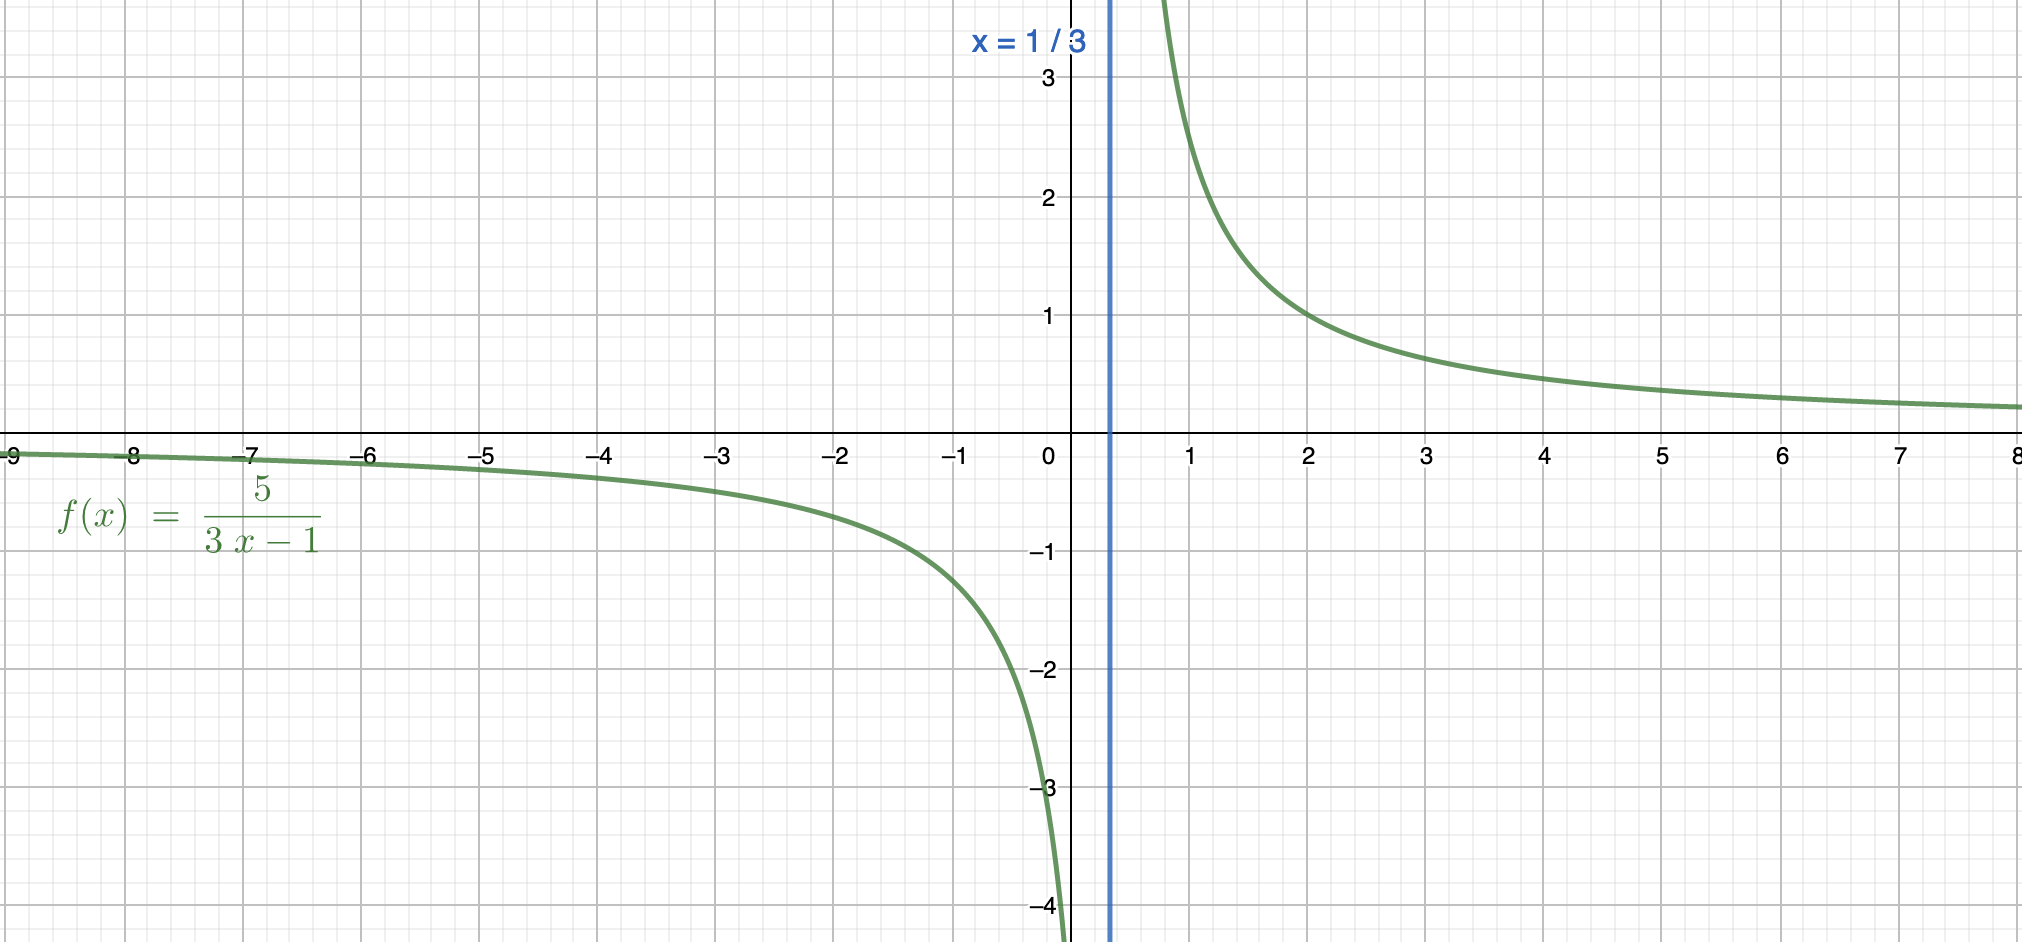
\includegraphics[width=0.8\textwidth]{Fig.2.4.jpg}
            \end{figure}
        \end{example}
    \end{itemize}
    \item $\displaystyle y=\frac{ax+b}{cx+d}$
    \begin{itemize}
        \item V.A.: $cx+d=0$
        \item H.A.: $y=\displaystyle\frac{a}{c}$
    \end{itemize}
    \item $\displaystyle y=\frac{ax+b}{cx^2+dx+e}$
    \begin{itemize}
        \item V.A.: $cx^2+dx+e=0$
        \item H.A.: As $\displaystyle x\to\pm\infty,\ \frac{ax}{cx^2}\to 0$, $y=0$
        \item Intercepts: $\displaystyle\left(0,\frac{e}{c}\right),\ \left(-\frac{e}{d},0\right)$
        \begin{example}
            \textbf{Draw the diagram of $\displaystyle y=\frac{2x-6}{x^2-3x-4}$.}\\
            Intercept: $\displaystyle\left(0,\frac{3}{2}\right),\ \left(3,0\right)$\\
            H.A.: $y=0$\\
            V.A.: $x=-1,\ x=4$
            \begin{figure}[H]
                \centering
                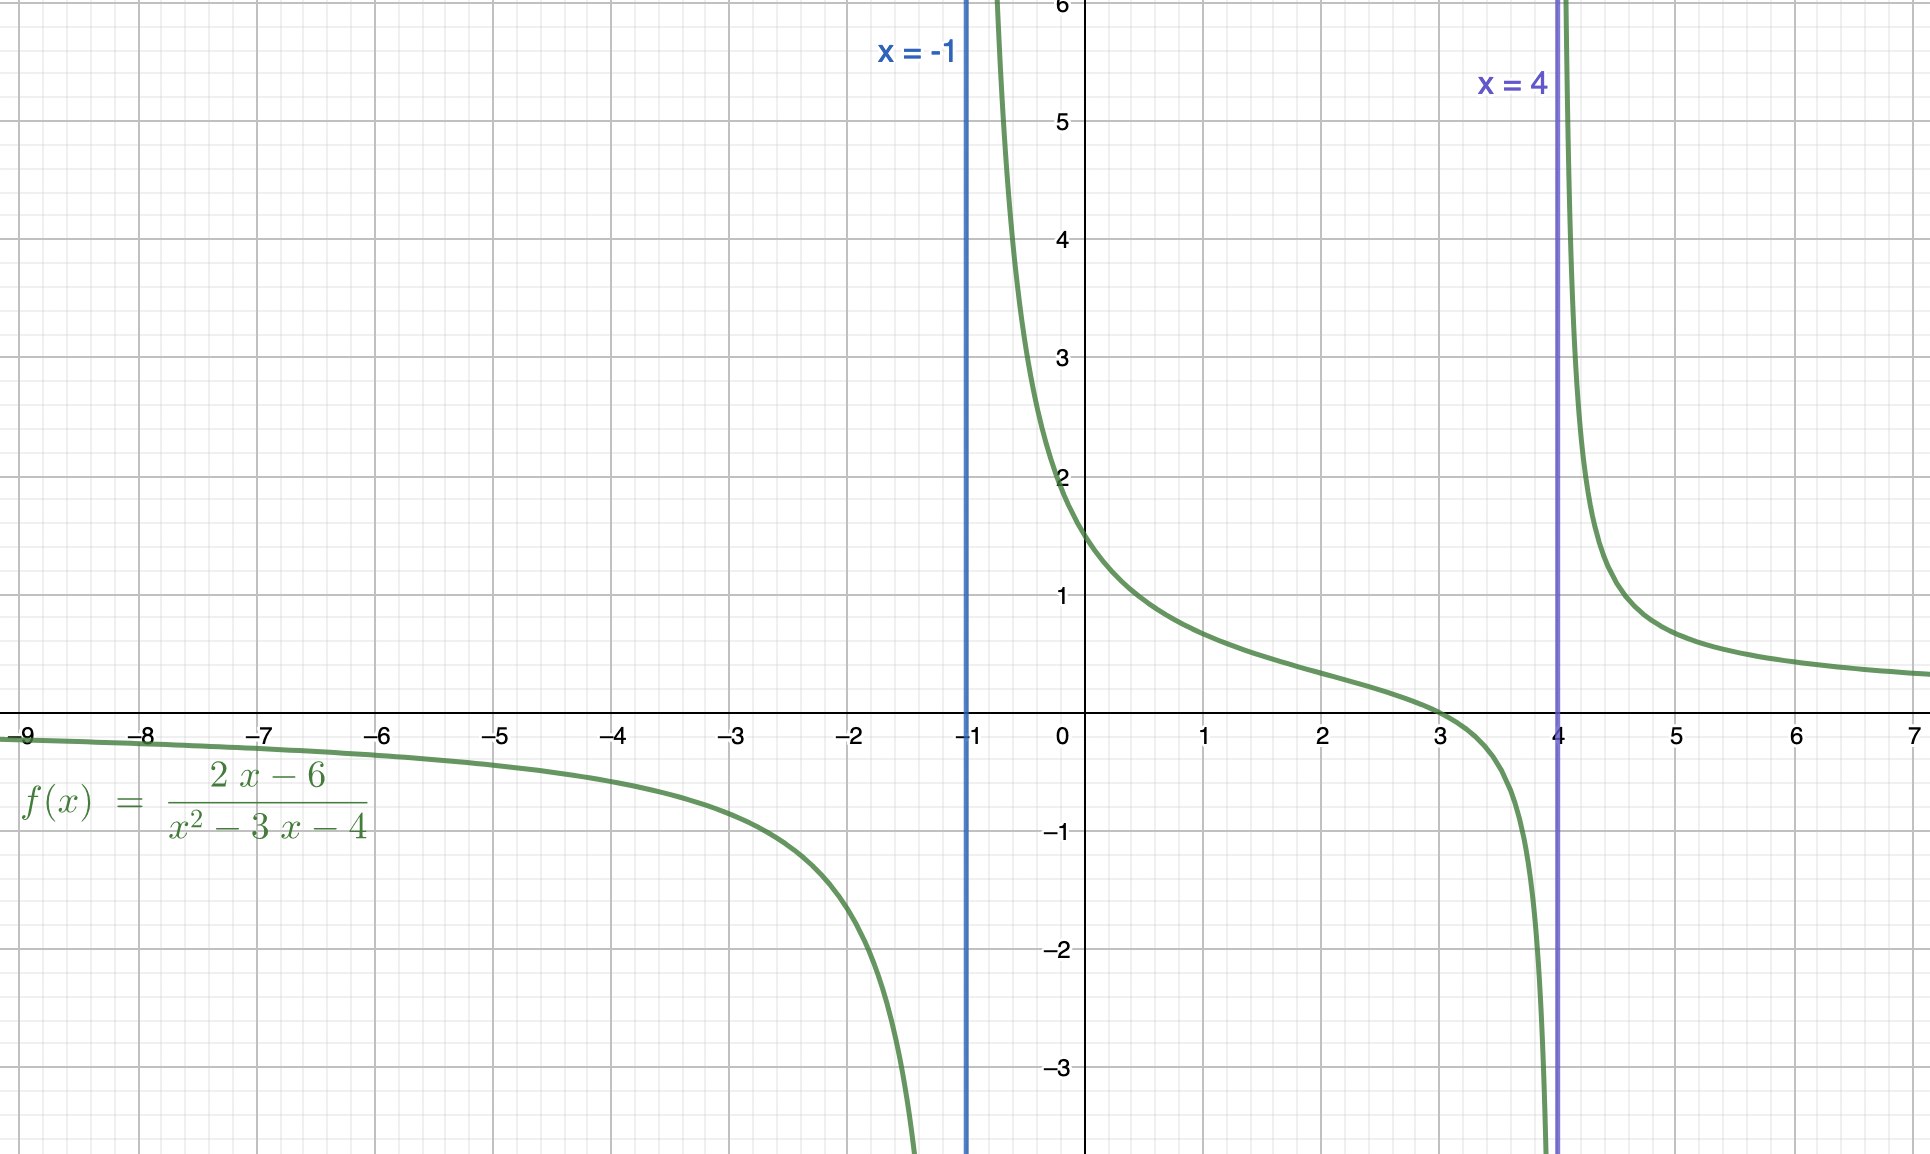
\includegraphics[width=0.8\textwidth]{Fig.2.5.jpg}
            \end{figure}
        \end{example}
        \begin{example}
            \textbf{Draw the diagram of $\displaystyle y=\frac{3x+6}{x^2+2x+1}$.}\\
            Intercept: $\displaystyle\left(0,6\right),\ \left(-2,0\right)$\\
            H.A.: $y=0$\\
            V.A.: $x=-1$
            \begin{figure}[H]
                \centering
                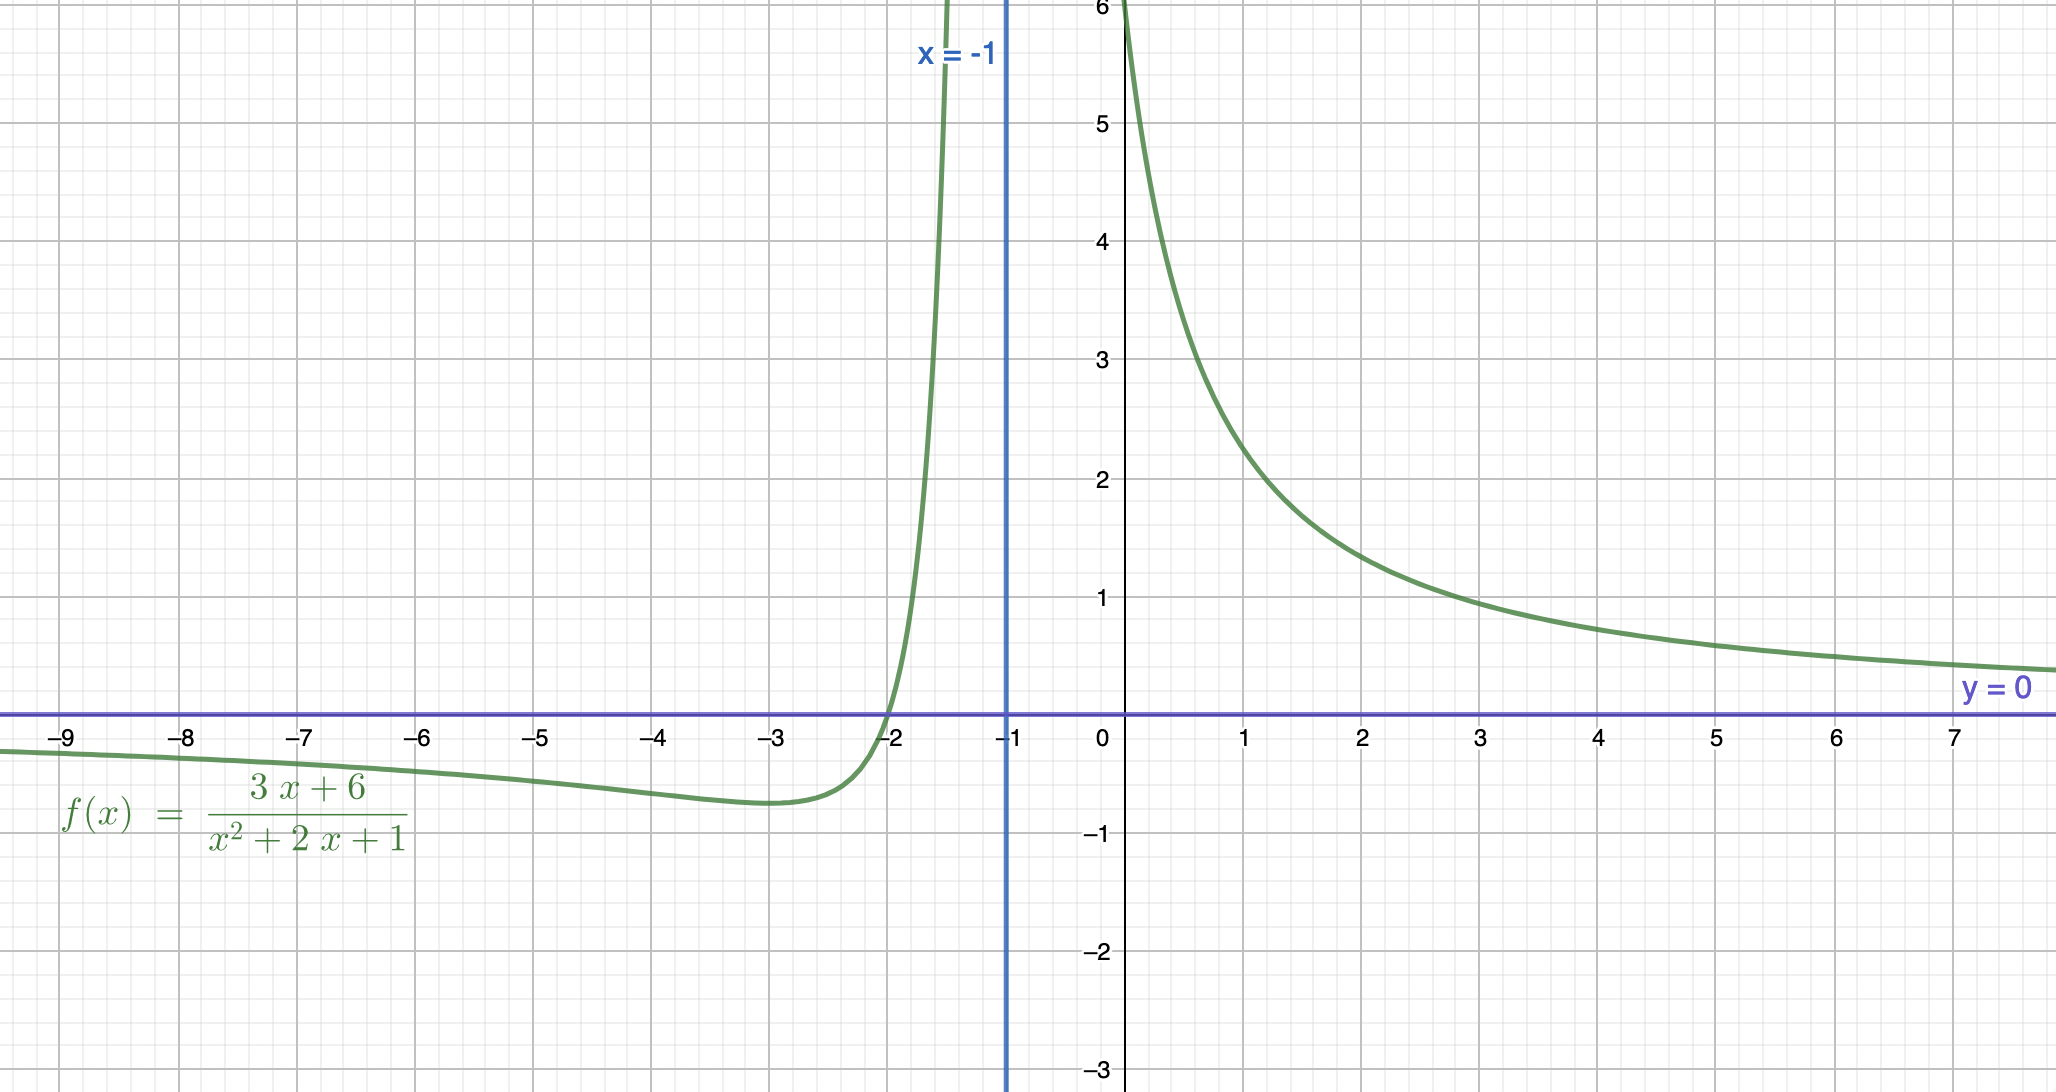
\includegraphics[width=0.8\textwidth]{Fig.2.6.jpg}
            \end{figure}
        \end{example}
        \begin{example}
            \textbf{Draw the diagram of $\displaystyle y=\frac{x-6}{x^2+2x+3}$.}\\
            Intercept: $\displaystyle\left(6,0\right),\ \left(0,-2\right)$\\
            When $x\to\infty,\ f(x)$ is positive. When $x\to -\infty,\ f(x)$ is negative. 
            \begin{figure}[H]
                \centering
                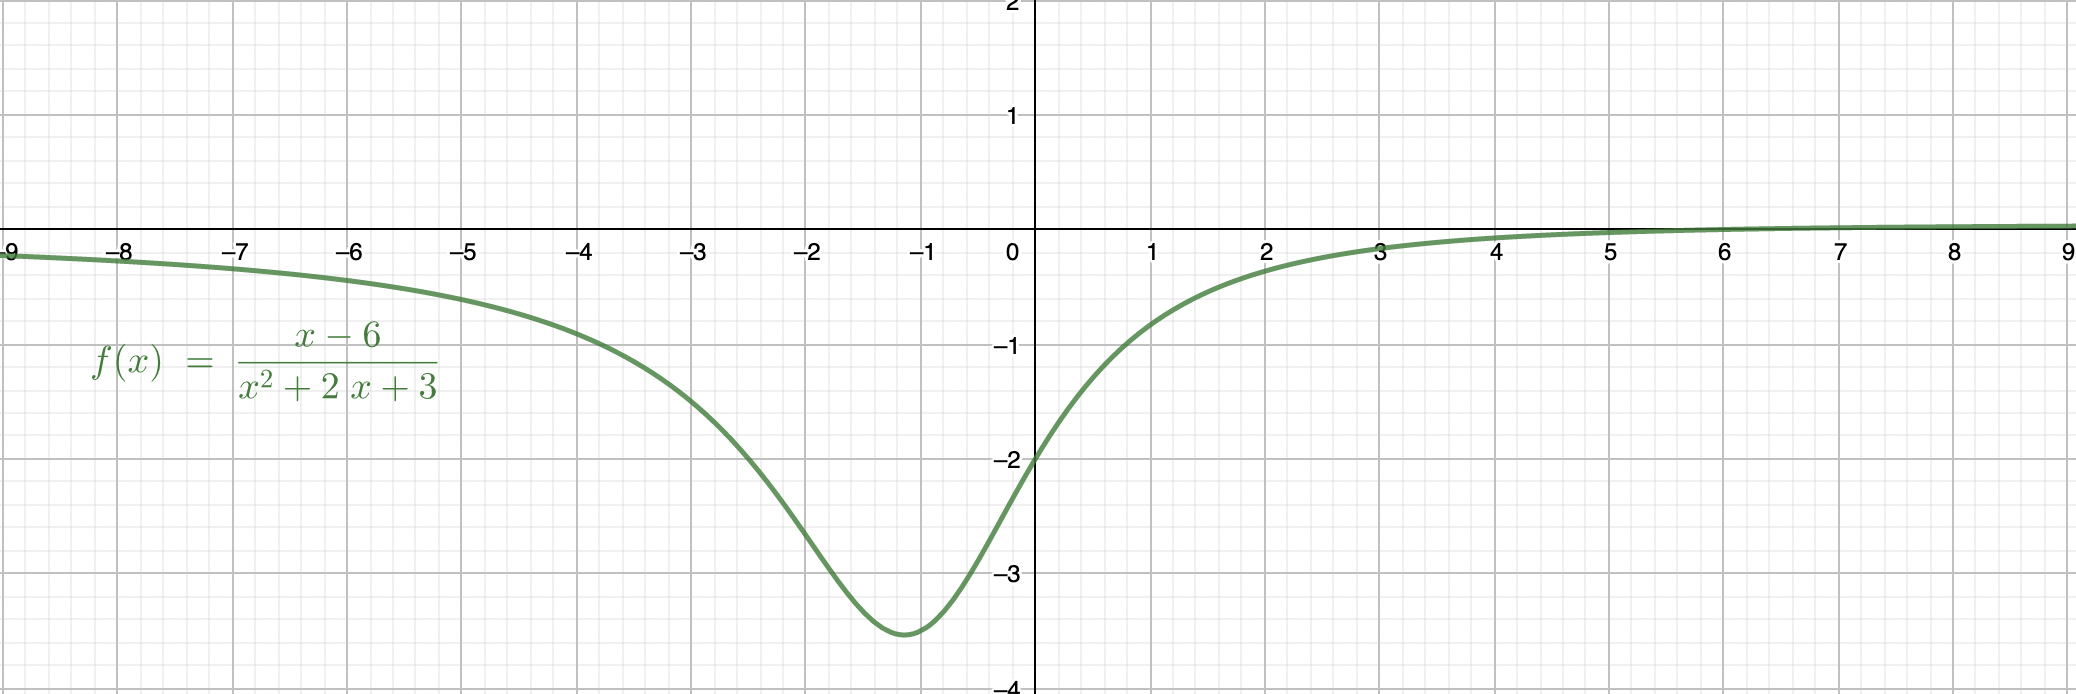
\includegraphics[width=0.8\textwidth]{Fig.2.7.jpg}
            \end{figure}
        \end{example}
    \end{itemize}
    \item $\displaystyle y=\frac{ax^2+bx+c}{dx+e}$
    \begin{itemize}
        \item V.A.: $dx+e=0$
        \item \textbf{\color{red}{Oblique Asymptote}}: Quotient of $(ax^2+bx+c)$ dividied by $(dx+e)$.
        \item Intercepts: $\displaystyle \left(0, \frac{c}{e}\right),\ ax^2+bx+c=0$
        \begin{example}
            \textbf{Draw the diagram of $\displaystyle y=\frac{x^2+3x+2}{x-2}$.}\\
            Intercept: $\displaystyle\left(0,-1\right),\ \left(-1,0\right),\ \left(-2,0\right)$\\
            V.A.: $x=2$\\
            O.A.: $y=x+5$ (Use long division)
            \begin{figure}[H]
                \centering
                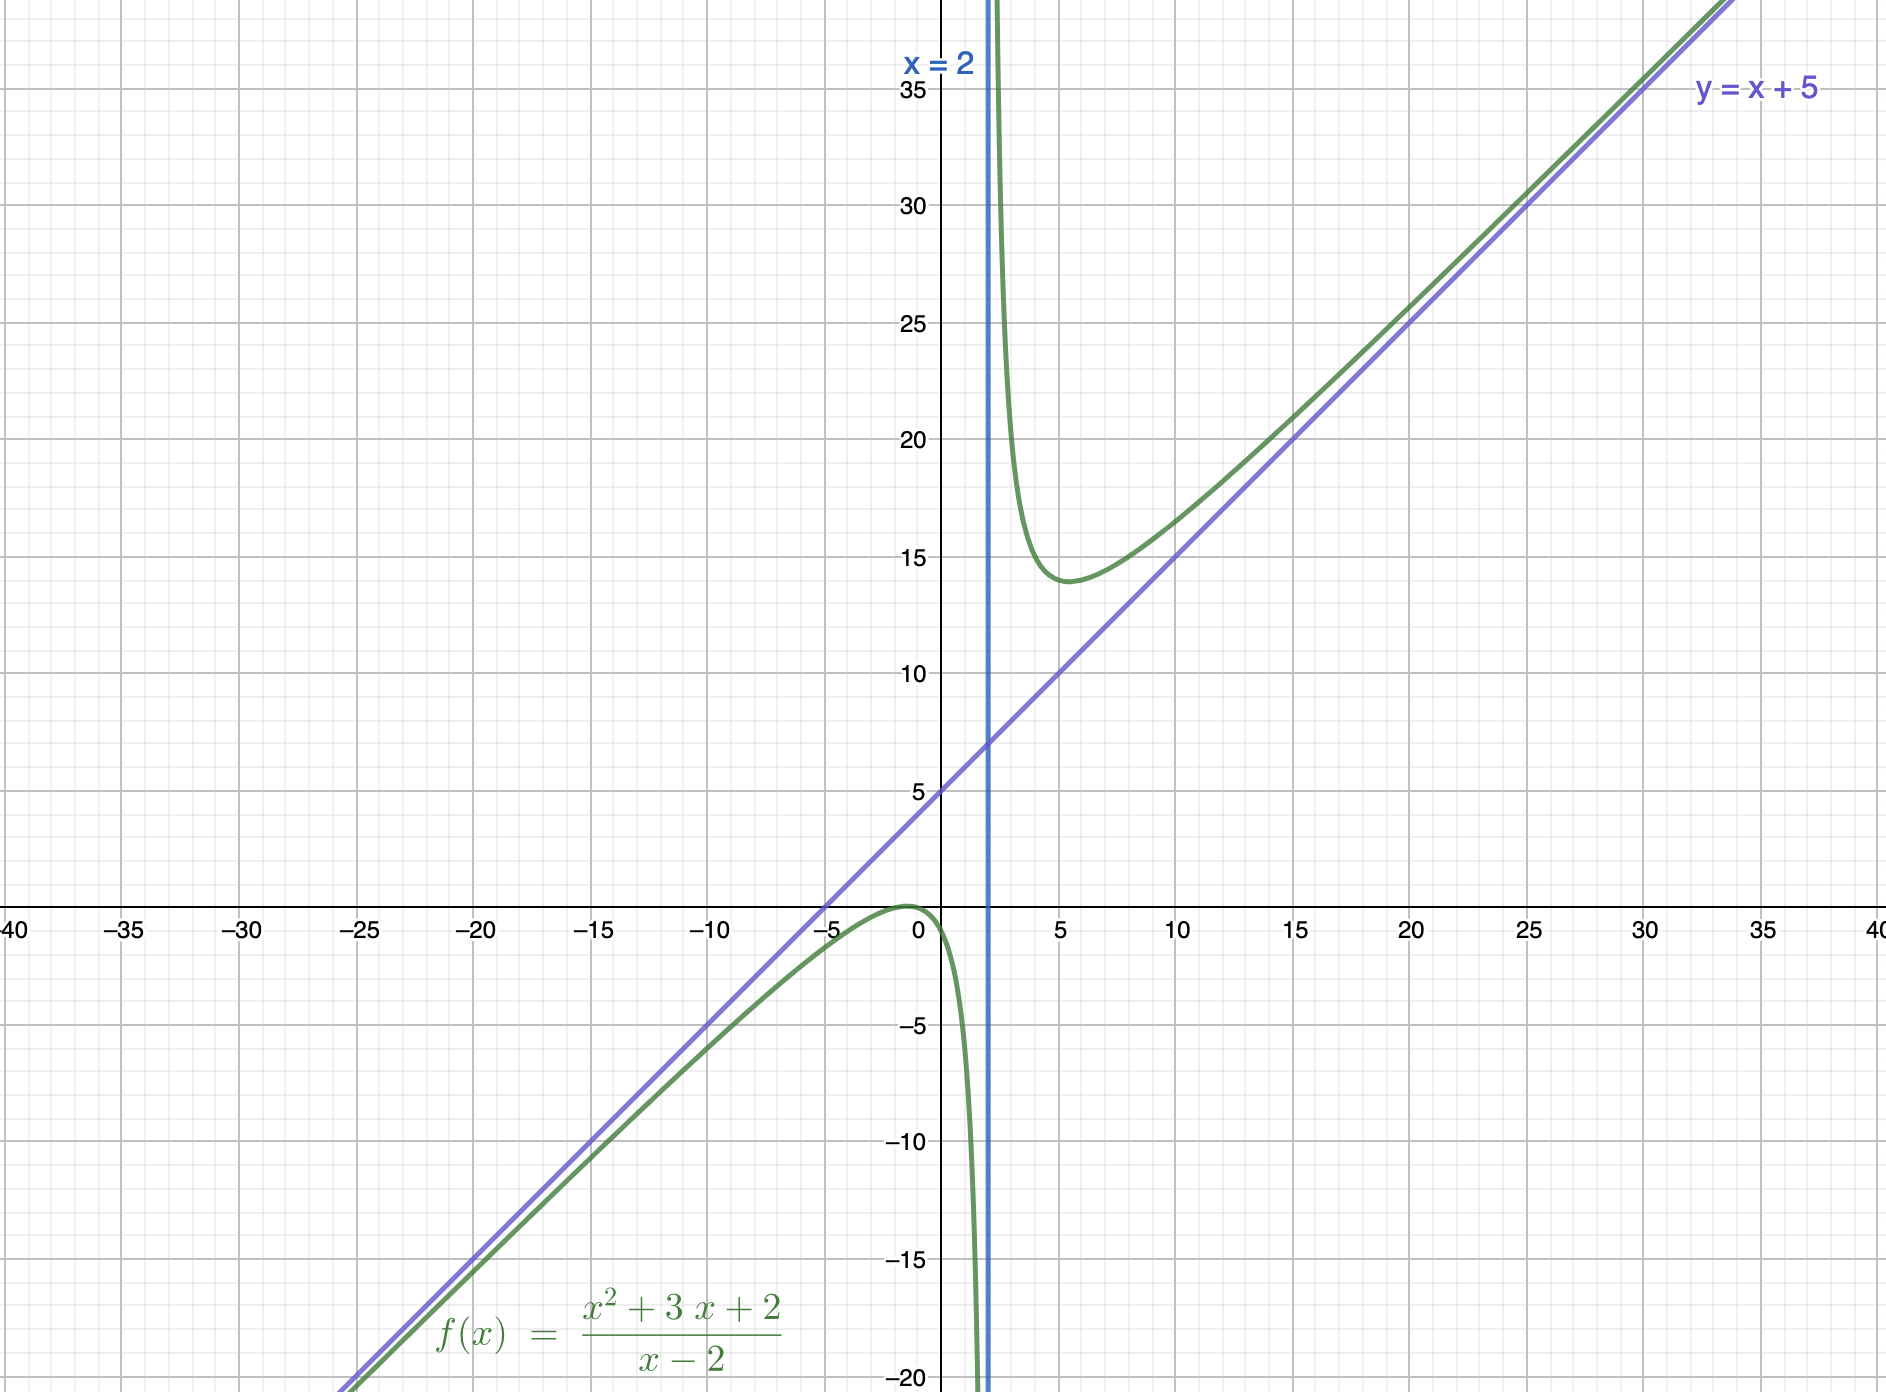
\includegraphics[width=0.8\textwidth]{Fig.2.8.jpg}
            \end{figure}
        \end{example}
        \begin{example}
            \textbf{Draw the diagram of $\displaystyle y=\frac{x^2-x-2}{x-1}$.}\\
            Intercept: $\displaystyle\left(0,2\right),\ \left(2,0\right),\ \left(-1,0\right)$\\
            V.A.: $x=1$\\
            O.A.: $y=x$ (Use long division)
            \begin{figure}[H]
                \centering
                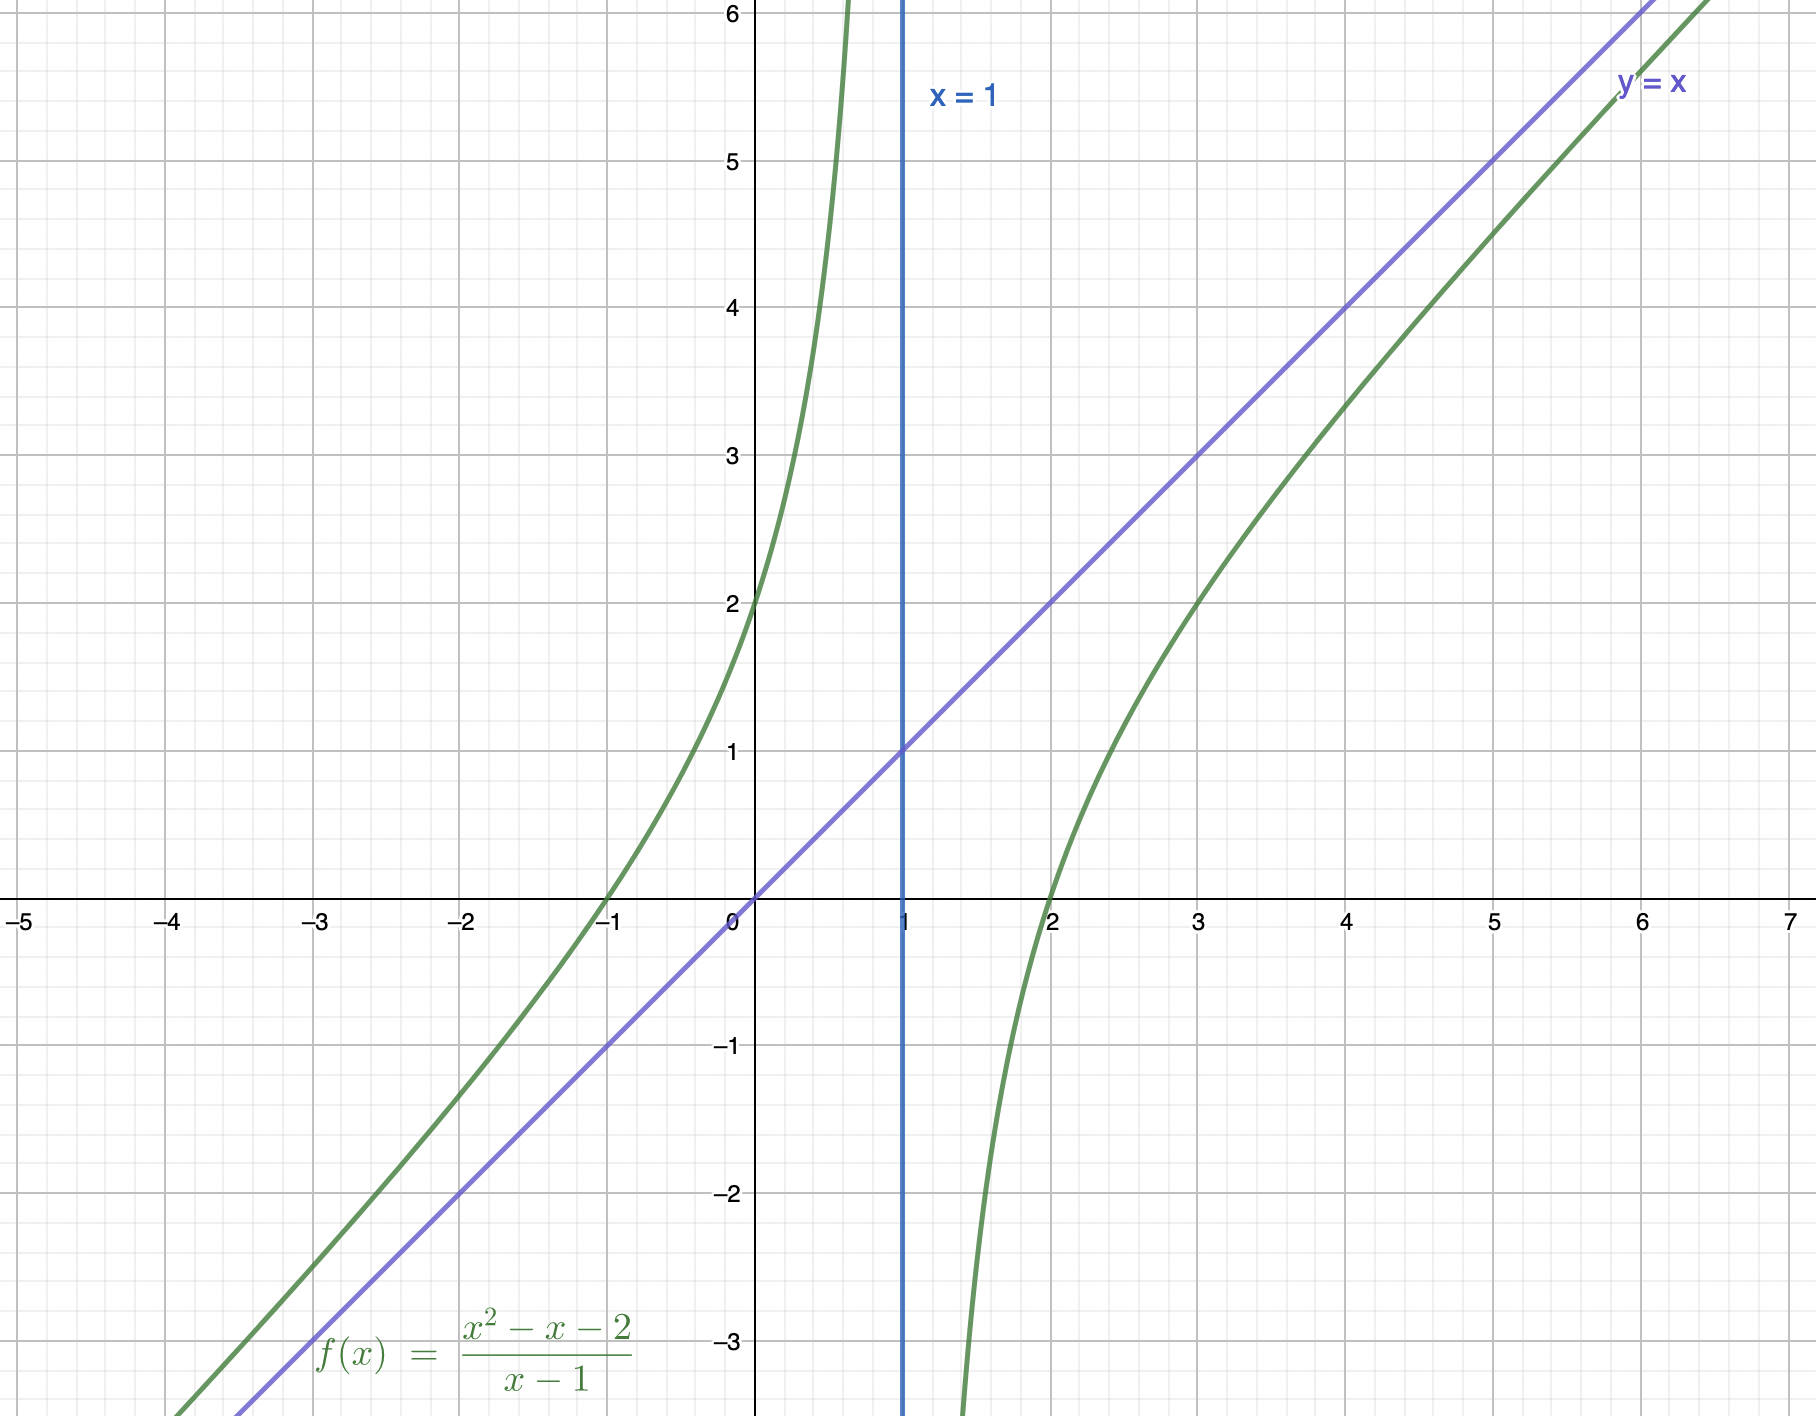
\includegraphics[width=0.8\textwidth]{Fig.2.9.jpg}
            \end{figure}
        \end{example}
    \end{itemize}
    \item When the function has asymptotes: 
    \begin{itemize}
        \item Denominator$=0$;
        \item $\log_a{0}$ (argument of a logarithm is 0)
    \end{itemize}
\end{enumerate}

\subsection{Transformation of Functions}
\begin{enumerate}
    \item \textbf{\color{red}{Translation}}: 
    \begin{itemize}
        \item $f(x+n)$ means translate $f(x)$ $n$ units to the left. 
        \item $f(x-n)$ means translate $f(x)$ $n$ units to the right. 
        \item $f(x)+n$ means translate $f(x)$ $n$ units upwards.
        \item $f(x)-n$ means translate $f(x)$ $n$ units downwards.
    \end{itemize}
    \item Use translation vector to represent translation: \\
    A vector ${\color{red}{\begin{pmatrix}a\\b\end{pmatrix}}}$ means $a$ units in the horizontal axis and $b$ units in the vertical axis. 
    \begin{example}
        A translation vector $\begin{pmatrix}-2\\3\end{pmatrix}$ means $f(x+2)+3$, 2 units to the left and 3 units upwards. 
    \end{example}
    \item \textbf{\color{red}{Reflections}}: 
    \begin{itemize}
        \item $f(-x)$ reflects in the {\color{red}{$y$-axis}}. 
        \item $-f(x)$ reflects in the {\color{red}{$x$-axis}}. 
        \item $f^{-1}(x)$ reflects in the {\color{red}{$y=x$}}.
        \item $-f(-x)$ reflects in the {\color{red}{origin}}.  
    \end{itemize}
    \item \textbf{\color{red}{Stretches}}: 
    \begin{itemize}
        \item $f(qx)$ is a horizontal stretch of a scale factor of $\displaystyle\frac{1}{q}$.
        \item $pf(x)$ is a vertical stretch of a scale factor of $p$.
    \end{itemize}
    \item When a graph is transforming, the points shift but the connection remains. 
    \item Sequence of transformation: 
    \begin{itemize}
        \item Do the horizontal translation before the horizontal stretch.
        \item The vertical translation is always after the vertical stretch.
        \item Vertical stretch $\rightarrow$ Reflection $\rightarrow$ Horizontal translation $\rightarrow$ Horizontal stretch $\rightarrow$ Vertical translation
    \end{itemize}
    \item \textbf{\color{red}{Modulus Function}}
    \begin{itemize}
        \item ${\color{red}{\left|f(x)\right|}}$: Fold everything below $x$-axis above $x$-axis. 
        \begin{example}
        \begin{figure}[H]
            \centering
            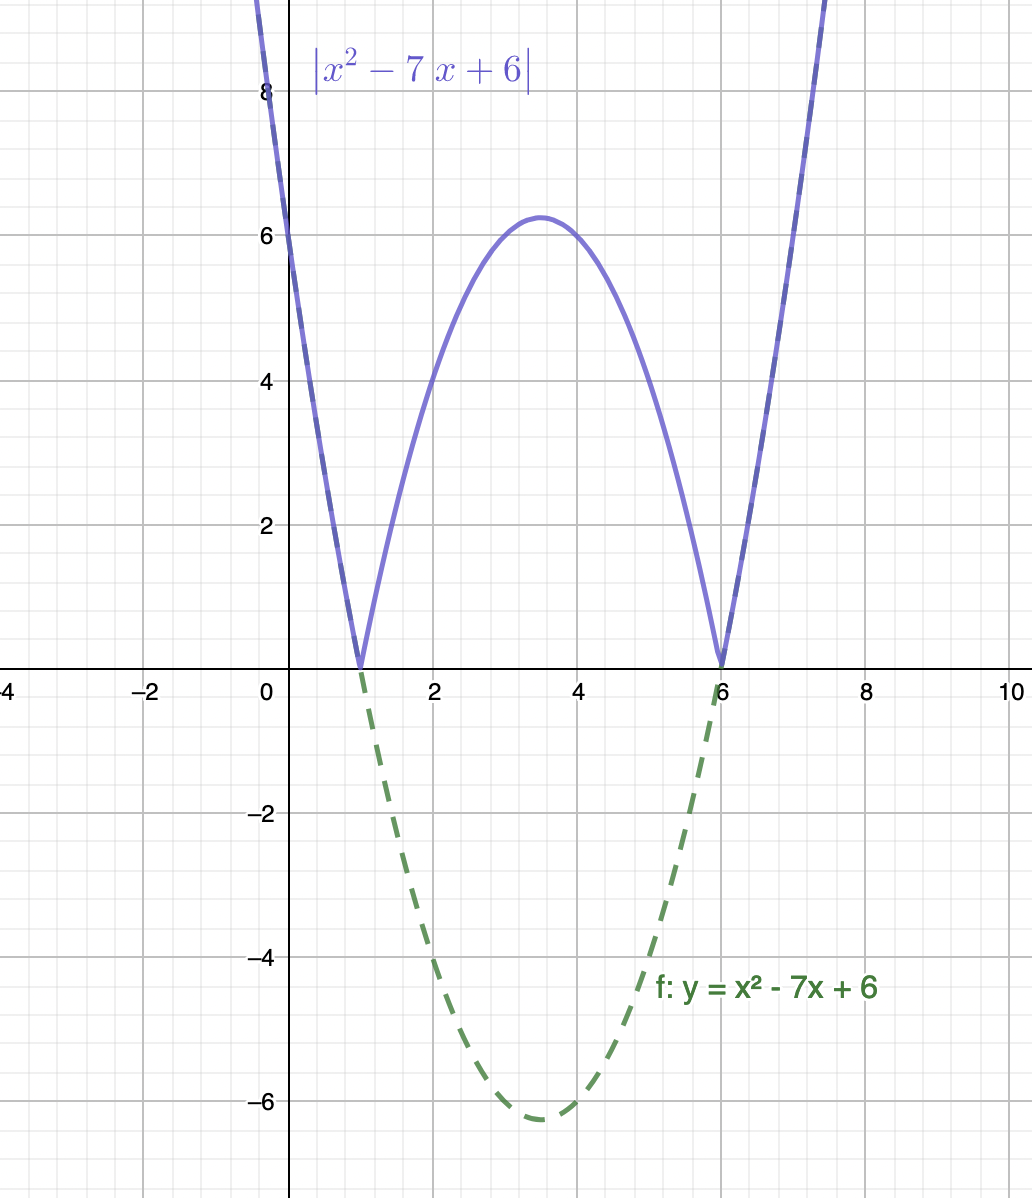
\includegraphics[width=0.48\textwidth]{Fig.2.10.jpg}
        \end{figure}
        \end{example}
        \item ${\color{red}{f(\left|x\right|)}}$: Reflect everthing on the right of $y$-axis to the left. 
        {\color{green}{Since $|x|$ must be positive, $|x|=|-x|\ \Rightarrow\ f(-x)=f(x)$, which is an even function.}}
        \begin{example}
            \begin{figure}[H]
                \centering
                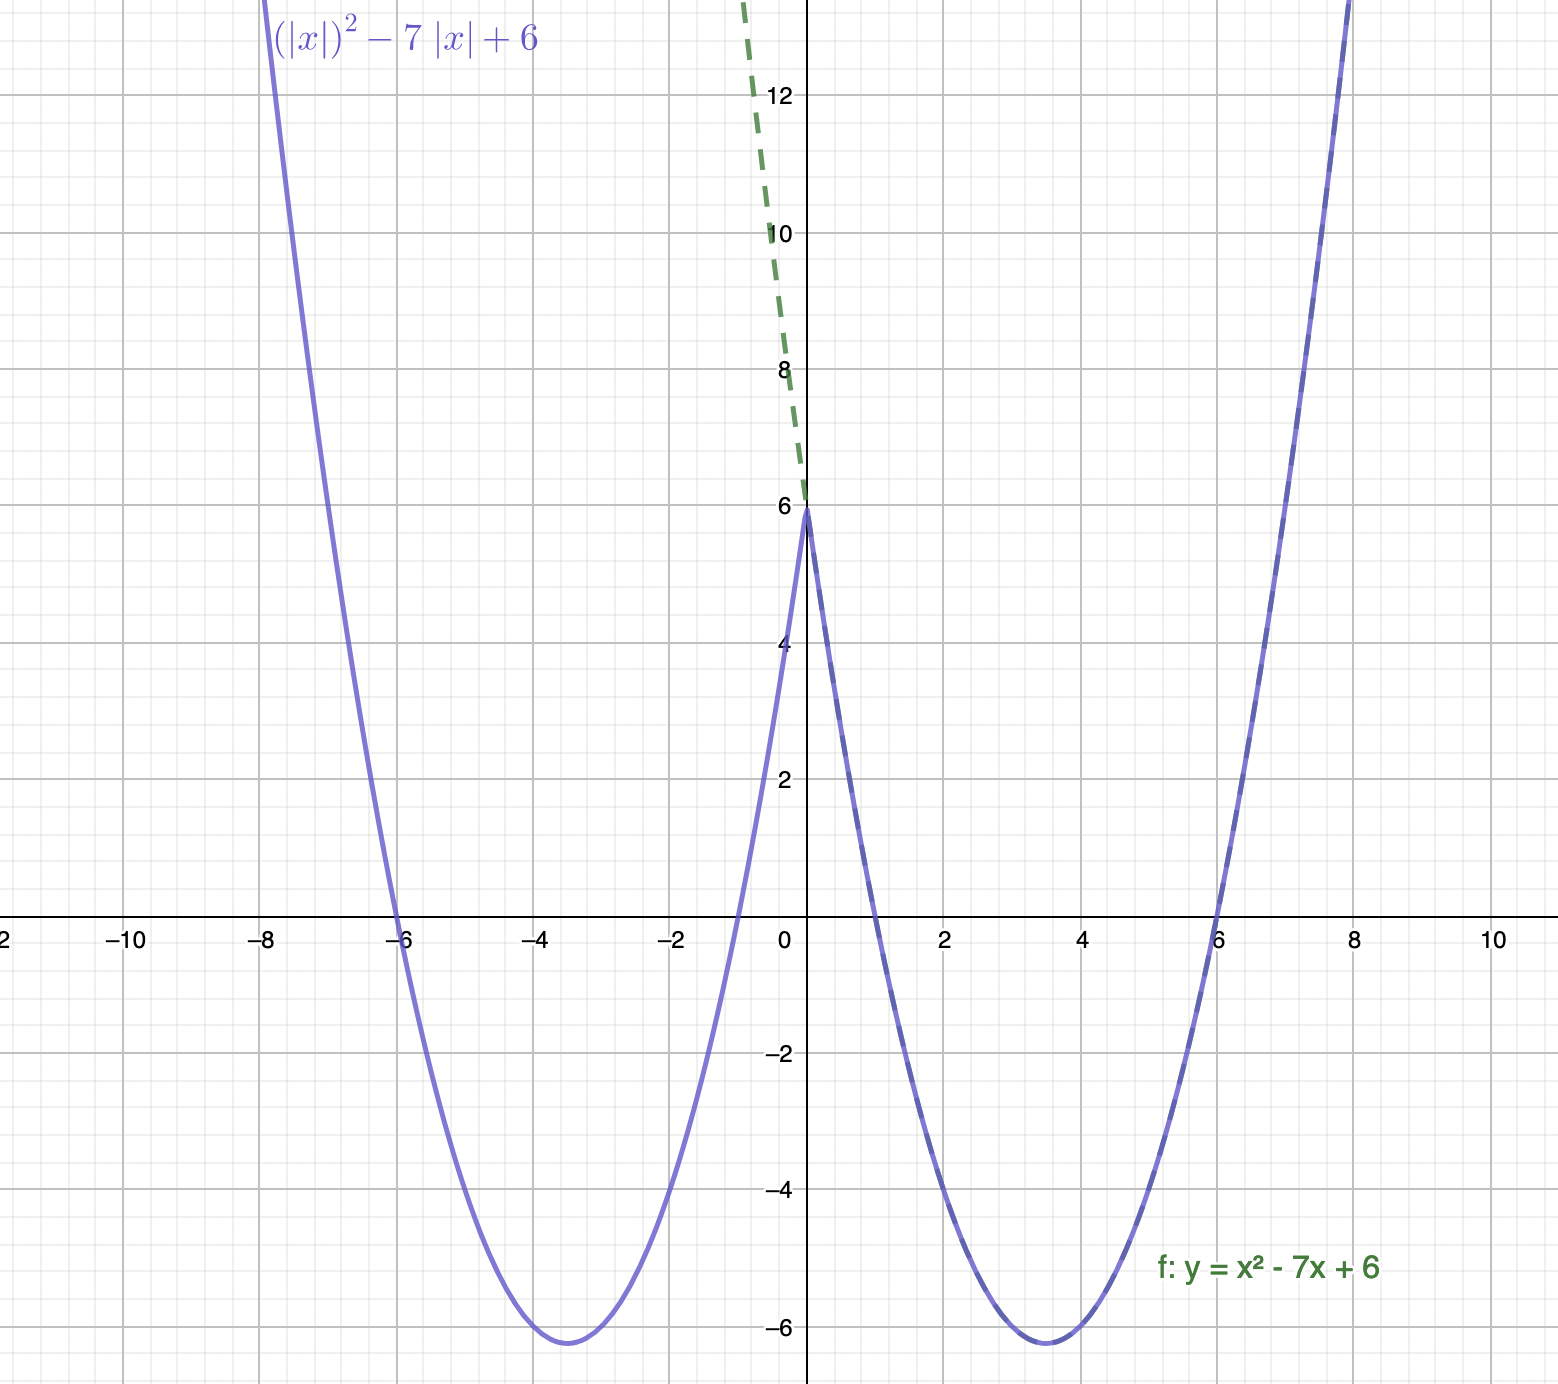
\includegraphics[width=0.6\textwidth]{Fig.2.11.jpg}
            \end{figure}
            \end{example}
    \end{itemize}
    \item \textbf{\color{red}{Reciprocal of $f(x)$}}
    \begin{itemize}
        \item Table of Summary: 
        \begin{center}
        \begin{tabular}{c|c}
            $f(x)$&$g(x)=\frac{1}{x}$\\\hline
            $f(a)=0$&Line $x=a$ is vertical asymptote\\\hline
            Line $x=a$ is vertical asymptote&$g(a)=0$\\\hline
            $f(x)\to\infty$&$g(x)\to 0$\\\hline
            $f(x)\to 0$&$g(x)\to\infty$\\\hline
            Line $y=b$ is horizontal asymptote&Line $y=\frac{1}{b}$ is horizontal asymptote\\\hline
            $f(x)=a$&$g(x)=\frac{1}{a}$
        \end{tabular}
        \end{center}
        \item When $f(x)$ increases, $g(x)$ decreases. 
    \end{itemize}
\end{enumerate}

\subsection{Exponential and Logarithmic Functions}
\begin{enumerate}
    \item Exponential functions: 
    \begin{itemize}
        \item $f(x)=a^x,\ a>1$ (increasing) and $0<a<1$ (decreasing). 
        \item $f(x)=a^x$ and $g(x)=\displaystyle\left(\frac{1}{a}\right)^x$ are symmetric to the $y$-axis. 
        \begin{proof}
            $$g(x)=\left(\frac{1}{a}\right)^x=(a^-1)^x=a^{-x}=f(-x).$$
        \end{proof}
        \item Domain: $x\in\R$, Range: $y>0$
        \item Common point: $(0, 1)$; common H.A.: $y=0$
        \item Graph: 
        \begin{figure}[H]
            \centering
            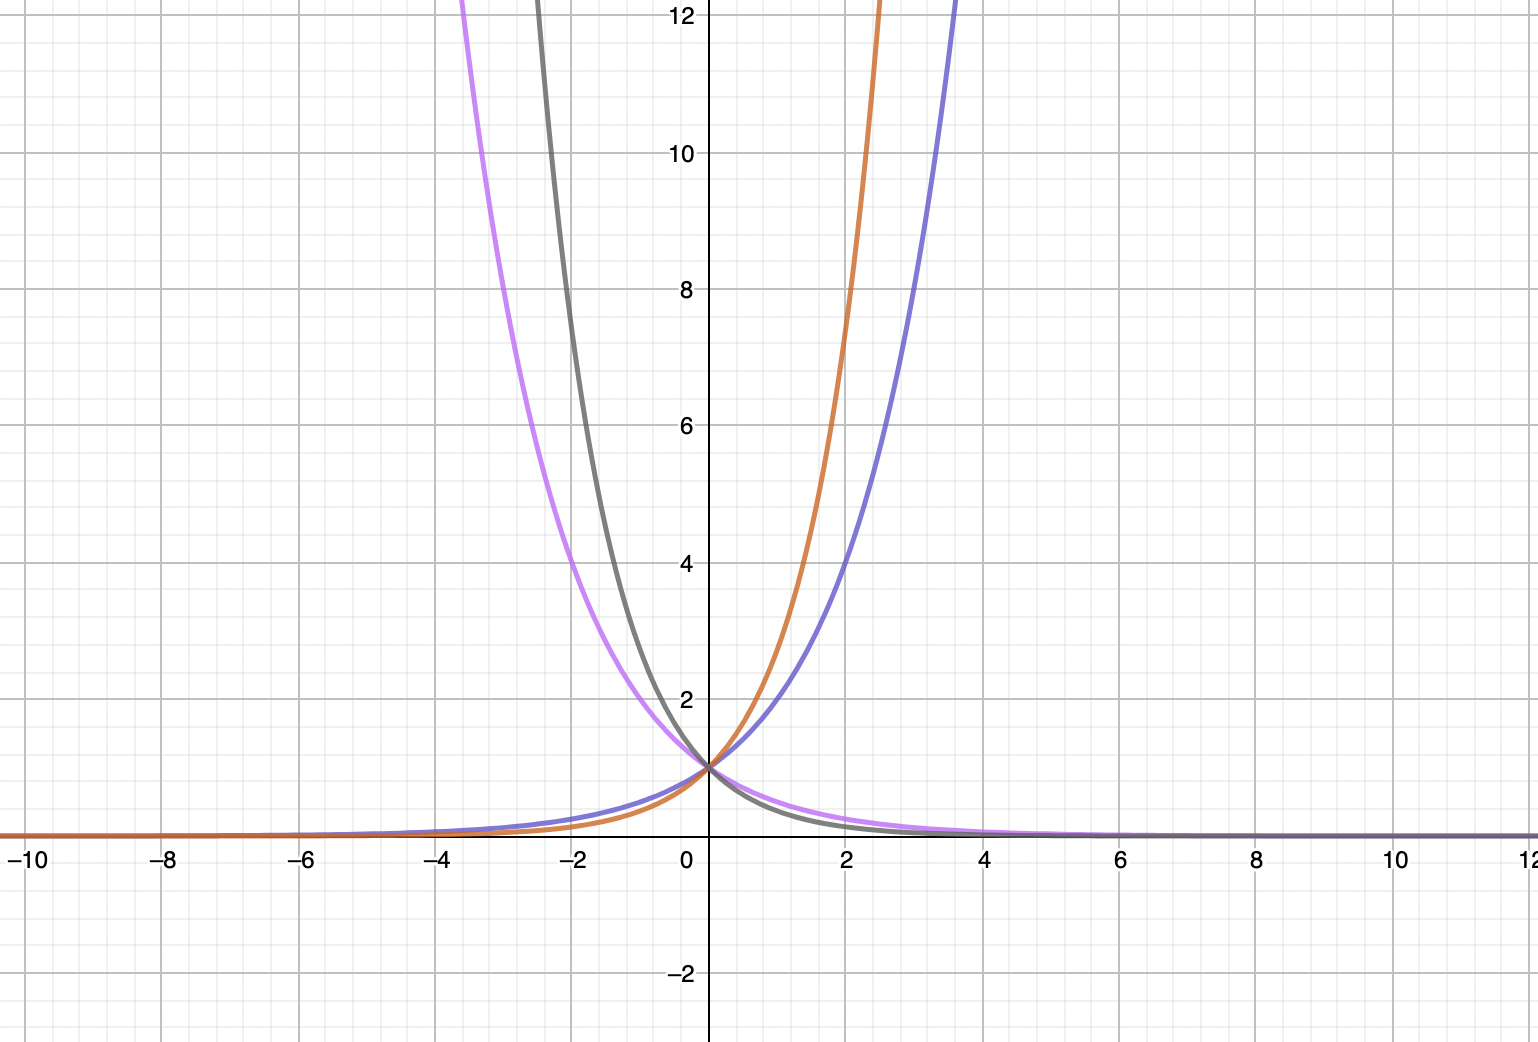
\includegraphics[width=0.48\textwidth]{Fig.2.12.jpg}
        \end{figure}
    \end{itemize}
    \item Logarithmic functions: 
    \begin{itemize}
        \item $f(x)=\log_a{x}=g^{-1}(x), g(x)=a^x$.
        \item Common point: $(1,0)$; common V.A.: $x=0$.
        \item $f(x)=\log_a{x}$ and $g(x)=\log_{\frac{1}{a}}{x}$ are symmetric to the $x$-axis.
        \begin{proof}
            $$\log_{\frac{1}{a}}{x}=\frac{\log_a{x}}{\log_\frac{1}{a}a}=\frac{\log_ax}{-1}=-\log_ax,$$
            $$\therefore g(x)=\log_\frac{1}{a}x=-\log_ax=-f(x).$$
        \end{proof}
        \item When $a>1$, increasing function; when $0<a<1$, decreasing function. 
        \item Domain: $x>0$, Range: $y\in\R$
        \item Graph: 
        \begin{figure}[H]
            \centering
            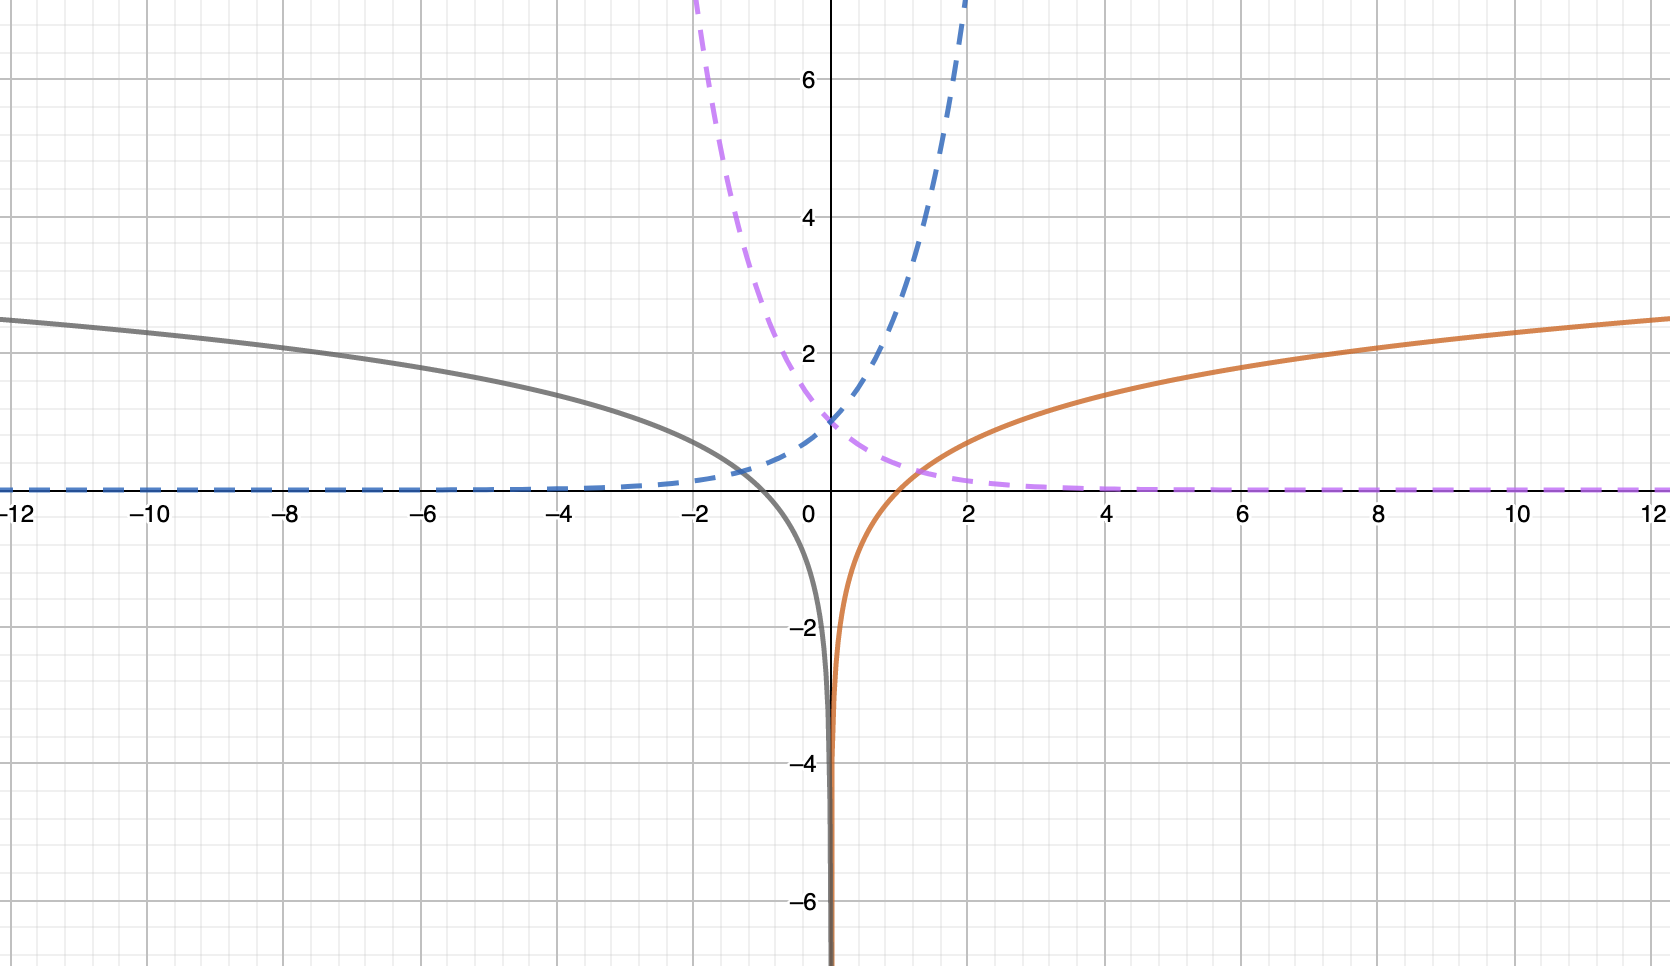
\includegraphics[width=0.7\textwidth]{Fig.2.13.jpg}
        \end{figure}
    \end{itemize}
    \item Solving logarithmic equations.
    \item Solving exponential equations: take logarithm on both sides.
\end{enumerate}

\newpage
\section{Topic 3 Trigonometry and Geometry}
\subsection{Trigonometry}
\subsubsection{Radian}
\begin{enumerate}
  \item Radian as the unit of angle: 
  \begin{itemize}
    \item $${\color{red}{\pi\ \text{rad}=180^\circ}}$$
    \item rad can be omitted. {\color{green}{i.e., $\widehat{A}=1$ means angle $A$ is $1$ radian.}}
    \item Unit coversion: $${\color{red}{\text{degree}\times\frac{\pi}{180^\circ}=\text{radian;\ radian}\times\frac{180^\circ}{\pi}=\text{degree}.}}$$
  \end{itemize}
  \item Arc: 
  \begin{itemize}
    \item The \textbf{\color{red}{circumference}} (perimeter) is $2\pi r$.
    \begin{figure}[H]
      \centering
      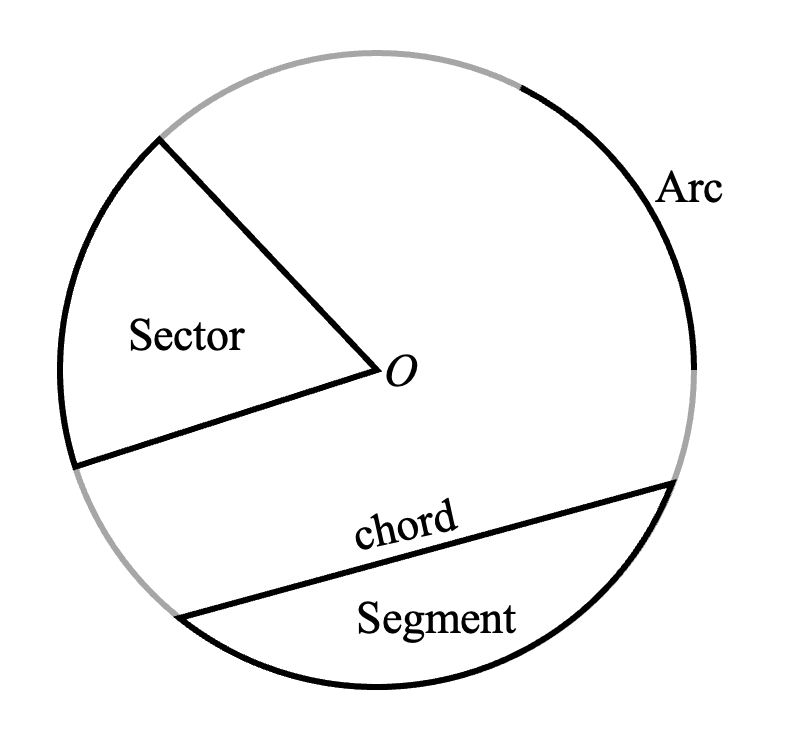
\includegraphics[width=0.5\textwidth]{Fig.3.18.jpg}
    \end{figure}
    \item If the angle of the arc is $\theta$ (in radian), the length of $\text{arc}(l)=r\cdot\theta$.
    \item The area of a sector: $$\color{red}A=\frac{1}{2}r^2\theta.$$
    \item The area of a segment: $$\color{red}A=\frac{1}{2}r^2(\theta-\sin\theta).$$(Proof: the area of the triangle according to the sine rule is $\frac{1}{2}ab\sin C$)
  \end{itemize}
\end{enumerate}

\subsubsection{Solution of Triangle}
\begin{enumerate}
  \item Define sine, cosine, and tangent: 
  \begin{definition}
    \begin{figure}[H]
      \centering
      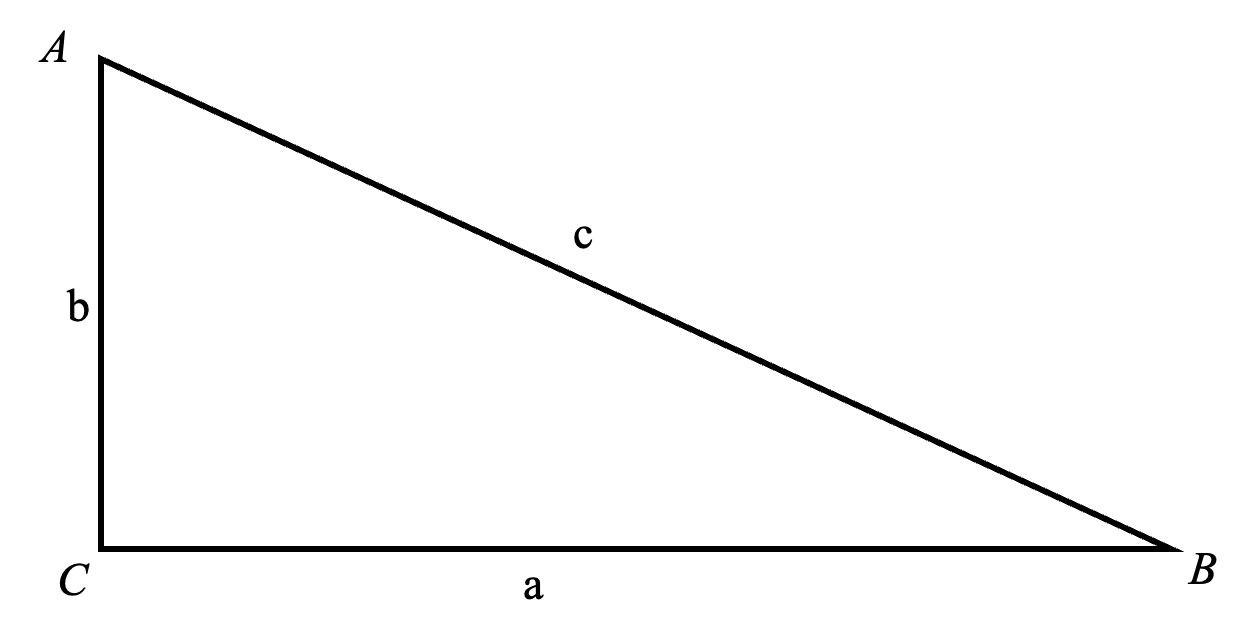
\includegraphics[width=0.5\textwidth]{Fig.3.19.jpg}
    \end{figure}
    $$\sin A=\frac{a}{c},\ \sin B=\frac{b}{c};$$
    $$\cos A=\frac{b}{c},\ \cos B=\frac{a}{c};$$
    $$\tan A=\frac{a}{b},\ \tan B=\frac{b}{a}.$$
  \end{definition}
  \item The Sine Rule: 
  \begin{theorem}
    $${\color{red}{\frac{\sin A}{a}=\frac{\sin B}{b}=\frac{\sin C}{c}}}.$$
  \end{theorem}
  \begin{itemize}
    \item The bigger the angle, the longer the side. 
    \item Area of a triangle: $${\color{red}{A=\frac{1}{2}ab\sin C}}.$$
  \end{itemize}
  \item The Consine Rule: 
  \begin{theorem}
    $${\color{red}{b^2+c^2-a^2=2bc\cdot\cos A}};$$
    $${\color{red}{a^2+c^2-b^2=2ac\cdot\cos B}};$$
    $${\color{red}{a^2+b^2-c^2=2ab\cdot\cos C}}.$$
  \end{theorem}
  \item Inverse Trigonometric Functions: 
  \begin{definition}
    $$\sin^{-1}\theta=\arcsin\theta;$$
    $$\cos^{-1}\theta=\arccos\theta;$$
    $$\tan^{-1}\theta=\arctan\theta.$$
  \end{definition}
  \item Ambiguity of Sine Rule: 
  $${\color{red}{\sin\theta=\sin(180^\circ-\theta)\text{ OR }\sin\theta=\sin(\pi-\theta)}}.$$
  \item Angle of Elevation and Depression: 
  \begin{definition}
    \begin{figure}[H]
      \centering
      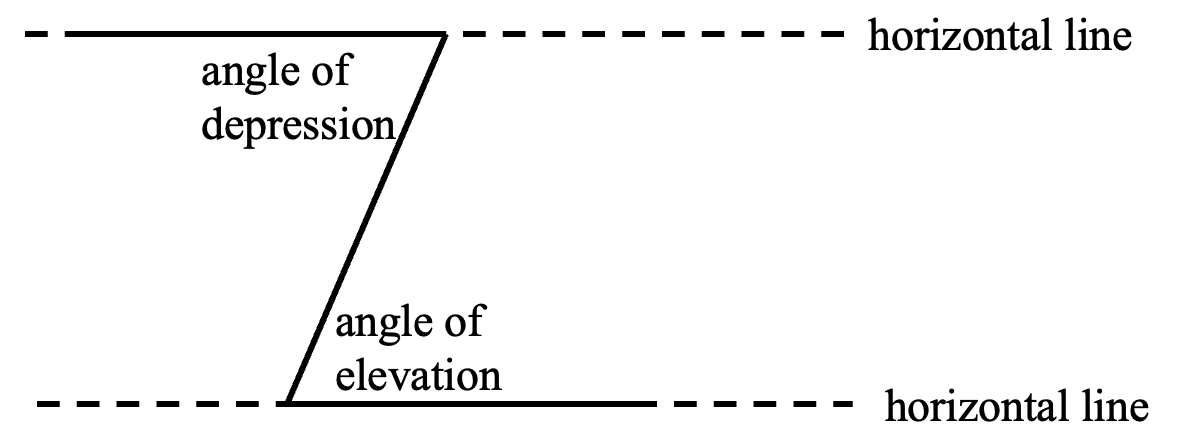
\includegraphics[width=0.8\textwidth]{Fig.3.20.jpg}
    \end{figure}
    \begin{itemize}
    \item \textbf{\color{red}{Angle of Elevation}} is the angle "up" from horizontal. 
    \item \textbf{\color{red}{Angle of Depression}} is the angle "down" from horizontal. 
    \end{itemize}
  \end{definition}
  \item Bearing: 
  \begin{itemize}
    \item Bearing is a way of describing direction. 
    \item All bearings are measured {\color{red}{clockwise}} from the {\color{red}{North}} direction. 
    \begin{figure}[H]
      \centering
      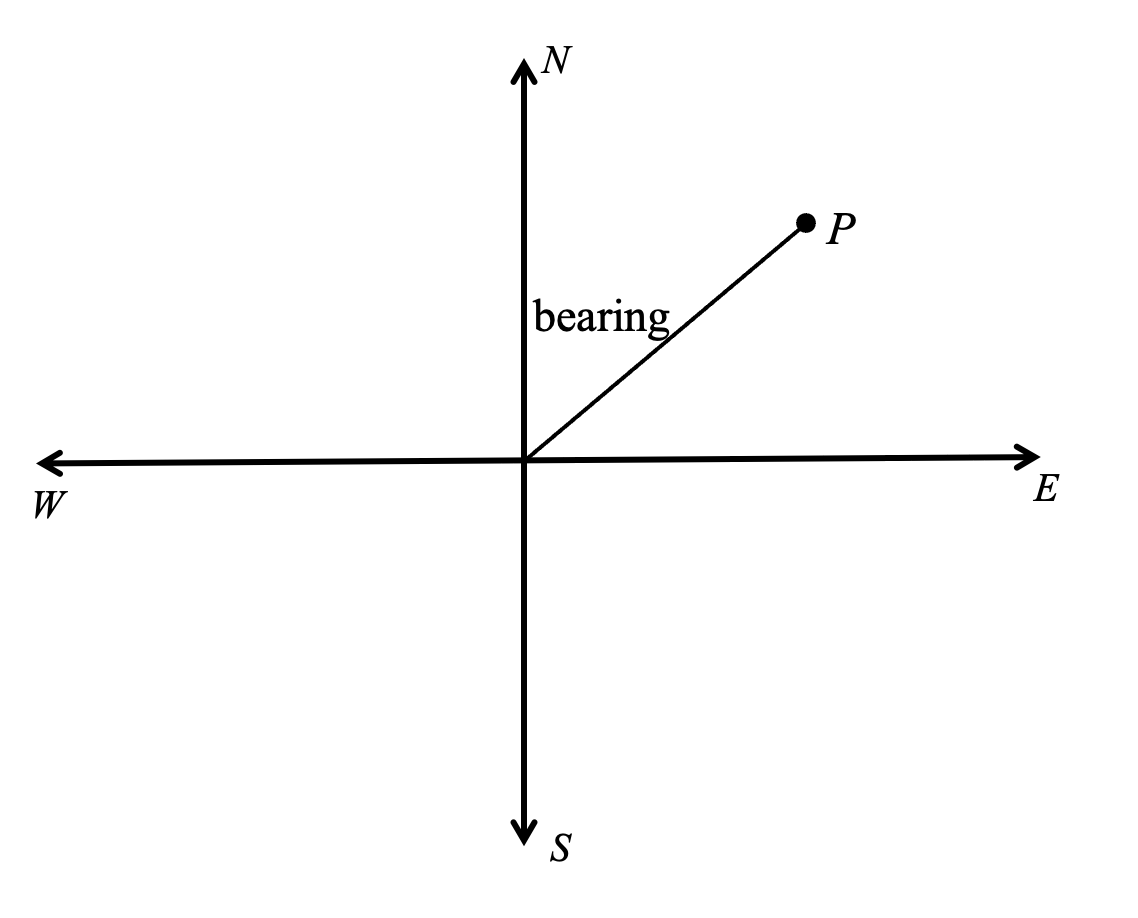
\includegraphics[width=0.5\textwidth]{Fig.3.21.jpg}
    \end{figure}
  \item Bearing of $A$ from $B$: construct at $B$.\\
  {\color{green}{N.B.: Bearing of $A$ from $B$ is different from bearing of $B$ from $A$.}}
  \end{itemize}
\end{enumerate}

\subsubsection{Definition of Trigonometric Function}
\begin{enumerate}
  \item Unit Circle: 
  \begin{itemize}
    \item Center at $(0,0)$ with a radius of $1$.
    \begin{figure}[H]
      \centering
      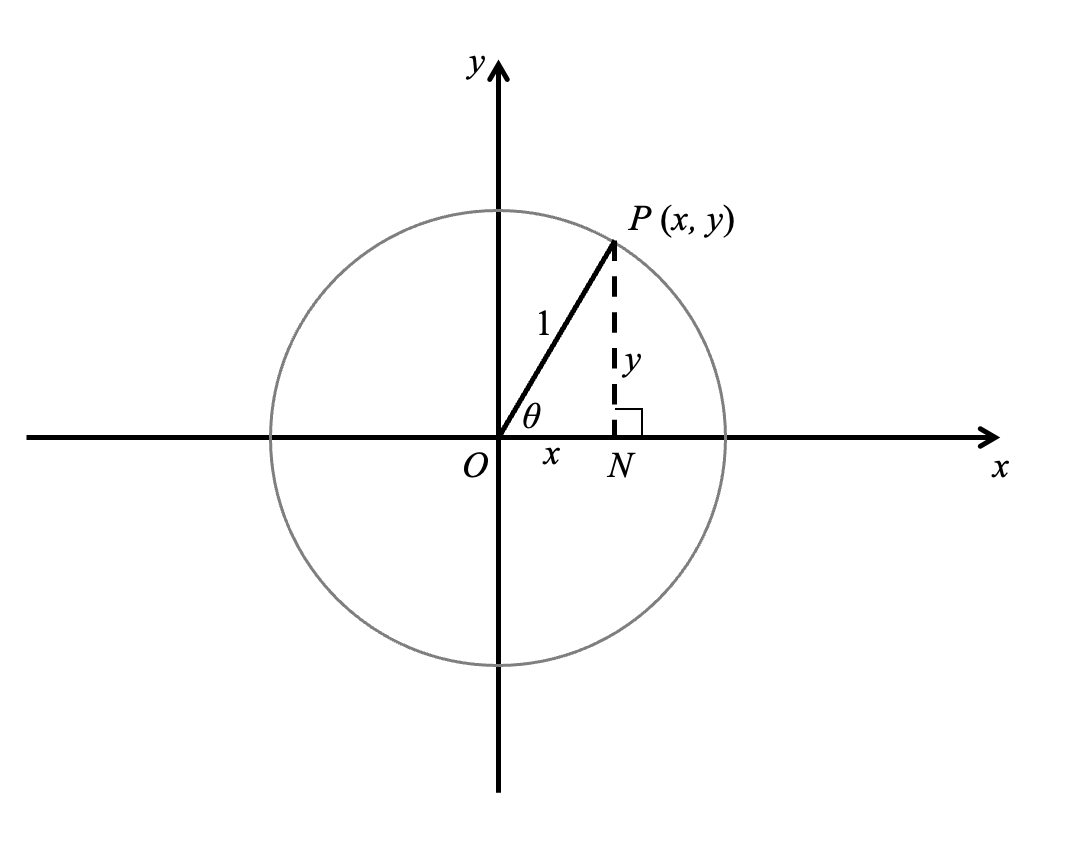
\includegraphics[width=0.5\textwidth]{Fig.3.22.jpg}
    \end{figure}
    \item If an angel $\theta$ opens in a counterclockwise direction, then $\theta$ is positive. \\
    If an angle $\theta$ opens in a clockwise direction, then $\theta$ is negative. 
    \item In the diagram, $\theta=\theta+2k\pi,\ k\in\Z.$
    \item $$\sin\theta=\frac{PN}{OP}=\frac{y}{1}=y; $$
    $$\cos\theta=\frac{ON}{OP}=\frac{x}{1}=x; $$
    $$\tan\theta=\frac{PN}{ON}=\frac{y}{x}=\frac{\sin\theta}{\cos\theta}; $$
    \item In $Q_1$ and $Q_2$, $\sin\theta$ will be positive.\\
    In $Q_1$ and $Q_4$, $\cos\theta$ will be positive.\\
    In $Q_1$ and $Q_3$, $\tan\theta$ will be positive.\\
    $\Rightarrow$ CAST: 
    \begin{figure}[H]
      \centering
      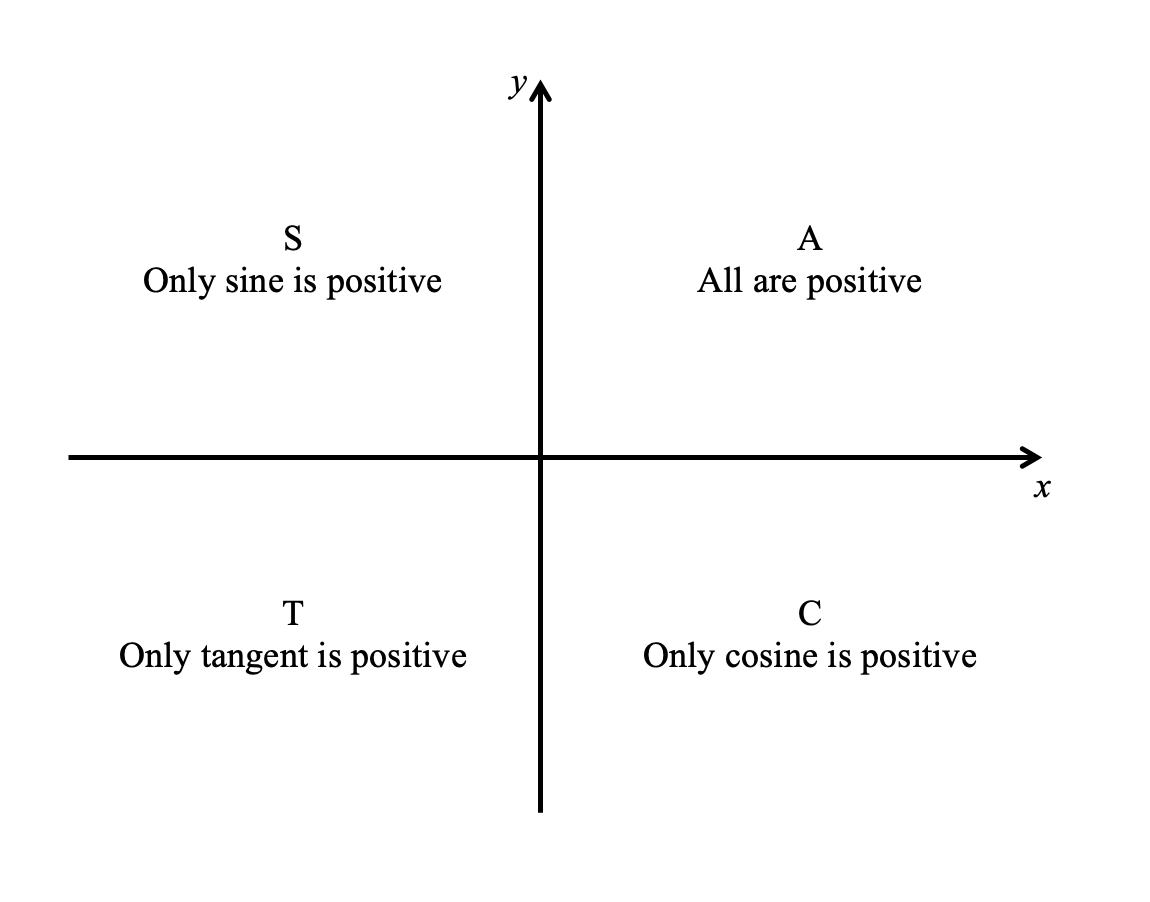
\includegraphics[width=0.5\textwidth]{Fig.3.23.jpg}
    \end{figure}
  \end{itemize}
  \item Special Angles: 
  \begin{multicols}{2}
    $$\sin0^\circ=0=\cos90^\circ$$
    $$\sin30^\circ=\frac{1}{2}=\cos60^\circ$$
    $$\sin45^\circ=\frac{\sqrt{2}}{2}=\cos45^\circ$$
    $$\sin60^\circ=\frac{\sqrt{3}}{2}=\cos30^\circ$$
    $$\sin90^\circ=1=\cos0^\circ$$
    $$\tan0^\circ=\frac{\sin0^\circ}{\cos0^\circ}=0$$
    $$\tan30^\circ=\frac{\sin30^\circ}{\cos30^\circ}=\frac{\sqrt{3}}{3}$$
    $$\tan45^\circ=\frac{\sin45^\circ}{\cos45^\circ}=1$$
    $$\tan60^\circ=\frac{\sin60^\circ}{\cos60^\circ}=\sqrt{3}$$
    $$\tan90^\circ=\frac{\sin90^\circ}{\cos90^\circ}=\infty$$
  \end{multicols}
  \item Relative Acute Angles (RAA): 
  \begin{itemize}
    \item Acute angle is the angle with $x$-axis.
    \item The absolute value of angles have the same acute angle is the same. 
    \begin{example}
      \begin{enumerate}
        \item $30^\circ,\ 150^\circ,\ 210^\circ,\ 330^\circ$ have the same acute angle. \\
        $\therefore \left|\sin30^\circ\right|=\left|\sin150^\circ\right|=\left|\sin210^\circ\right|=\left|\sin330^\circ\right|.$
        \item $$\tan220^\circ=\tan40^\circ;\ \cos215^\circ=-\cos35^\circ$$
        \begin{figure}[H]
          \centering
          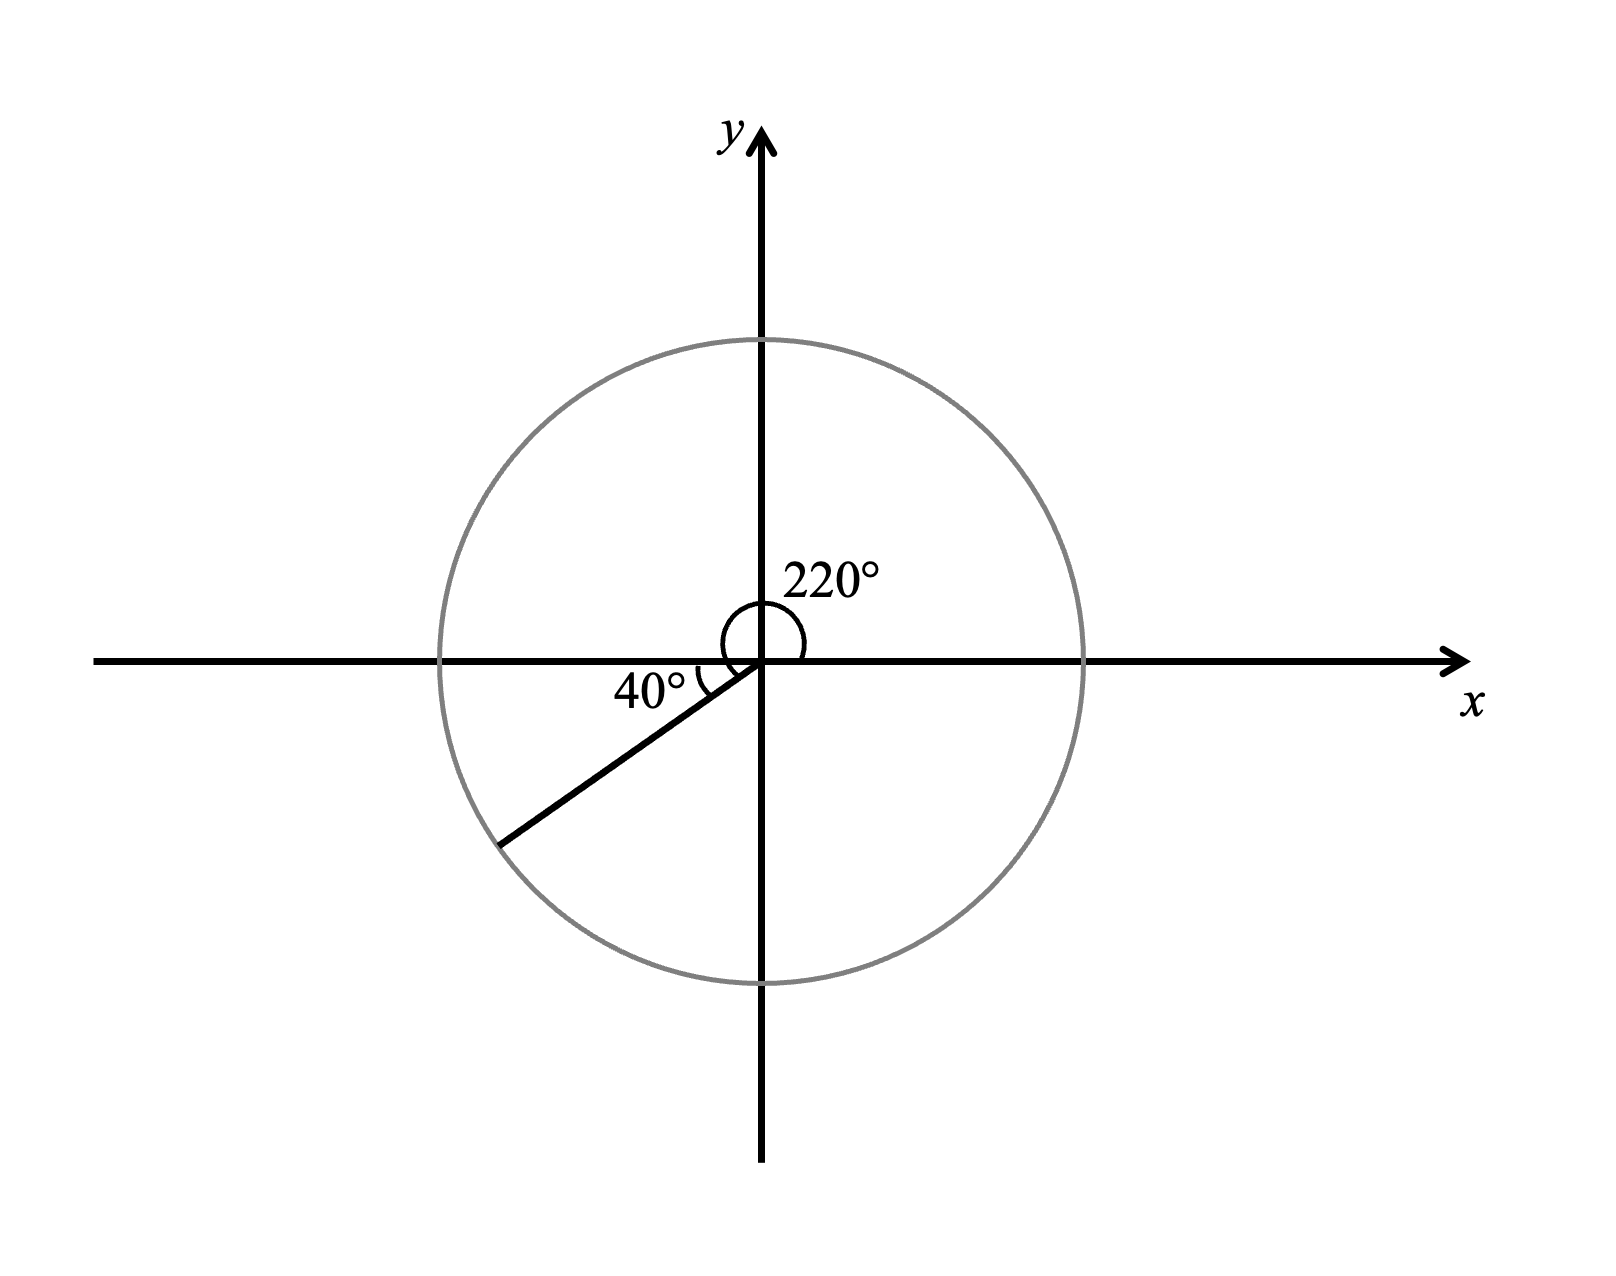
\includegraphics[width=0.5\textwidth]{Fig.3.24.jpg}
        \end{figure}
      \end{enumerate}
    \end{example}
  \end{itemize}
\end{enumerate}

\subsubsection{Trigonometric Identity}
\begin{enumerate}
  \item Pythagorean's Identity: 
  $${\color{red}{\sin^2\theta+\cos^2\theta\equiv1}}.$$
  \begin{proof}
    $$\begin{aligned}
      a^2+b^2=c^2&\Rightarrow\frac{a^2}{c^2}+\frac{b^2}{c^2}=1\\
      &\Rightarrow\sin^2\theta+\cos^2\theta=1.
    \end{aligned}$$
  \end{proof}
  \item Definition of Tangent: 
  \begin{itemize}
    \item $${\color{red}{\tan\theta=\frac{\sin\theta}{\cos\theta}}};$$
    \item $${\color{red}{\cot\theta=\frac{1}{\tan\theta}}};$$
    \item $${\color{red}{\sec\theta=\frac{1}{\cos\theta}}};$$
    \item $${\color{red}{\csc\theta=\frac{1}{\sin\theta}}}.$$
  \end{itemize}
  \item Extended Pythagorean's Identity: 
  $${\color{red}{\tan^2\theta+1=\sec^2\theta}};$$
  $${\color{red}{\cot^2\theta+1=\csc^2\theta}}.$$
  \begin{proof}
    $$\begin{aligned}
      \sin^2\theta+\cos^2\theta=1\Rightarrow&\frac{\sin^2\theta}{\cos^2\theta}+\frac{\cos^2\theta}{\cos^2\theta}=\frac{1}{\cos^2\theta}\Rightarrow\tan^2+1=\sec^2\theta;\\
      &\frac{\sin^2\theta}{\sin^2\theta}+\frac{\cos^2\theta}{\sin^2\theta}=\frac{1}{\sin^2\theta}\Rightarrow\cot^2\theta+1=csc^2\theta.
    \end{aligned}$$
    {\color{green}{N.B.: a reflex angle is an angle bigger than $180^\circ$, smaller than $360^\circ$.}}
  \end{proof}
  \item Compound Angle Formula: 
  $${\color{red}{\cos(A+B)=\cos{A}\cos{B}-\sin{A}\sin{B}}};$$
  $${\color{red}{\cos(A-B)=\cos{A}\cos{B}+\sin{A}\sin{B}}};$$
  $${\color{red}{\sin(A+B)=\sin{A}\cos{B}+\cos{A}\sin{B}}};$$
  $${\color{red}{\sin(A-B)=\sin{A}\cos{B}-\cos{A}\sin{B}}};$$
  \begin{example}
    \textbf{Find the exact value of $\cos{\frac{\pi}{12}}$.}
    $$\begin{aligned}
      \cos{\frac{\pi}{12}}&=\cos{\frac{\pi}{4}-\frac{\pi}{6}}\\
      &=\cos{\frac{\pi}{4}}\cos\frac{\pi}{6}+\sin\frac{\pi}{4}\sin\frac{\pi}{6}\\
      &=\frac{\sqrt{2}}{2}\times\frac{\sqrt{3}}{2}+\frac{\sqrt{2}}{2}\times\frac{1}{2}=\frac{\sqrt{6}+\sqrt{2}}{4}.
    \end{aligned}$$
  \end{example}
  $${\color{red}{\tan{(A+B)=\frac{\tan{A}+\tan{B}}{1-\tan{A}\tan{B}}}}}.$$
  \begin{proof}
    $$\begin{aligned}
      \tan{(A+B)}=\frac{\sin{(A+B)}}{\cos{(A+B)}}&=\frac{\sin{A}\cos{B}+\cos{A}\sin{B}}{\cos{A}\cos{B}-\sin{A}\sin{B}}\\
      &=\frac{\frac{\sin{A}\cos{B}}{\cos{A}\cos{B}}+\frac{\cos{A}\sin{B}}{\cos{A}\cos{B}}}{\frac{\cos{A}\cos{B}}{\cos{A}\cos{B}}-\frac{\sin{A}\sin{B}}{\cos{A}\cos{B}}}\\
      &=\frac{\tan{A}+\tan{B}}{1-\tan{A}\tan{B}}.
    \end{aligned}$$
  \end{proof}
  $${\color{red}{\tan{(A-B)}=\frac{\tan{A}-\tan{B}}{1+\tan{A}\tan{B}}}}.$$
  \item In the linear function $y=mx+b$, ${\color{red}{m=\tan\theta}}$, where $\theta$ is the angle between the line and the positive $x$-axis. 
  \item Double Angle Formula: 
  $${\color{red}{\cos{(2\theta)}=\cos^2\theta-\sin^2\theta=2\cos^2\theta-1=1-2\sin^2\theta}};$$
  $${\color{red}{\sin{(2\theta)}=2\sin\theta\cos\theta}};$$
  $${\color{red}{\tan{(2\theta)}=\frac{2\tan\theta}{1-\tan^2\theta}}}.$$
  \item Proving Identities. 
\end{enumerate}

\subsubsection{Trigonometric Functions and Transformation}
\begin{enumerate}
  \item Sine: Odd function: $\sin{(-x)}=-\sin{x}$.
  \begin{figure}[H]
    \centering
    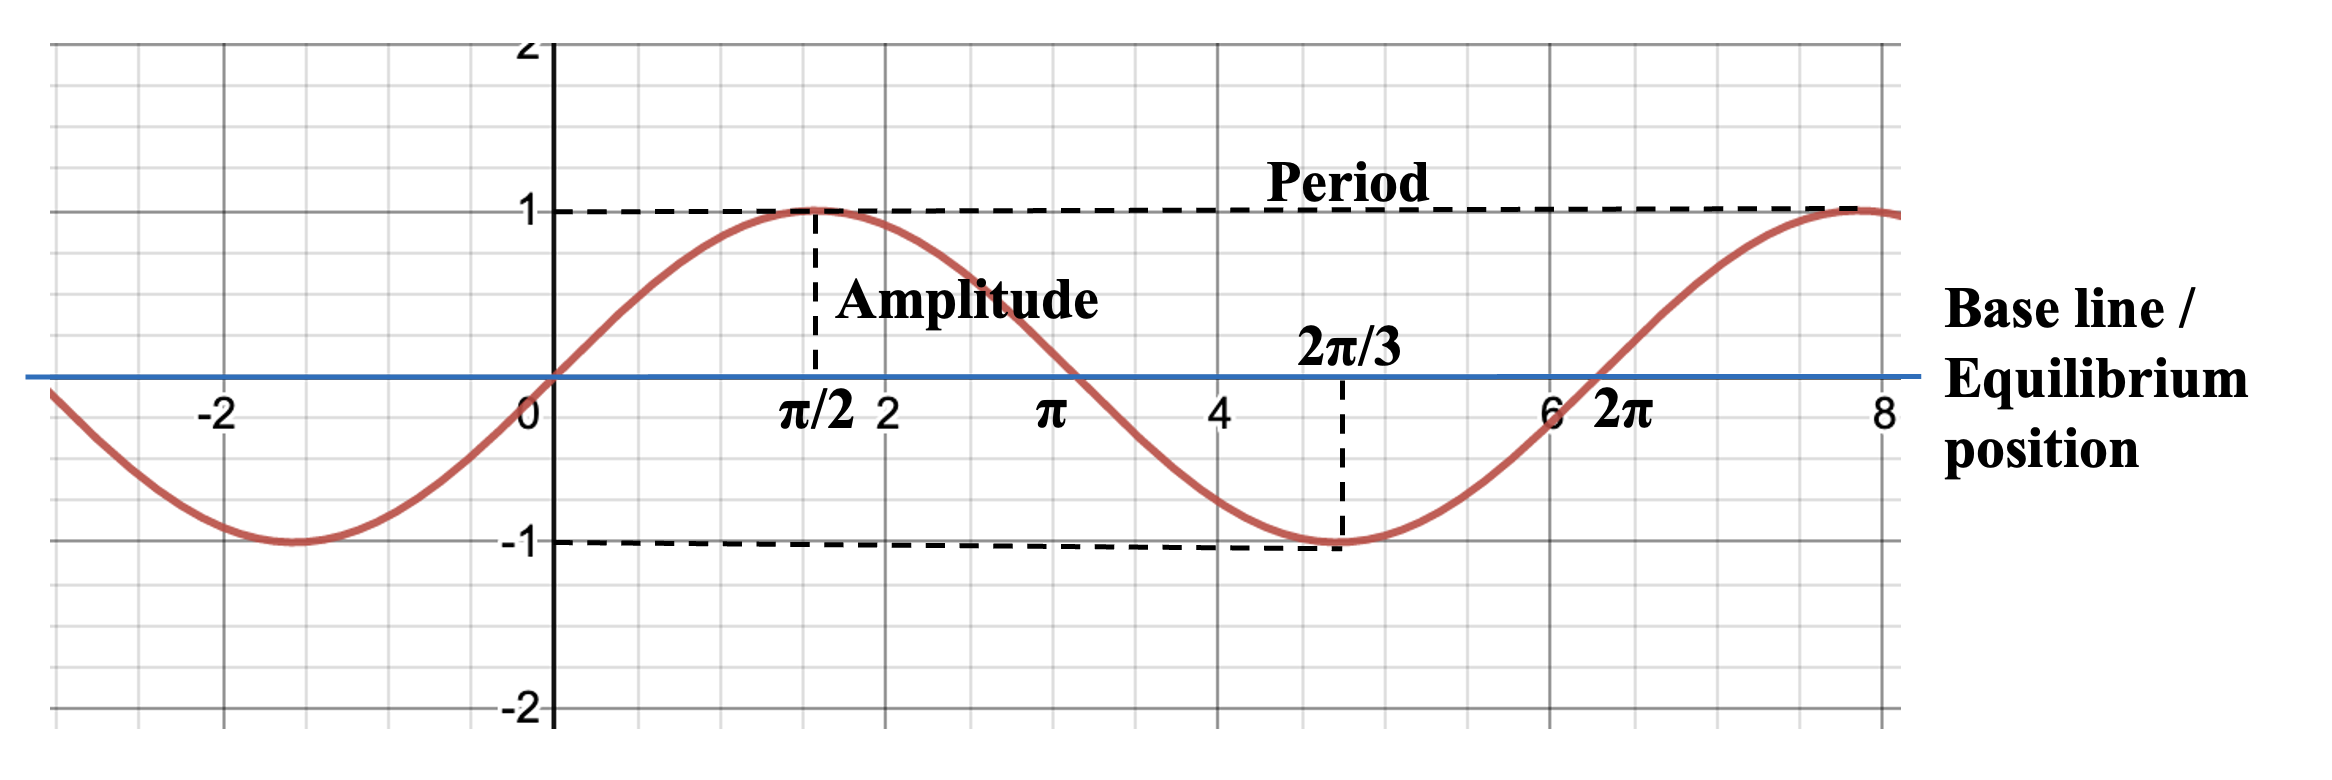
\includegraphics[width=0.9\textwidth]{Fig.3.25.jpg}
  \end{figure}
  $$\text{T(Period)}=2\pi;$$
  $$\text{Base line}=0;$$
  $$\text{Amplitude}=\left|\frac{y_{\text{max}}-y_{\text{min}}}{2}\right|=1;$$
  $$\text{Range: }\sin{x}\in\left[-1,\ 1\right];$$
  $$\text{Domain: }x\in\R.$$
  \item Cosine: Even function: $\cos{(-x)}=\cos{x}$.
  \begin{figure}[H]
    \centering
    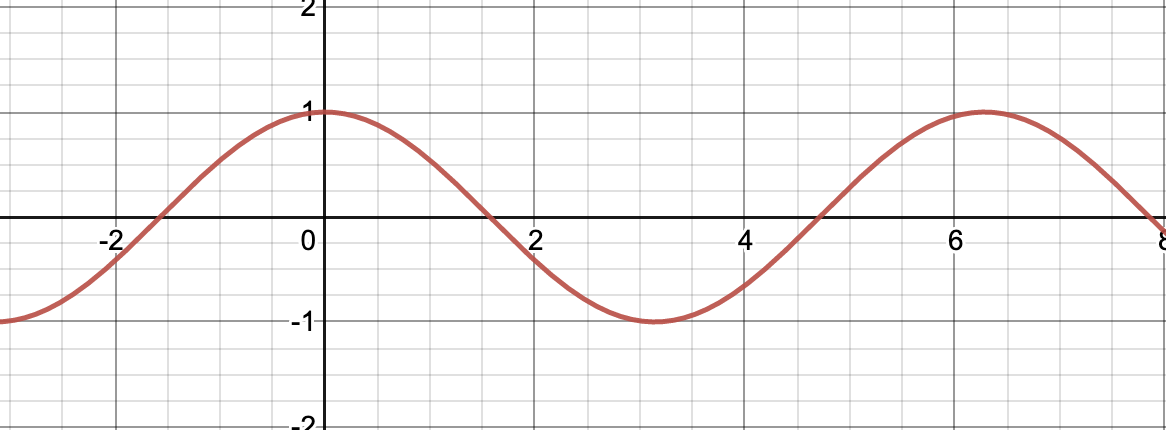
\includegraphics[width=0.85\textwidth]{Fig.3.26.jpg}
  \end{figure}
  $$\text{T(Period)}=2\pi;$$
  $$\text{Base line}=0;$$
  $$\text{Amplitude}=\left|\frac{y_{\text{max}}-y_{\text{min}}}{2}\right|=1;$$
  $$\text{Range: }\cos{x}\in\left[-1,\ 1\right];$$
  $$\text{Domain: }x\in\R.$$
  \item Tangent: 
  \begin{figure}[H]
    \centering
    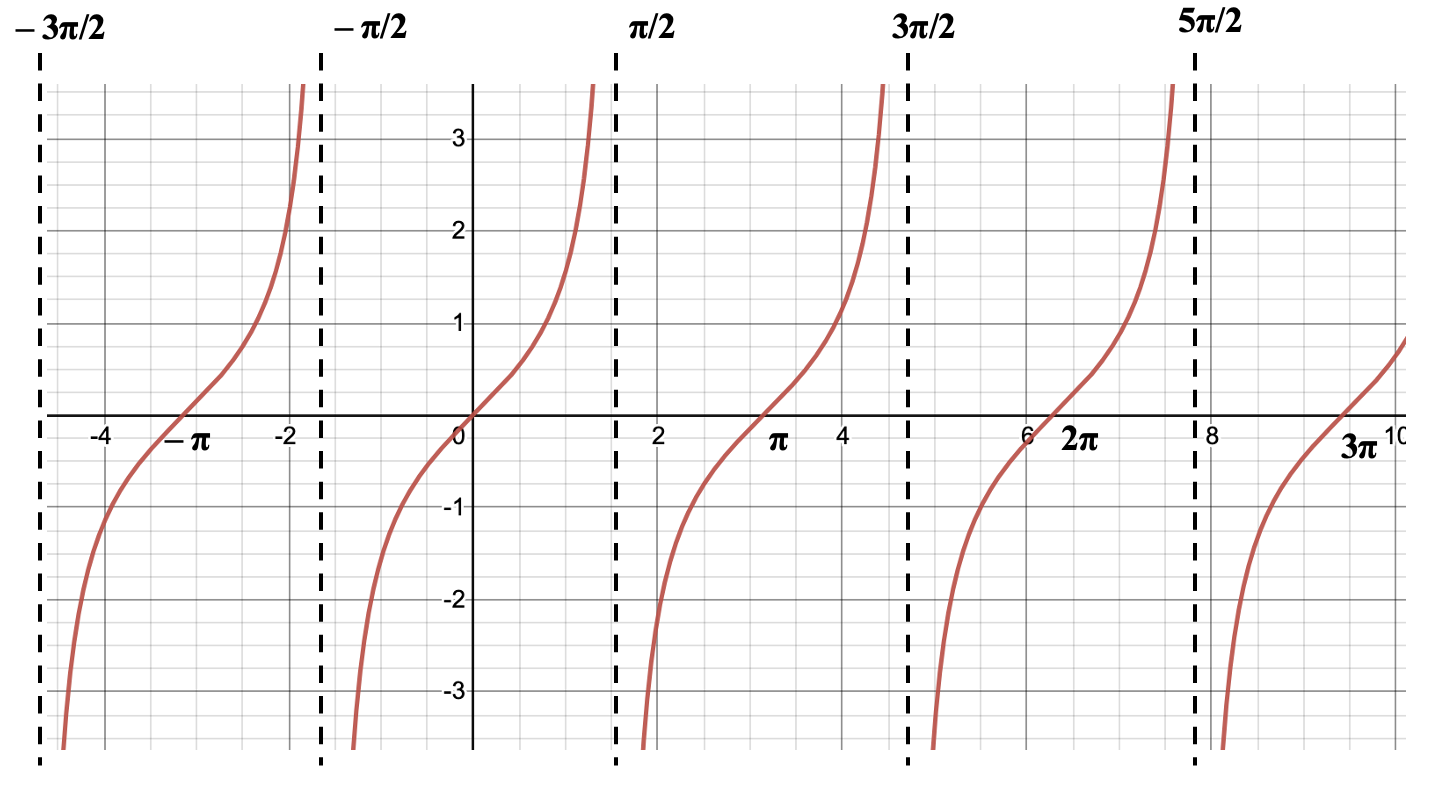
\includegraphics[width=0.9\textwidth]{Fig.3.27.jpg}
  \end{figure}
  $$\text{T(Period)}=\pi;$$
  $$\text{No amplitude(A)};$$
  $$\text{V.A.: }x=\frac{\pi}{2}+k\pi,\ k\in\Z;$$
  $$\text{Range: }\tan{x}\in\R;$$
  $$\text{Domain: }x\neq\frac{\pi}{2}+k\pi,\ k\in\Z.$$
  \item Transformation of Sine and Cosine: 
  $${\color{red}{y=A\sin{\left(\omega(x-\varphi)\right)}+h}}.$$
  \begin{itemize}
      \item Horizontal stretch with the scale factor of $\frac{1}{\omega}.\ \Rightarrow\ {\color{red}{\text{changes }T=\frac{\pi}{\omega}}}.$
      \item Horizontal translate to the right $\varphi$ units. $\Rightarrow$ {\color{red}{changes the initial point to $(\varphi, 0)$}}.
      \item Vertical stretch with a scale factor of $A$. $\Rightarrow$ {\color{red}{changes the amplitude$=|A|$}}. 
      \item Vertical translation of $h$ units upwards. $\Rightarrow$ {\color{red}{changes the equilibrium position $y=h$}}.
      \item Range of $y=A\sin{\left(\omega(x-\varphi)\right)}+h$: $y\in\left[h-A, h+A\right]$.
  \end{itemize}
  $${\color{red}{y=A\cos\left(\omega(x-\varphi)\right)+h}}.$$
  \begin{itemize}
    \item Horizontal stretch with the scale factor of $\frac{1}{\omega}.\ \Rightarrow\ {\color{red}{\text{changes }T=\frac{\pi}{\omega}}}.$
    \item Horizontal translate to the right $\varphi$ units. $\Rightarrow$ {\color{red}{changes the initial point to $(\varphi, 1)$}}.
    \item Vertical stretch with a scale factor of $A$. $\Rightarrow$ {\color{red}{changes the amplitude$=|A|$, initial point $(\varphi, A)$}}. 
    \item Vertical translation of $h$ units upwards. $\Rightarrow$ {\color{red}{changes the equilibrium position $y=h$, initial point $(\varphi, A+h)$}}.
  \end{itemize}
  \item Cotangent: 
  \begin{figure}[H]
    \centering
    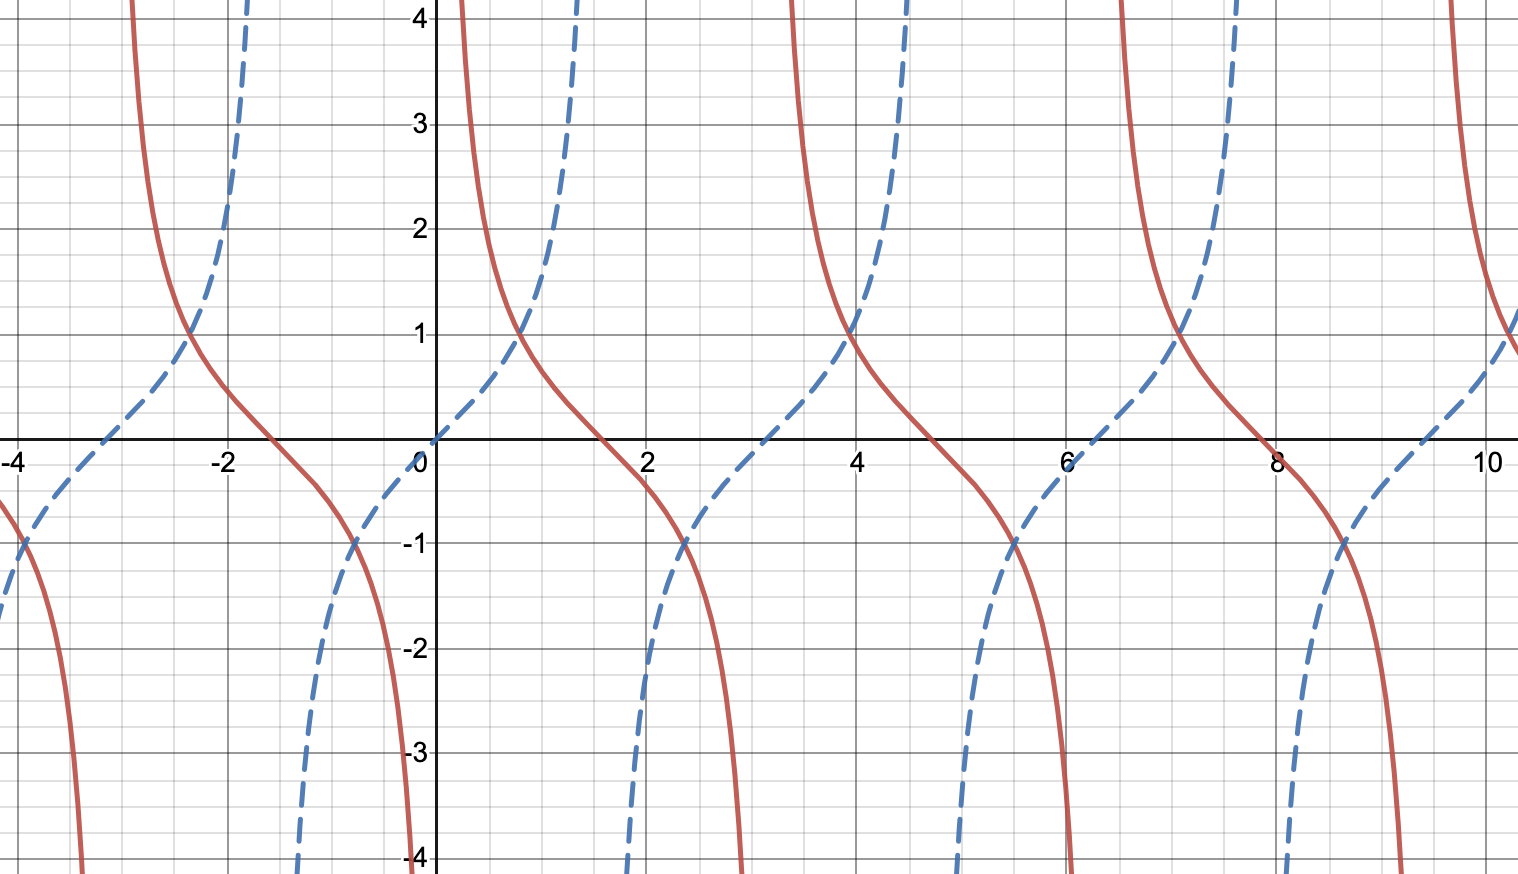
\includegraphics[width=0.85\textwidth]{Fig.3.28.jpg}
  \end{figure}
  $$\text{V.A.: }x=k\pi$$
  $$\text{Period: }\pi$$
  $$\text{Pass through}\left(\frac{\pi}{2}+k\pi, 0\right)$$
  \item Cosecant: 
  \begin{figure}[H]
    \centering
    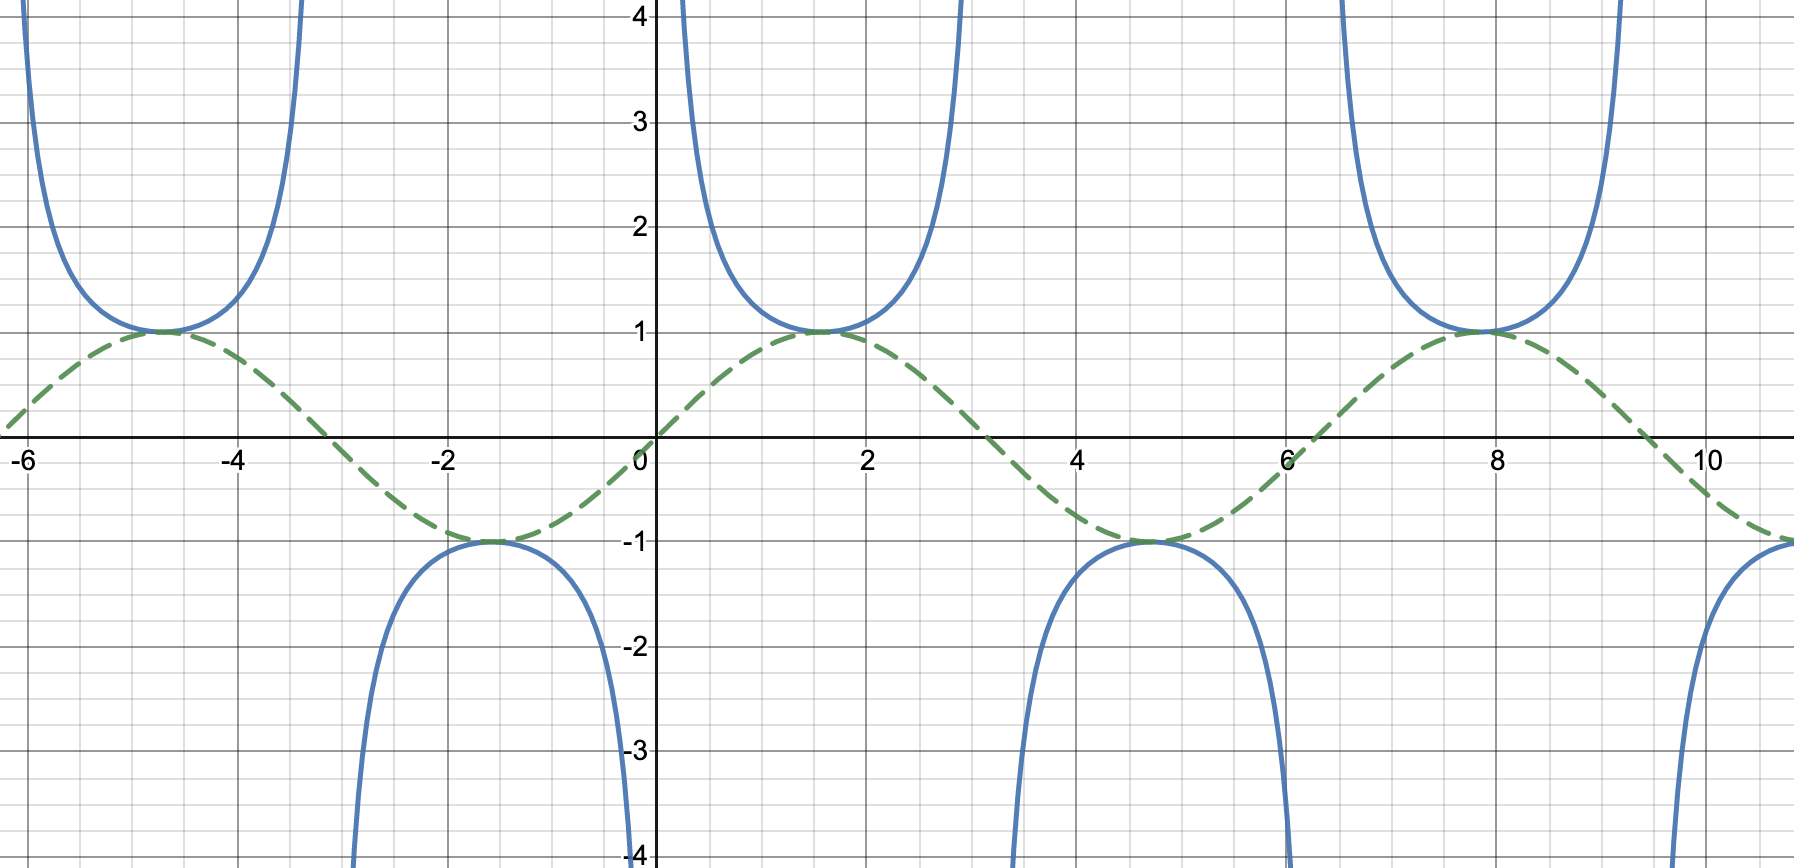
\includegraphics[width=0.85\textwidth]{Fig.3.29.jpg}
  \end{figure}
  $$\text{Domain: }x\neq k\pi$$
  $$\text{Range: }y\in\left.\right]-\infty,-1\left[\right.\cup\left.\right]1,+\infty\left[\right.$$
  \item Secant: 
  \begin{figure}[H]
    \centering
    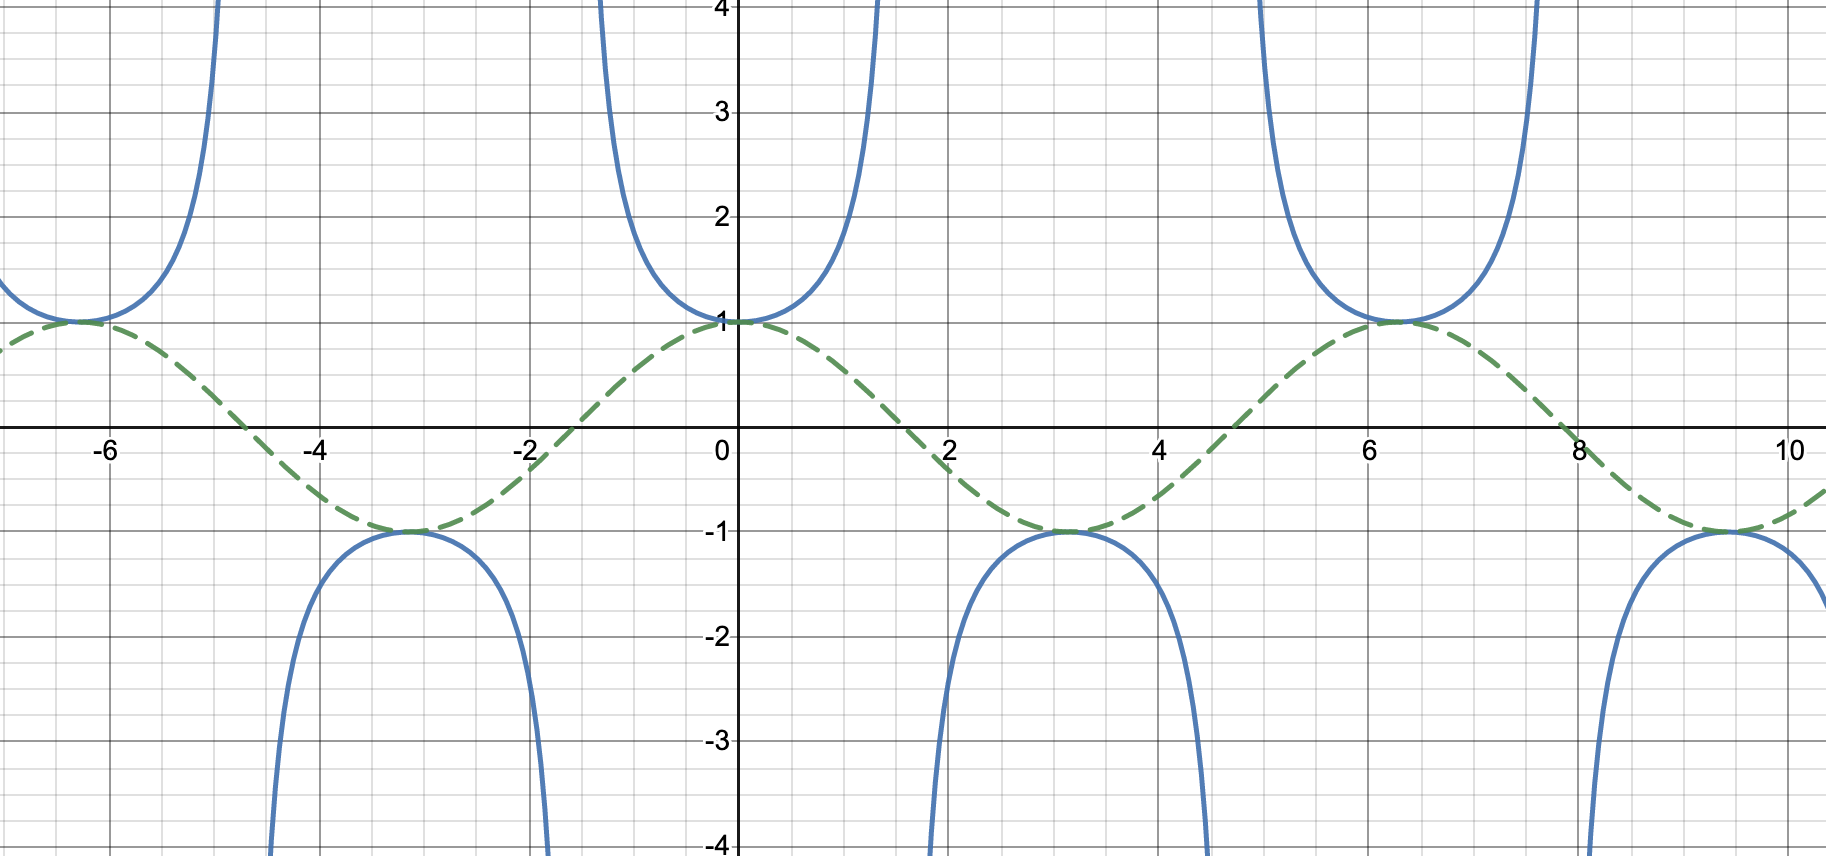
\includegraphics[width=0.85\textwidth]{Fig.3.30.jpg}
  \end{figure}
  $$\text{Domain: }x\neq\frac{\pi}{2}+k\pi$$
  $$\text{Range: }y\in\left.\right]-\infty,-1\left[\right.\cup\left.\right]1,+\infty\left[\right.$$
  \item When drawing the graph of $sec{x}$ and $\csc{x}$, draw $cos{x}$ and $\sin{x}$ first. 
  \item Conversion between sine and cosine: 
  \begin{itemize}
    \item $$\sin{\left(\frac{\pi}{2}-x\right)}=\cos{x}$$
    \item $$\cos{\left(\frac{\pi}{2}-x\right)}=\sin{x}$$
    \item $$\cos{\left(\frac{\pi}{2}+x\right)}=\cos\left[\pi-\left(\frac{\pi}{2}-x\right)\right]=-\cos{\left(\frac{\pi}{2}-x\right)}=-\sin{x}$$
    \item $$\sin{\left(\frac{\pi}{2}+x\right)}=\sin\left[\pi-\left(\frac{\pi}{2}-x\right)\right]=\sin{\left(\frac{\pi}{2}-x\right)}=\cos{x}$$
  \end{itemize}
\end{enumerate}

\subsubsection{Solving Trigonometric Functions}
\begin{enumerate}
  \item Solving Trigonometric Functions in Paper 1: 
  \begin{itemize}
    \item Values of sepcial angles
    \item From relative acute angles and CAST rule
    \item Modification of period
    \item Check the solution with domain
  \end{itemize}
  \begin{example}
    \textbf{Solve for $\cos{x}=\frac{\sqrt{3}}{2}$ for $0<x<3\pi$.}
    $$\text{Consider }x\in[0,2\pi]$$
    $$x=\frac{\pi}{6}, \frac{11\pi}{6}.$$
    $$\text{In the domain of }x\in[0,3\pi],$$
    $$\text{Another solution is }\frac{13\pi}{6}.$$
  \end{example}
  \item Transformed Trigonometric Equations: 
  \begin{example}
    \textbf{Solve $6\sin\left(2\left(x-\frac{\pi}{6}\right)\right)-2=1,\ \frac{\pi}{6}<x<2\pi$.}
    $$\sin\left(2\left(x-\frac{\pi}{6}\right)\right)=\frac{1}{2}.$$
    $$\text{Let }t=2\left(x-\frac{\pi}{6}\right):$$
    $$\because \frac{\pi}{6}<x<2\pi, $$
    $$\therefore 0<2\left(x-\frac{\pi}{6}\right)<\frac{11\pi}{3},\ 0<t<\frac{11\pi}{3}.$$
    $$\sin t=\frac{1}{2}\ \Rightarrow\ t=\frac{\pi}{6},\ \frac{5\pi}{6},\ \frac{13\pi}{6},\ \frac{17\pi}{6};$$
    $$\Rightarrow x=\frac{\pi}{4},\ \frac{7\pi}{12},\ \frac{5\pi}{4},\ \frac{19\pi}{12}.$$
  \end{example}
  \item Solving Trigonometric Functions in Paper 2: 
  \begin{itemize}
    \item Change mode to RADIAN.
    \item Plot the functions. 
    \item Adjust the window. 
    \item Calculate the intersects.
    \item Repeat step 4 if necessary. 
  \end{itemize}
\end{enumerate}

\subsubsection{Inverse Trigonometric Functions}
\begin{enumerate}
  \item Inverse Trigonometric Function: 
  \begin{itemize}
    \item $$y=\arcsin{x}$$
    \item $$y=\arccos{x}$$
    \item $$y=\arctan{x}$$
    \item $$\text{arcsec}x=\arccos{\left(\frac{1}{x}\right)}$$
    \item $$\text{arccsc}x=\arcsin{\left(\frac{1}{x}\right)}$$
    \item $$\text{arccot}x=\arctan{\left(\frac{1}{x}\right)}$$
  \end{itemize}
  \item One-to-one Function: 
  \begin{itemize}
    \item In order for functions to have the inverse function, it must be so called \textbf{\color{red}{one-to-one}} function (bijection). 
    \item One $x$ value to one (and only one) $y$ value.\\
    One $y$ value to one (and only one) $x$ value. 
  \end{itemize}
  \item Domain and range for $\arcsin{x}$: 
  \begin{itemize}
    \begin{figure}[H]
      \centering
      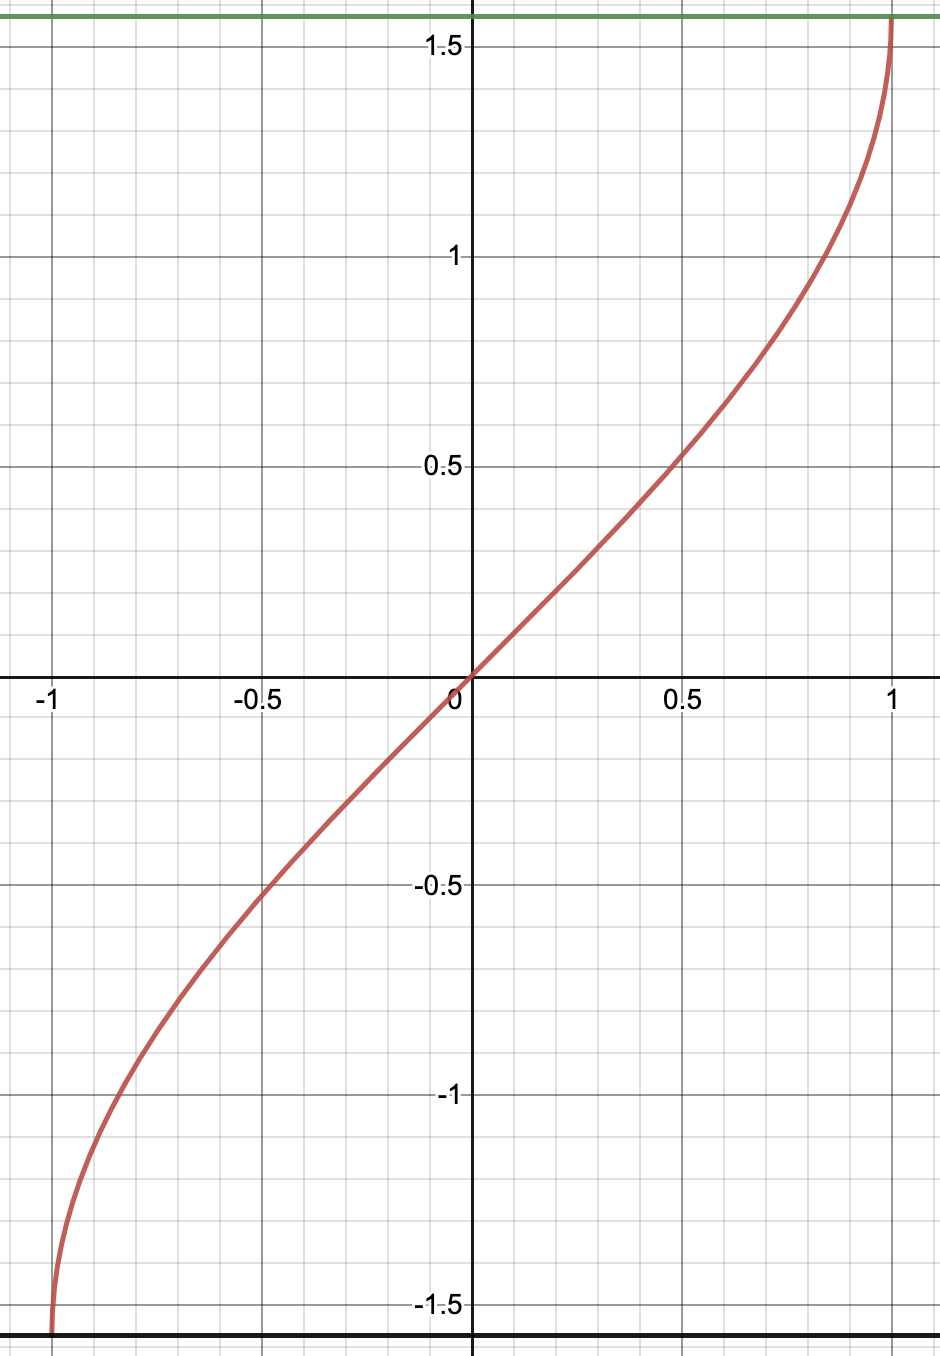
\includegraphics[width=0.45\textwidth]{Fig.3.31.jpg}
    \end{figure}
    \item Domain: $x\in\left[-1,1\right]$ {\color{green}{(Range $\sin{x}\in\left[-1,1\right]$)}}.
    \item Range: $\arcsin{x}\in\left[-\frac{\pi}{2},\frac{\pi}{2}\right]$ {\color{green}{(Domain $\sin{x}\in\left[-\frac{\pi}{2},\frac{\pi}{2}\right]$)}}.
  \end{itemize}
  \item Domain and range for $\arccos{x}$:
  \begin{itemize}
  \begin{figure}[H]
    \centering
    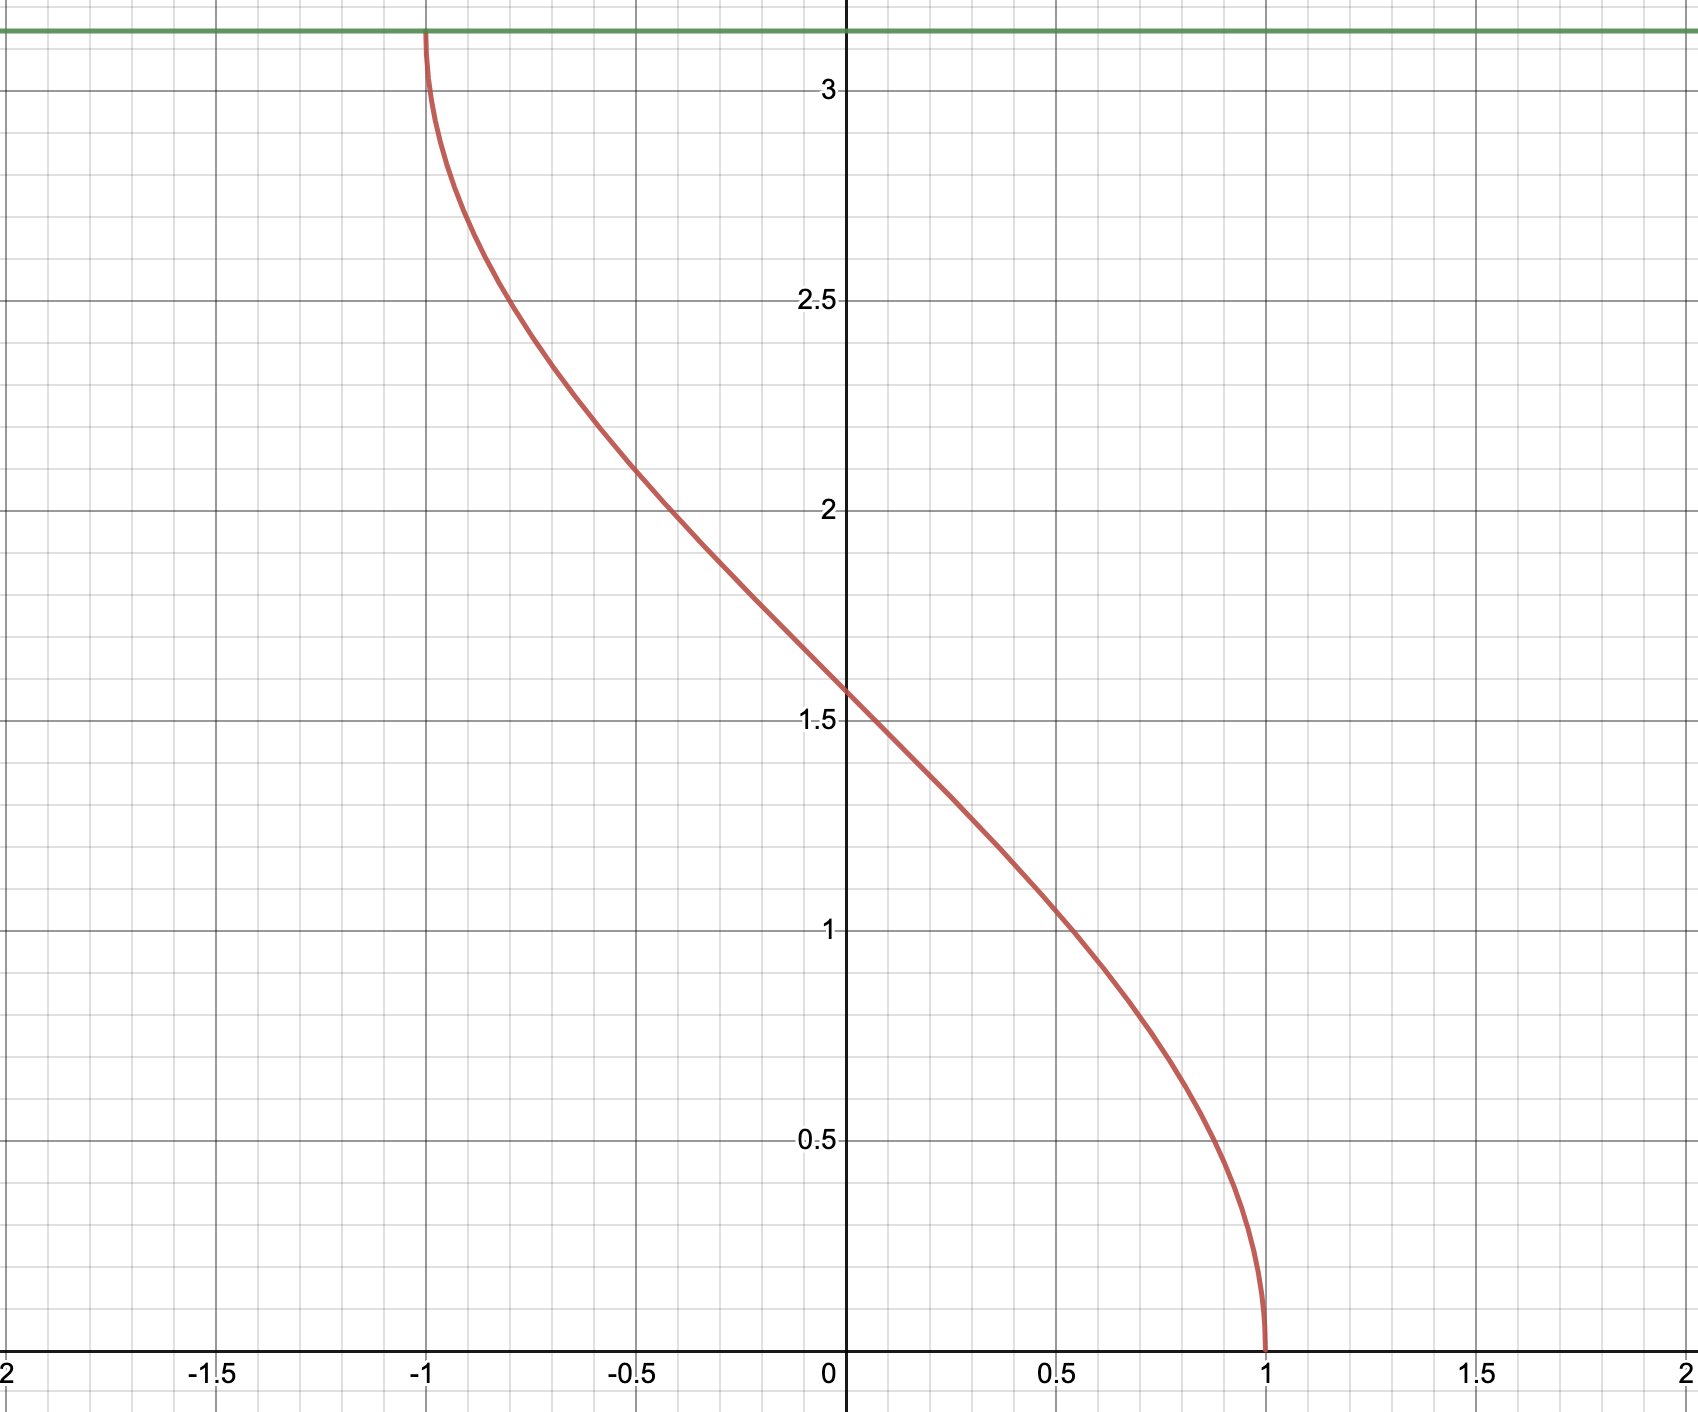
\includegraphics[width=0.6\textwidth]{Fig.3.32.jpg}
  \end{figure}
  \item Domain: $x\in\left[-1,1\right]$.
  \item Range: $\arccos{x}\in\left[0,\pi\right]$.
  \end{itemize}
  \item Domain and range for $\arctan{x}$: 
  \begin{itemize}
  \begin{figure}[H]
    \centering
    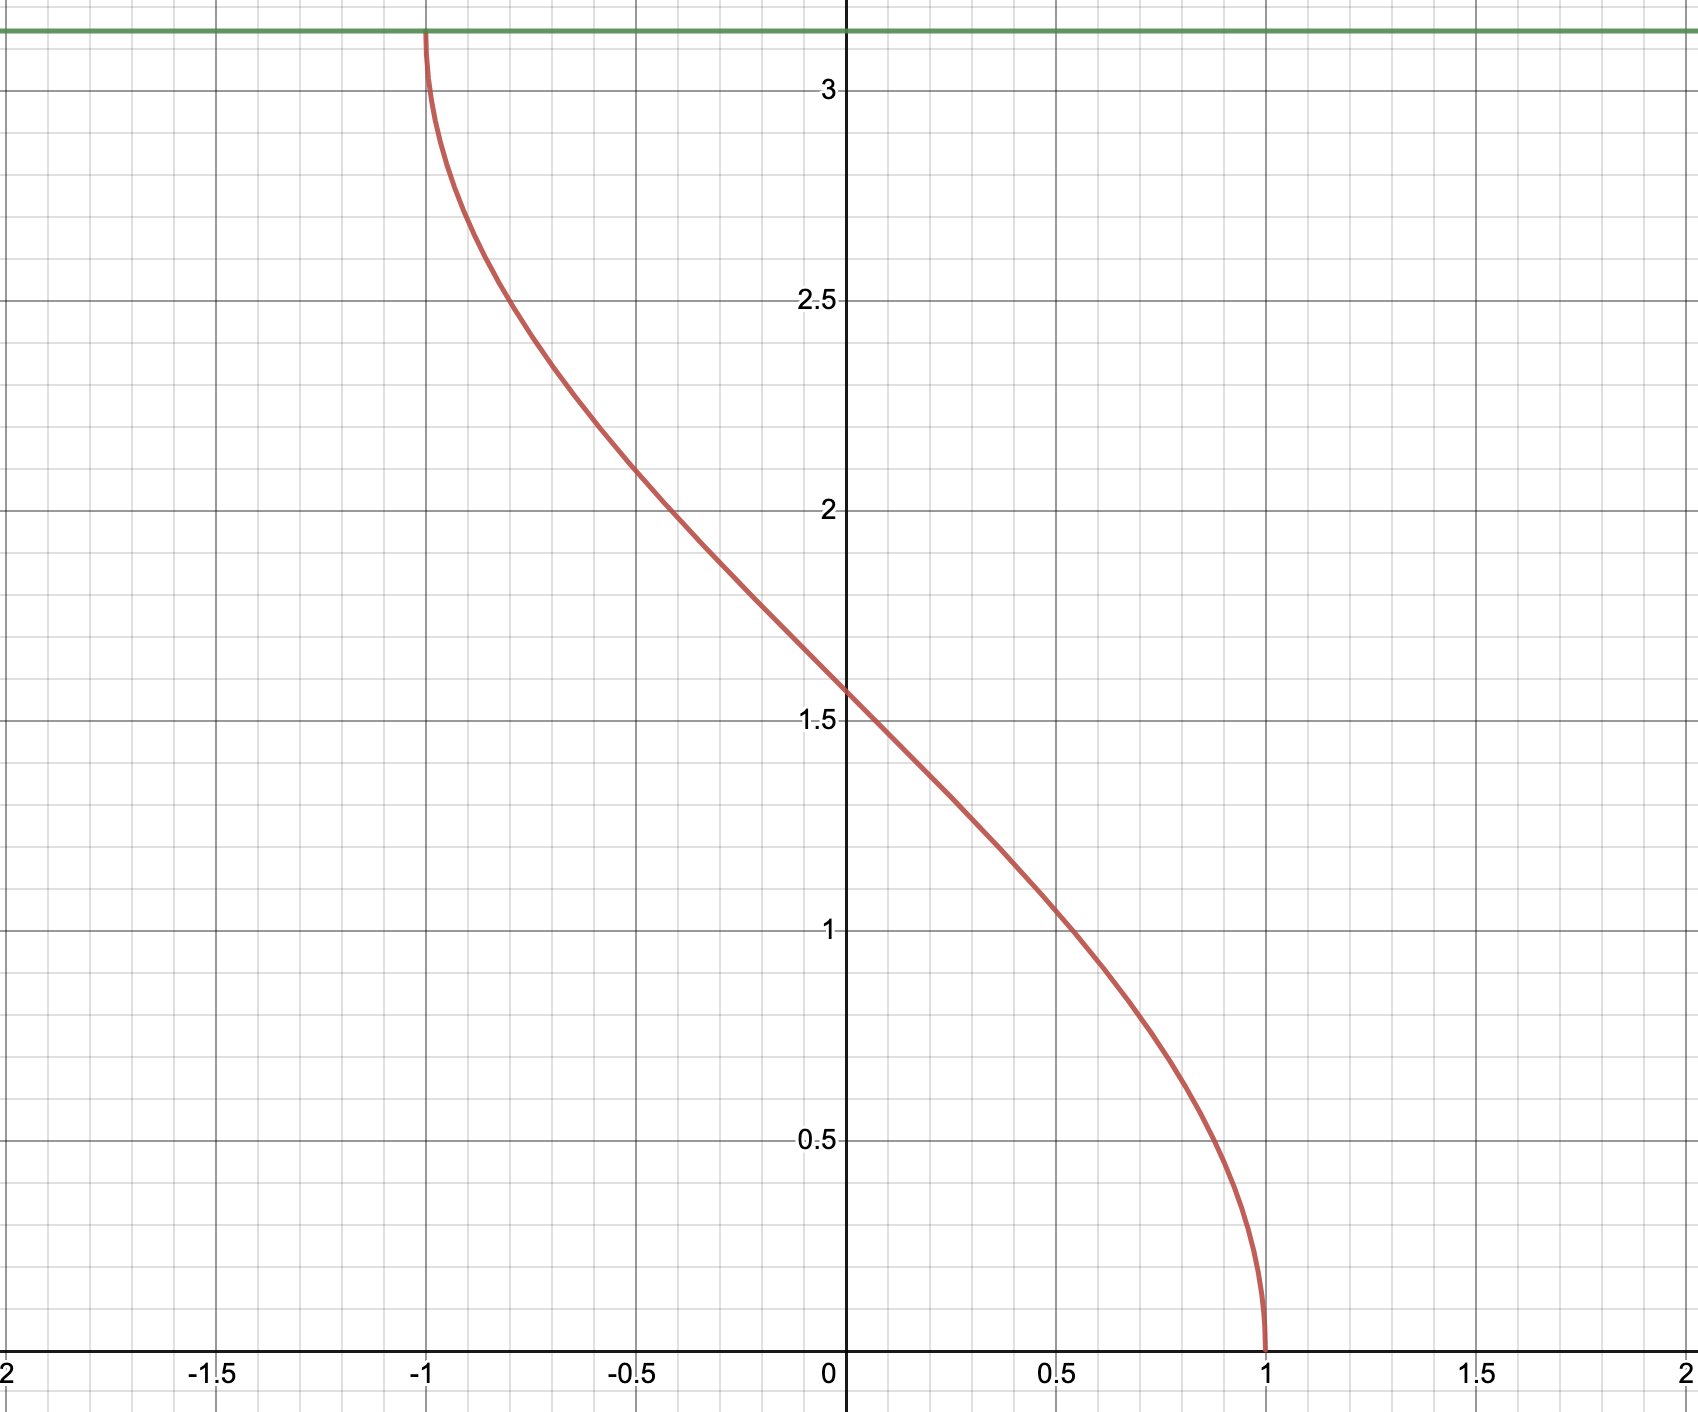
\includegraphics[width=0.6\textwidth]{Fig.3.32.jpg}
  \end{figure}
  \item Domain: $x\in\R$
  \item Range: $y\in\left.\right]-\frac{\pi}{2},\frac{\pi}{2}\left[\right.$
  \end{itemize}
\end{enumerate}

\subsection{Vectors}
\subsubsection{Introduction to Vectors}
\begin{enumerate}
  \item Vector: 
  \begin{definition}
    A \textbf{\color{red}{vector}} is a quantity with a direction and magnitude. It is noted as {\color{red}{$\vec{a}$}}.
  \end{definition}
  \item Components of a vector: 
  \begin{itemize}
    \item 2-D: 
    \begin{figure}[H]
      \centering
      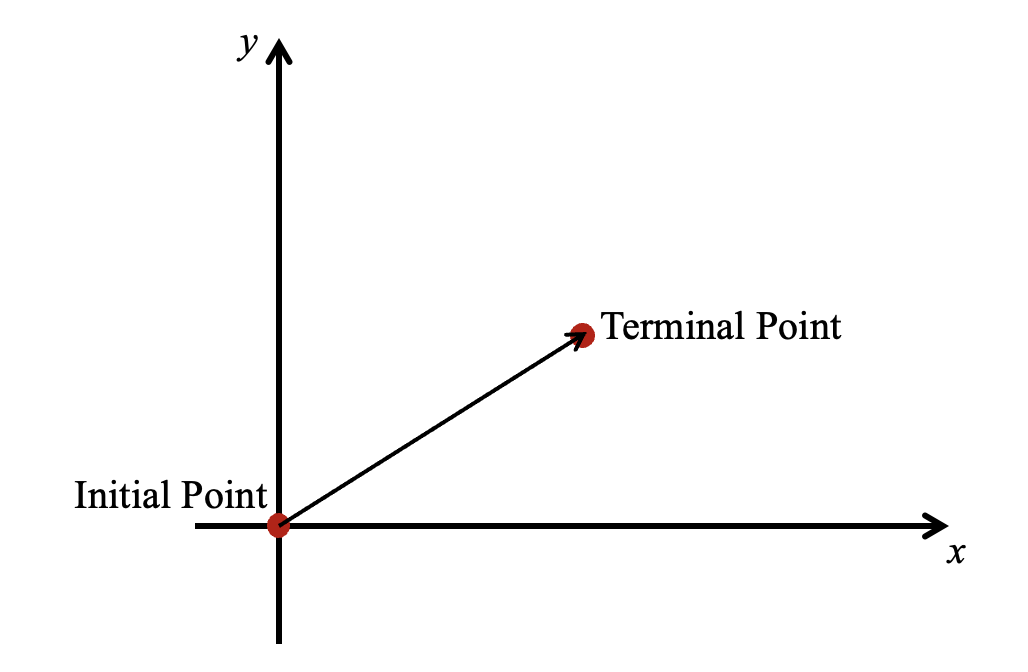
\includegraphics[width=0.5\textwidth]{Fig.3.1.jpg}
    \end{figure}
    \begin{example}
      The vector $\vec{a}=\binom{3}{2}$ menas 3 units in the horizontal direction and 2 units in the vertical direction.
    \end{example}
    \item 3D: 
    \begin{figure}[H]
      \centering
      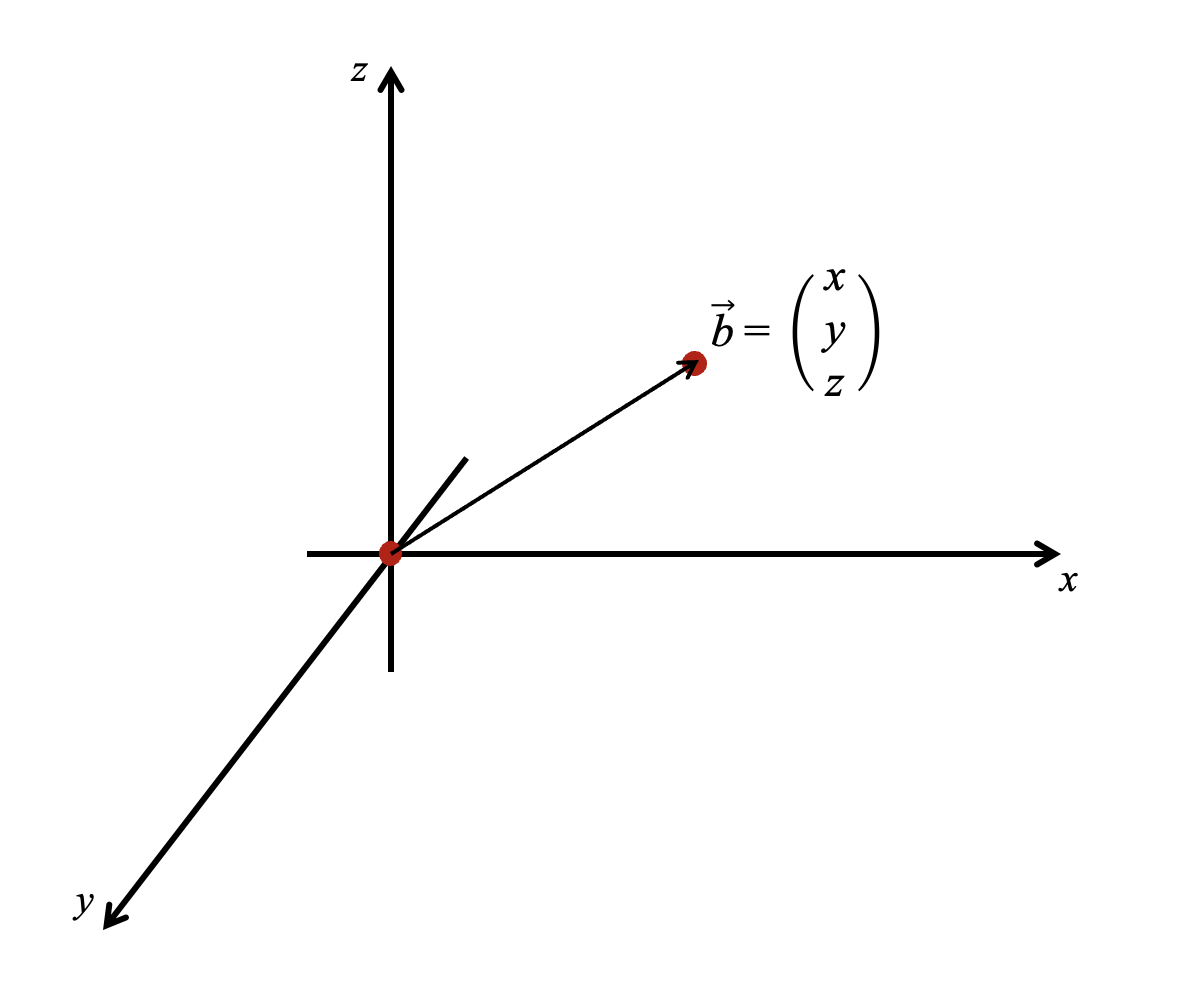
\includegraphics[width=0.5\textwidth]{Fig.3.2.jpg}
    \end{figure}
  \end{itemize}
  \item \textbf{\color{red}{Magnitude/Modulus}} of vector: 
  \begin{itemize}
    \item 2D: $$\text{For }\vec{a}=\begin{pmatrix}x\\y\end{pmatrix},\ {\color{red}{\left|\vec{a}\right|=\sqrt{x^2+y^2}}}.$$
    \item 3D: $$\text{For }\vec{b}=\begin{pmatrix}x\\y\\z\end{pmatrix},\ {\color{red}{\left|\vec{b}\right|=\sqrt{x^2+y^2+z^2}}}.$$
  \end{itemize}
  \item \textbf{\color{red}{Unit Vector}}: A vector of length 1: 
  \begin{itemize}
    \item $\vec{i}$: unit vector on the $x$-axis.
    \item $\vec{j}$: unit vector on the $y$-axis.
    \item $\vec{k}$: unit vector on the $z$-axis.
    \begin{figure}[H]
      \centering
      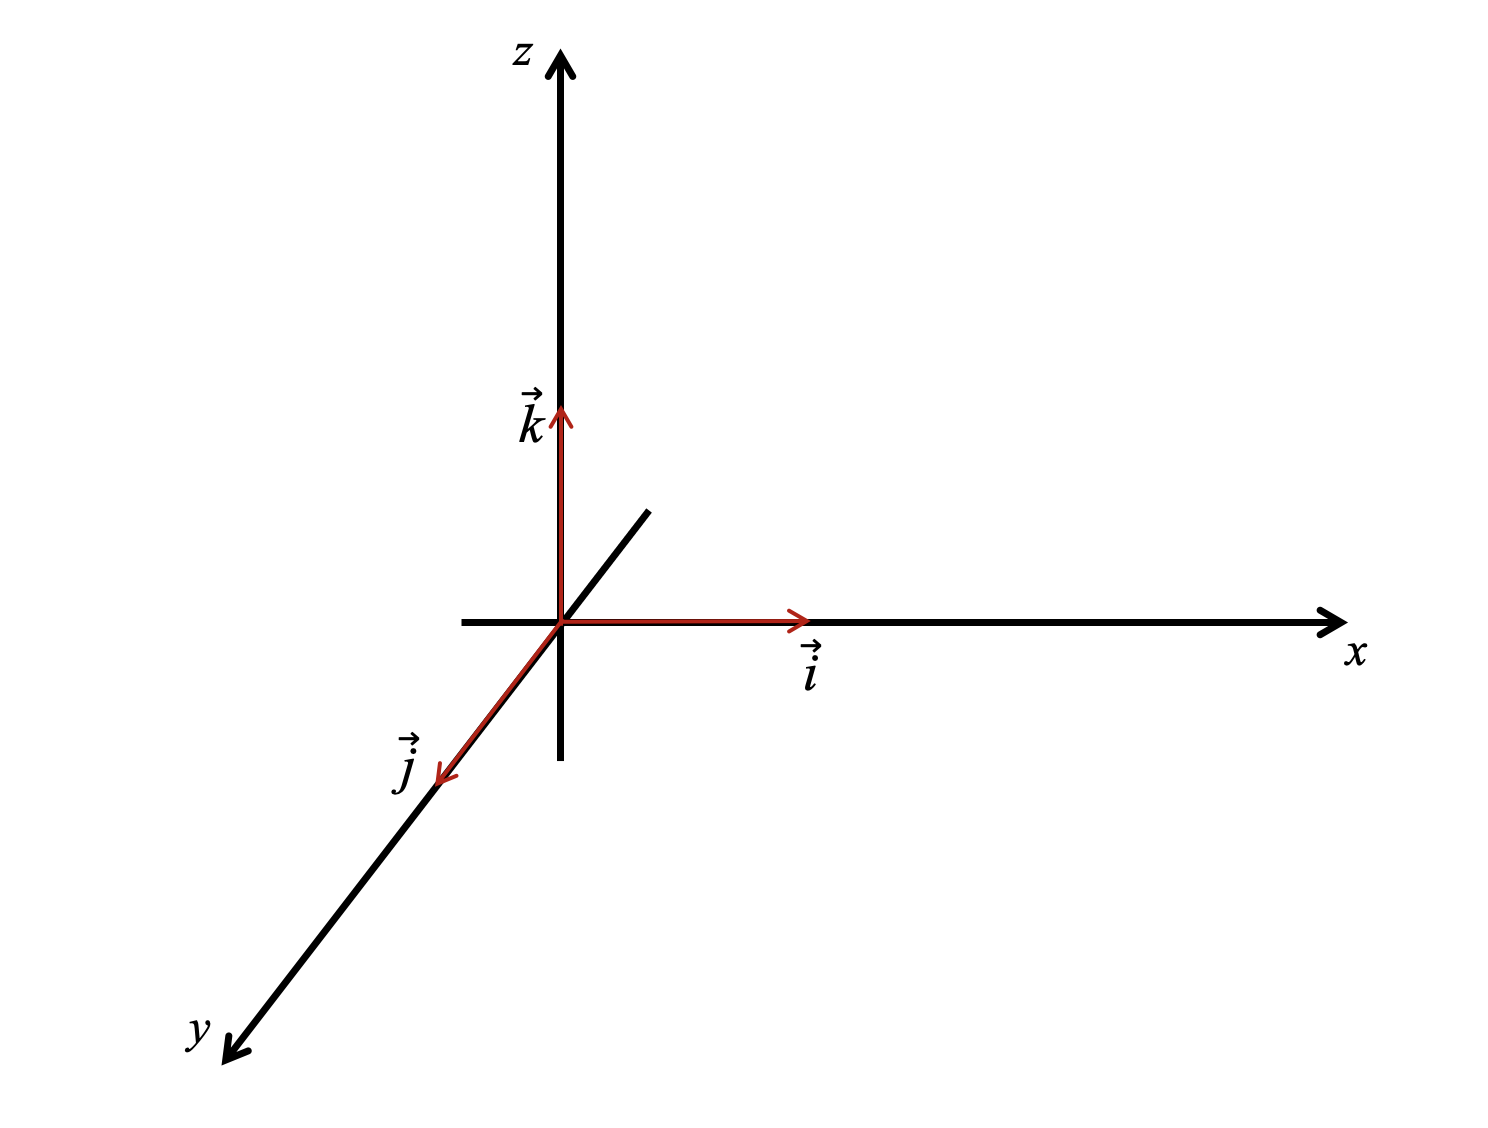
\includegraphics[width=0.5\textwidth]{Fig.3.3.jpg}
    \end{figure}
  \end{itemize}
  \item Sum of vectors: 
  \begin{itemize}
    \item \textbf{\color{red}{Position vector}}: A vector that has an initial point at the origin. 
    \begin{example}
      $$\vec{a}=\begin{pmatrix}3\\2\end{pmatrix}$$
      $$\vec{a}=3\vec{i}+2\vec{j}.$$
      \begin{figure}[H]
        \centering
        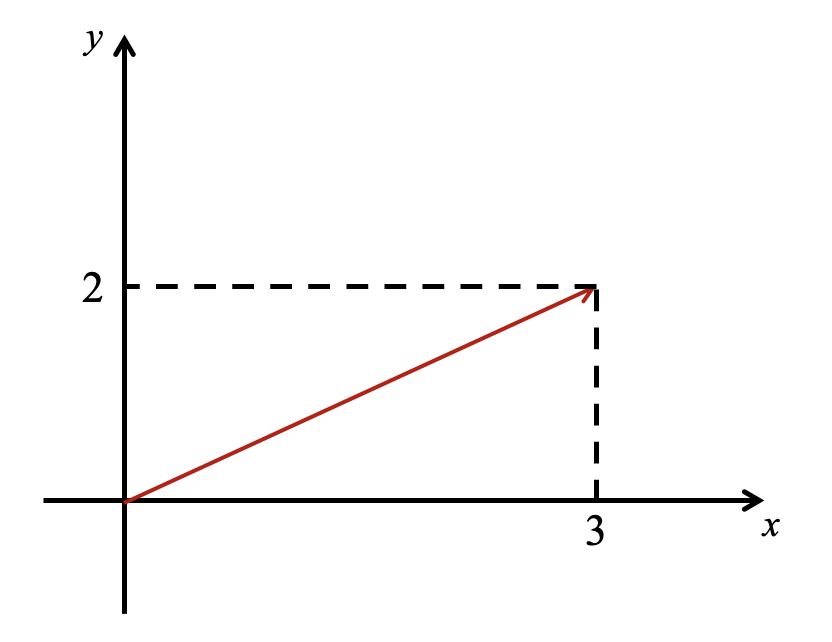
\includegraphics[width=0.5\textwidth]{Fig.3.4.jpg}
      \end{figure}
    \end{example}
    \item Let $\vec{a}=\begin{pmatrix}x\\y\end{pmatrix}$ and $\vec{b}=\begin{pmatrix}m\\n\end{pmatrix}$
    $${\color{red}{\vec{a}+\vec{b}=\begin{pmatrix}x+m\\y+n\end{pmatrix}}}.$$
  \end{itemize}
  \item Multiplication of vectors by a scalar: \\
  Let $\vec{a}=\begin{pmatrix}x\\y\end{pmatrix}$ and $n$ be a scalar: 
  $${\color{red}{n\vec{a}=n\begin{pmatrix}x\\y\end{pmatrix}=\begin{pmatrix}nx\\ny\end{pmatrix}}}.$$
  {\color{green}{$n\vec{a}$ and $\vec{a}$ are in the same direction $\Rightarrow$ parallel.}}
  \item Subtracting a vector: \\
  Let $\vec{a}=\begin{pmatrix}x\\y\end{pmatrix}$, $\vec{b}=\begin{pmatrix}m\\n\end{pmatrix}$.
  $${\color{red}{\vec{a}-\vec{b}=\begin{pmatrix}x-m\\y-n\end{pmatrix}}}.$$
  \begin{proof}
    $$\begin{aligned}
      -\vec{b}&=(-1)\vec{b}=\begin{pmatrix}-m\\-n\end{pmatrix}\\
      \vec{a}-\vec{b}&=\vec{a}+\left(-\vec{b}\right)=\begin{pmatrix}x-m\\y-n\end{pmatrix}.
    \end{aligned}$$
  \end{proof}
  \item \textbf{\color{red}{Zero vector}}: $\vec{0}$.
  \item \textbf{\color{red}{Collinear points}}: three points, $A$, $B$, and $C$, are said to be collinear if ${\color{red}{\vec{AB}=t\vec{AC}}}$.
  \begin{figure}[H]
    \centering
    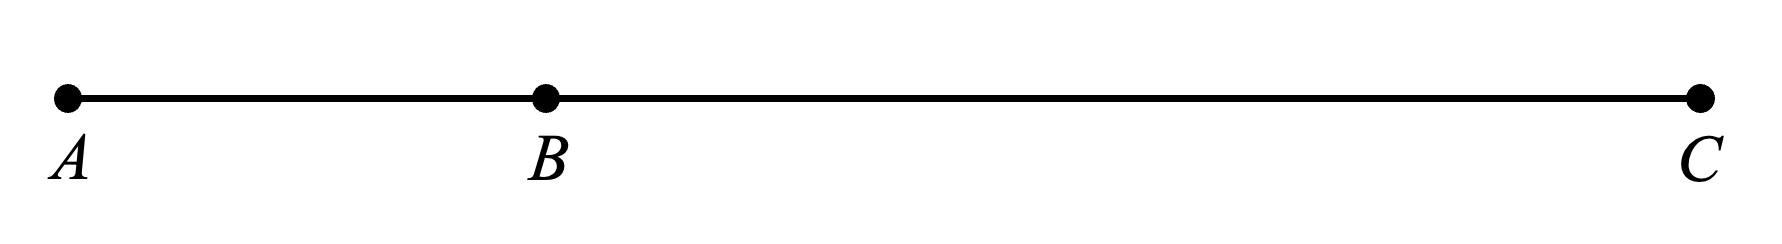
\includegraphics[width=0.5\textwidth]{Fig.3.5.jpg}
  \end{figure}
  \item Find a unit vector parralel to $\vec{u}=\begin{pmatrix}x\\y\end{pmatrix}.$
  \begin{itemize}
    \item Find the value $\left|\vec{u}\right|.$
    \item Then, the unit vector parralel to $\vec{u}$ is 
    $${\color{red}{\vec{v}=\frac{\vec{u}}{\left|\vec{u}\right|}}}.$$
  \end{itemize}
  \item Vectors and unit circle: 
  \begin{figure}[H]
    \centering
    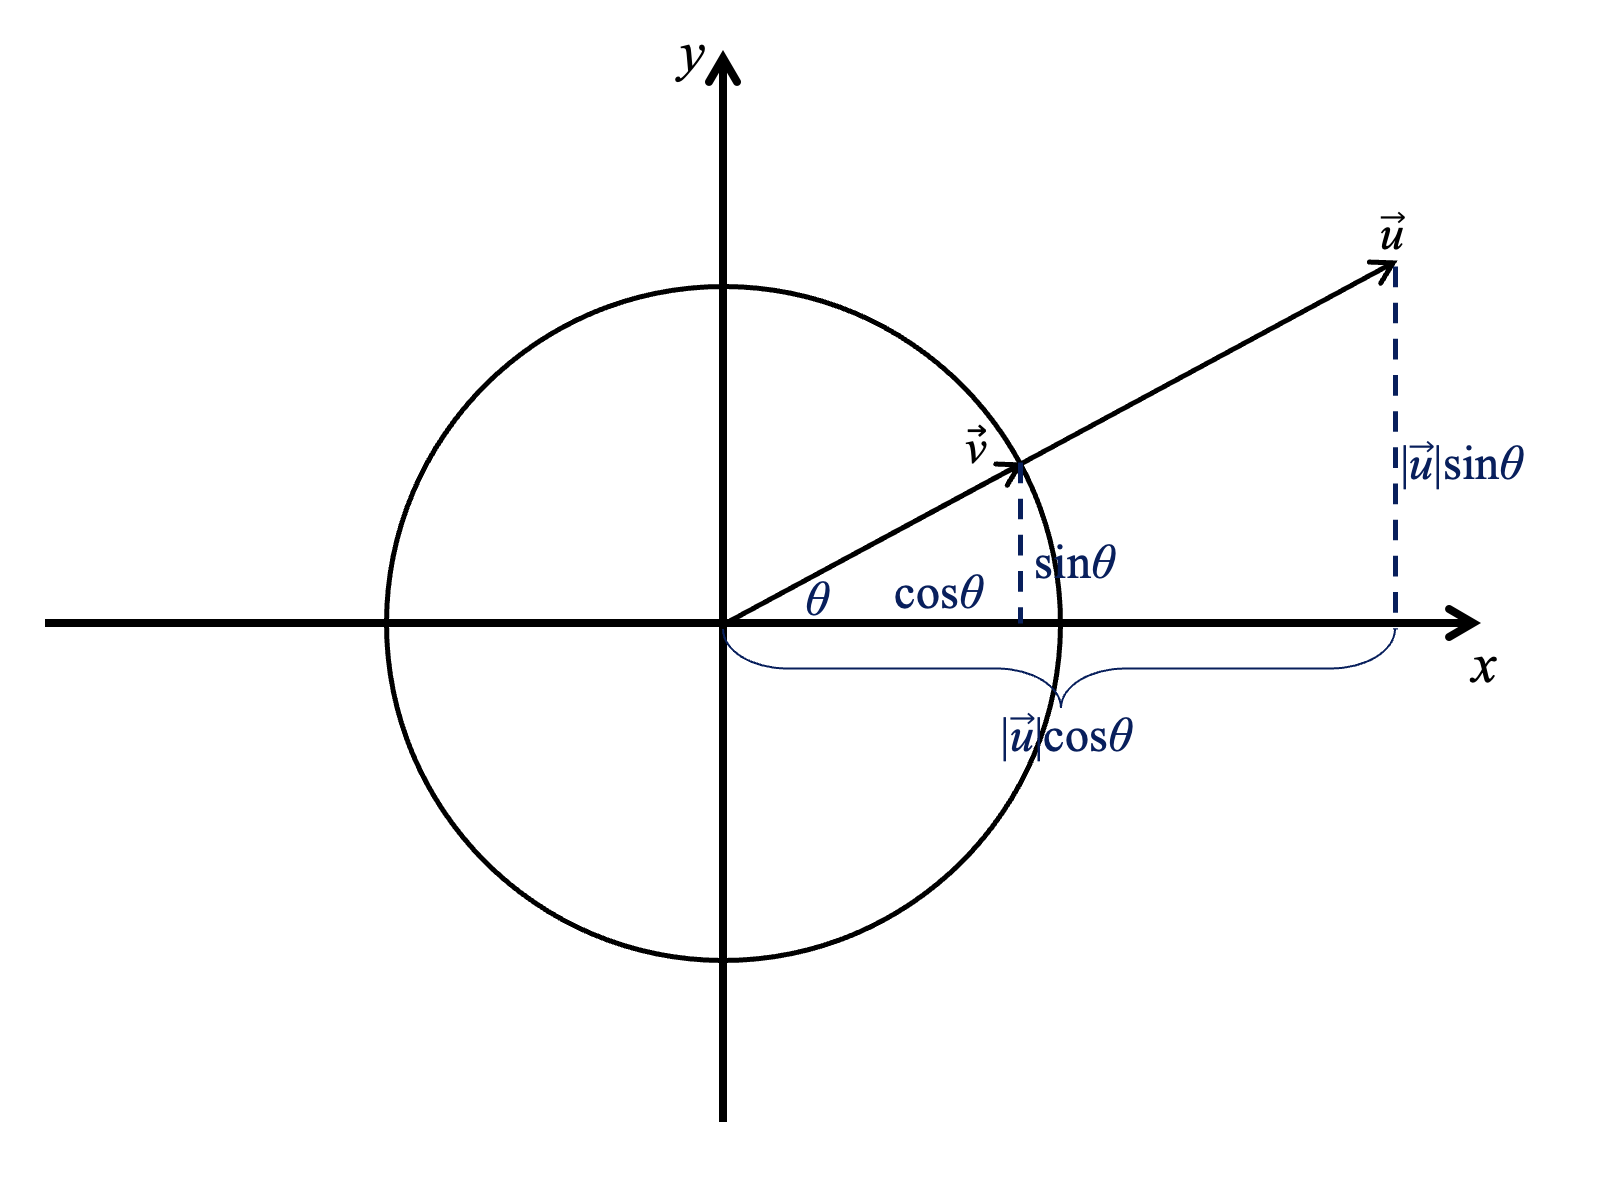
\includegraphics[width=0.5\textwidth]{Fig.3.6.jpg}
  \end{figure}
  $\theta$ is the angle with the horizontal axis. The unit vector $\vec{v}$, in the same direction as $\vec{u}$ is: 
  $$\vec{v}=\cos\theta\cdot\vec{i}+\sin\theta\cdot\vec{j}\\$$
  $$\begin{aligned}
    \vec{v}=\frac{1}{\left|\vec{u}\right|}\cdot\vec{u}\ \Rightarrow\ \vec{u}=\left|\vec{u}\right|\cdot\vec{v}&=\left|\vec{u}\right|\cos\theta\cdot\vec{i}+\left|\vec{u}\right|\sin\theta\cdot\vec{j}\\
    &=\left|\vec{u}\right|\left(\cos\theta\cdot\vec{i}+\sin\theta\cdot\vec{j}\right).
  \end{aligned}$$
\end{enumerate}

\subsubsection{Scalar Product and Its Properties}
\begin{enumerate}
  \item The \textbf{\color{red}{scalar product}} of two vectors is a real number (scalar). 
  \begin{itemize}
    \item The algebraic definition: \\
    For $\vec{a}=\begin{pmatrix}a_1\\a_2\end{pmatrix}$ and $\vec{b}=\begin{pmatrix}b_1\\b_2\end{pmatrix}$,
    $${\color{red}{\vec{a}\cdot\vec{b}=\begin{pmatrix}a_1\\a_2\end{pmatrix}\cdot\begin{pmatrix}b_1\\b_2\end{pmatrix}=a_1b_1+a_2b_2}}.$$
    {\color{green}{The scalar product is also called the dot product. }}
    \item The geometric definition: \\
    For $\vec{a}$ and $\vec{b}$,
    $${\color{red}{\vec{a}\cdot\vec{b}=\left|\vec{a}\right|\left|\vec{b}\right|\cos\theta}},\ \theta{\text{is the angle between the two vectors.}}$$
    \begin{proof}
      \begin{figure}[H]
        \centering
        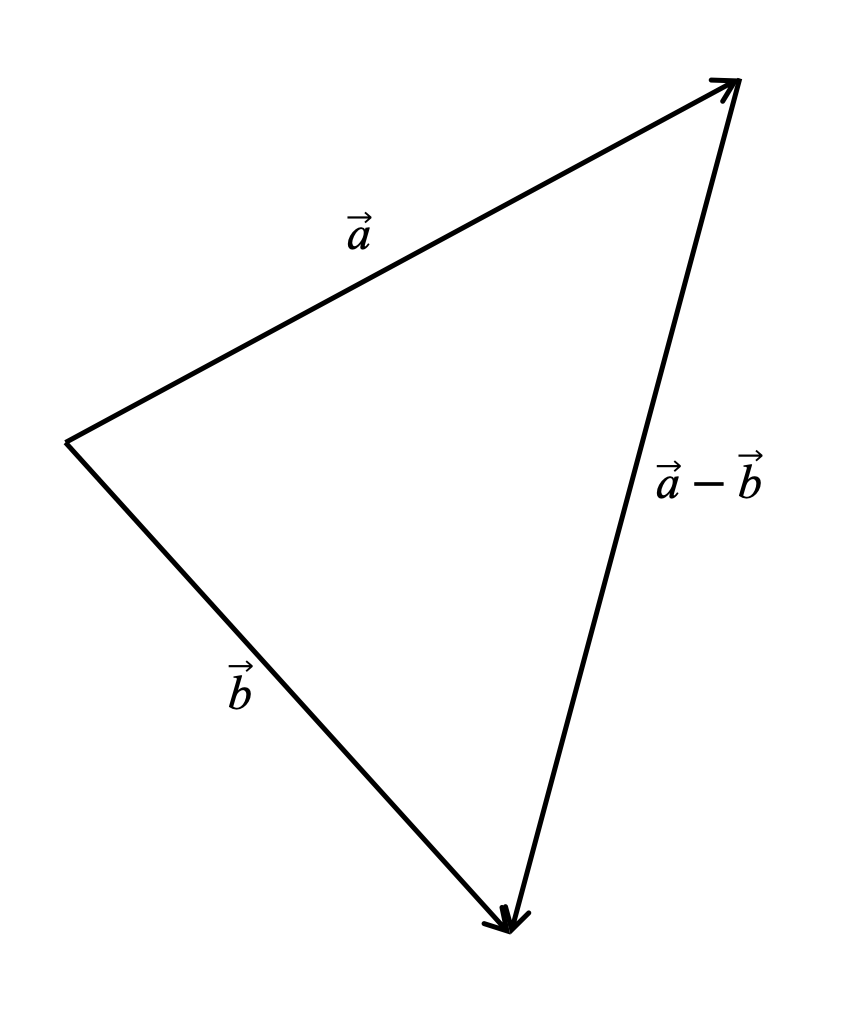
\includegraphics[width=0.5\textwidth]{Fig.3.7.jpg}
      \end{figure}
      By cosine rule: 
      $$\begin{aligned}
        \left|\vec{b}-\vec{a}\right|^2&=\left|\vec{a}\right|^2+\left|\vec{b}\right|^2-2\left|\vec{a}\right|\left|\vec{b}\right|\cos\theta\\
        \left|\vec{b}\right|^2-2\vec{a}\vec{b}+\left|\vec{a}\right|^2&=\left|\vec{a}\right|^2+\left|\vec{b}\right|^2-2\left|\vec{a}\right|\left|\vec{b}\right|\cos\theta\\
        \therefore \vec{a}\cdot\vec{b}&=\left|\vec{a}\right|\left|\vec{b}\right|\cos\theta.
      \end{aligned}$$
    \end{proof}
    \item Combining the two definitions: 
    $${\color{red}{\cos\theta=\frac{a_1b_1+a_2b_2}{\sqrt{\left(a_1^2+a_2^2\right)\left(b_1^2+b_2^2\right)}}}}.$$
  \end{itemize}
  \item 3-D vectors: $\vec{a}=\begin{pmatrix}a_1\\a_2\\a_3\end{pmatrix}$ and $\vec{b}=\begin{pmatrix}b_1\\b_2\\b_3\end{pmatrix}$: 
  \begin{itemize}
    \item $${\color{red}{\vec{a}\cdot\vec{b}=a_1b_1+a_2b_2+a_3b_3}}.$$
    \item $${\color{red}{\cos\theta=\frac{a_1b_1+a_2b_2+a_3b_3}{\sqrt{\left(a_1^2+a_2^2+a_3^2\right)\left(b_1^2+b_2^2+b_3^2\right)}}}}.$$
  \end{itemize}
  \item Properties of scalar product: 
  \begin{itemize}
    \item If ${\color{red}{\vec{a}\cdot\vec{b}=0}}\ \Rightarrow\ {\color{red}{}\begin{cases}\vec{a}=0\\\vec{b}=0\\\vec{a}\text{ and }\vec{b}\text{ are perpendicular (orthogonal)}\ \Rightarrow\ \theta=\frac{\pi}{2}\end{cases}}.$
    \item If $\vec{a}$ and $\vec{b}$ are colinear, $${\color{red}{\vec{a}\cdot\vec{b}=\pm\left|\vec{a}\right|\left|\vec{b}\right|}}.$$
    \begin{proof}
      Angel between $\vec{a}$ and $\vec{b}$ is $0^\circ$.\\
      $\cos0^\circ=1\ \Rightarrow\ \vec{a}\cdot\vec{b}=\left|\vec{a}\right|\left|\vec{b}\right|$ for $\vec{a},\ \vec{b}$ at the same direction.\\
      OR $\vec{a}\cdot\vec{b}=-\left|\vec{a}\right|\left|\vec{b}\right|$ for $\vec{a}$ and $\vec{b}$ at opposite directions. 
    \end{proof}
    \item $${\color{red}{\vec{a}\cdot\vec{b}=\vec{b}\cdot\vec{a}}}.$$
    \item $${\color{red}{\vec{a}\cdot\vec{a}=\left|\vec{a}\right|^2}}$$
    \begin{proof}
      $$\vec{a}\cdot\vec{a}=\begin{pmatrix}a_1\\a_2\end{pmatrix}\begin{pmatrix}a_1\\b_1\end{pmatrix}=a_1^2+a_2^2=\left|\vec{a}\right|^2.$$
    \end{proof}
    \item $${\color{red}{\vec{a}\cdot\left(\vec{b}+\vec{c}\right)=\vec{a}\cdot\vec{b}+\vec{a}\cdot\vec{c}}}.$$
    \item $${\color{red}{\lambda\left(\vec{a}\cdot\vec{b}\right)=\left(\lambda\vec{a}\right)\cdot\vec{b}=\vec{a}\cdot\left(\lambda\vec{b}\right)}}.$$
  \end{itemize}
\end{enumerate}

\subsubsection{Vector Equation of a Line}
\begin{enumerate}
  \item There is only one line that passes through two distinct points. 
  \begin{theorem}
  In the coordinate plane, the equation can be found as: \\
  For $A(x_1,y_1)$ and $B(x_2,y_2)$, the line passes through $A$, $B$ is given by $${\color{red}{y=\frac{y_2-y_1}{x_2-x_1}(x-x_1)+y_1}}.$$
  \end{theorem}
  \item {\color{red}{\textbf{Slope, }$y$\textbf{-intercept form}}}: $y=mx+k$, where $m$ is the slope, and $k$ is the $y$-intercept.\\
  {\color{green}{It can be rearranged to $ax+by=c;\ a,b,c\in\mathbb{R}$, where $a$ and $b$ cannot be equal to $0$ at the same time.}}
  \item \textbf{\color{red}{Vector form}} of a line: 
  \begin{itemize}
    \item For every point $P(x,y)$ that lies on the line $AB$, the vector $\overrightarrow{AP}$ must be collinear or parallel to $\overrightarrow{AB}$: $\overrightarrow{AP}=k\overrightarrow{AB},\ k\in\mathbb{R}$.
    \begin{figure}[H]
      \centering
      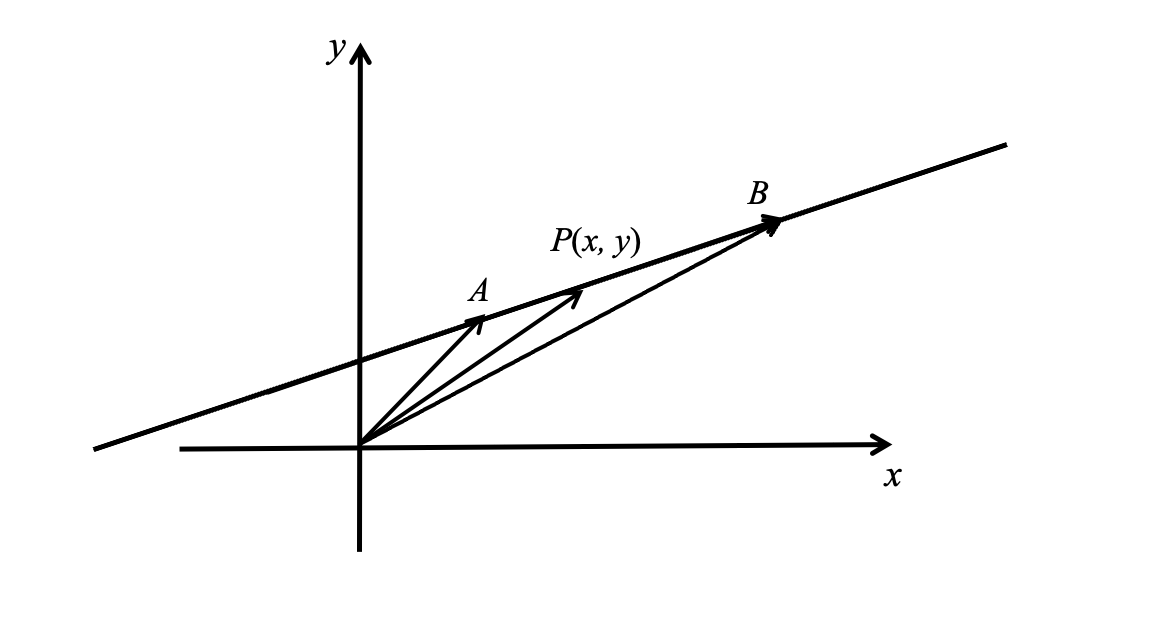
\includegraphics[width=0.5\textwidth]{Fig.3.8.jpg}
    \end{figure}
    \begin{enumerate}
      \item The vector $\overrightarrow{AB}$ is called a \textbf{\color{red}{direction vector}} of the line. \\
      {\color{green}{All the vectors that are parralel to $\overrightarrow{AB}$ can also define the same line.}}
      \item Assume $\overrightarrow{OA}=\vec{a},\ \overrightarrow{OP}=\vec{p},\ \overrightarrow{AB}$ is the direction vector $\vec{d}$. Then, $\overrightarrow{AP}=\vec{p}-\vec{a}=k\overrightarrow{AB}=k\vec{d}$
      $${\color{red}{\vec{p}=\vec{a}+k\vec{d}}},\ k\in\mathbb{R}.$$
    \end{enumerate}
    \item Vector equation of a line: 
    $${\color{red}{\begin{pmatrix}x\\y\end{pmatrix}=\begin{pmatrix}x_1\\y_2\end{pmatrix}+k\begin{pmatrix}d_1\\d_2\end{pmatrix},\ k\in\mathbb{R}}}.$$
    \item Parametric form: 
    $${\color{red}{\begin{cases}x=x_1+kd_1\\y=y_1+kd_2\end{cases},\ k\in\mathbb{R}}}.$$
    \item Cartesian form: 
    $${\color{red}{\frac{x-x_1}{d_1}=\frac{y-y_1}{d_2}}}.$$
    \begin{proof}
      $$\begin{cases}x=x_1+kd_1\\y=y_1+kd_2\end{cases}\Rightarrow\begin{cases}k=\frac{x-x_1}{d_1}\\k=\frac{y-y_1}{d_2}\end{cases}.$$
    \end{proof}
    \begin{enumerate}
      \item Cartesian form can be further rearranged to slope-intercept form
      $$\color{green}
      \begin{aligned}
        \frac{x-x_1}{d_1}&=\frac{y-y_1}{d_2}\\
        \frac{d_2}{d_1}\left(x-x_1\right)&=y-y_1\\
        y&=\frac{d_2}{d_1}\left(x-x_1\right)+y_1,\ 
      \end{aligned}$$
      {\color{green}{where $\frac{d_2}{d_1}$ is the slope. }}
      \item Another way of interpretation: 
      $$\color{green}
      \begin{aligned}
        \overrightarrow{AP}=k\overrightarrow{AB}&\Rightarrow\vec{p}-\vec{a}=k\left(\vec{b}-\vec{a}\right)\\
        &\ \ \ \ \ \ \vec{p}=\left(1-k\right)\vec{a}+k\vec{b},\ k\in\mathbb{R}.\\
        &\Rightarrow \begin{pmatrix}x\\y\end{pmatrix}=\left(1-k\right)\begin{pmatrix}x_1\\y_1\end{pmatrix}+k\begin{pmatrix}x_2\\y_2\end{pmatrix},\ k\in\mathbb{R}.\\
        &\Rightarrow \begin{cases}x=(1-k)x_1+kx_2=x_1+k(x_2-x_1)\\y=(1-k)y_1+ky_2=y_1+k(y_2-y_1)\end{cases},\ k\in\mathbb{R}.\\
        &\Rightarrow \begin{cases}k=\frac{x-x_1}{x_2-x_1}\\y=y_1+k(y_2-y_1)\end{cases}\\
        &\Rightarrow\ y=y_1+\frac{x-x_1}{x_2-x_1}(y_2-y_1)\\
        &\ \ \ \ \ \ \ \ \ =\frac{y_2-y_1}{x_2-x_1}(x-x_1)+y_1.
      \end{aligned}$$
    \end{enumerate}
  \end{itemize}
  \item Orthogonal / Perpendicular vector of a line. 
  \begin{itemize}
    \item There is one and only one line in the plane that is perpendicular to a given line at a particular point on that line. 
    \item Normal Vector: 
    \begin{definition}
      \begin{figure}[H]
        \centering
        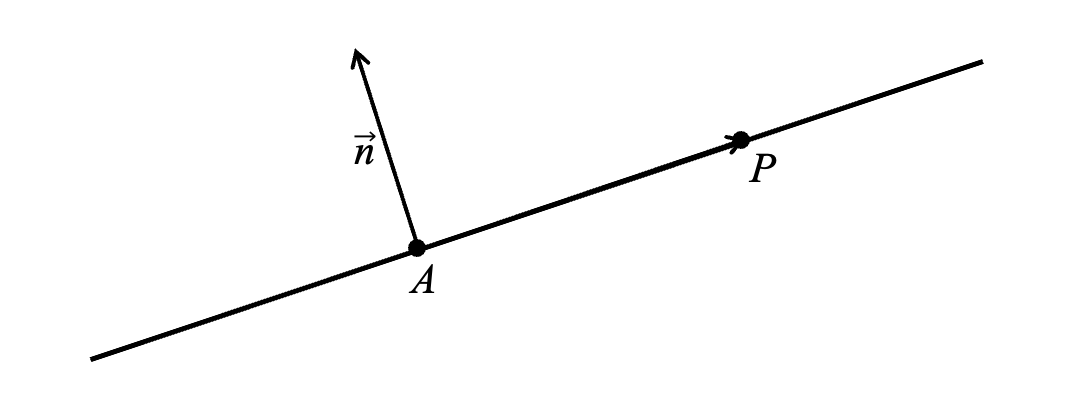
\includegraphics[width=0.5\textwidth]{Fig.3.9.jpg}
      \end{figure}
      A \textbf{\color{red}{normal vector}} is perpendicular or \textbf{orthogonal} to any vector on the lines. 
      $$\text{i.e., }{\color{red}{\vec{n}\cdot}\overrightarrow{AP}=0}.$$
    \end{definition}
    \begin{theorem}
    $$\vec{n}\cdot\left(\vec{p}-\vec{a}\right)=0\ \Rightarrow\ \vec{n}\cdot\vec{p}=\vec{n}\cdot\vec{a}.$$
    \end{theorem}
    \item If the direction vector $\vec{d}=\begin{pmatrix}d_1\\d_2\end{pmatrix}$, then one possible normal vector would be ${\color{red}{\vec{n}=\begin{pmatrix}d_2\\-d_1\end{pmatrix}}}$ or any other vectors parallel to it. 
    \item The vector form: 
    $$\begin{aligned}
      \color{red} \begin{pmatrix}x\\y\end{pmatrix}\cdot\begin{pmatrix}d_2\\-d_1\end{pmatrix}&\color{red}=\begin{pmatrix}x_1\\y_1\end{pmatrix}\cdot\begin{pmatrix}d_2\\-d_1\end{pmatrix}\\
      \color{green} \Rightarrow xd_2-yd_1&\color{green}=x_1d_2-y_1d_1\\
      \color{green}(x-x_1)d_2&\color{green}=yd_1-y_1d_1\\
      \color{red}\therefore y&\color{red}=\frac{d_2}{d_1}(x-x_1)+y_1.
    \end{aligned}$$
  \end{itemize}
  \item Direction vectors: 
  \begin{itemize}
    \item \textbf{\color{red}{Parallel lines}} have \textbf{\color{red}{collinear}} direction vectors. 
    \item \textbf{\color{red}{Perpendicular lines}} have \textbf{\color{red}{orthogonal}} direction vectors, such that the scalar product is equal to 0. 
  \end{itemize}
  \item Vector equation of lines in 3-D spaces: 
  \begin{itemize}
    \item $${\color{red}{\vec{r}=\vec{a}+\lambda\vec{d},\ \lambda\in\mathbb{R}}}.$$
    $${\color{red}{\begin{pmatrix}x\\y\\z\end{pmatrix}=\begin{pmatrix}a_1\\a_2\\a_3\end{pmatrix}+\lambda\begin{pmatrix}d_1\\d_2\\d_3\end{pmatrix}}}.$$
    \item The parametric form: 
    $${\color{red}{\begin{cases}x=a_1+\lambda d_1\\y=a_2+\lambda d_2\\z=a_3+\lambda d_3\end{cases},\ \lambda\in\mathbb{R}}}.$$
    \item The cartesian form: 
    $${\color{red}{\frac{x-a_1}{d_1}=\frac{y-a_2}{d_2}=\frac{z-a_3}{d_3}}}.$$
  \end{itemize}
  \item Two lines: 
  \begin{itemize}
    \item 2-D spaces: two distinctive lines can either be parallel or they can intersect. 
    \item 3-D spaces: 
    \begin{enumerate}
      \item Lines are parallel.
      \item Lines intersect at one common points.
      \item Lines are \textbf{\color{red}{skewed}} (do not intersect and they are not parallel).
    \end{enumerate}
  \end{itemize}
\end{enumerate}

\subsubsection{Vector Product and Properties}
\begin{enumerate}
  \item The vector product is an operation that takes two vectors and results in another {\color{red}{vector}}. 
  \begin{itemize}
    \item Definition
    \begin{definition}
    Given the two vectors and their components, $\vec{a}=\begin{pmatrix}a_1\\a_2\\a_3\end{pmatrix},\ \vec{b}=\begin{pmatrix}b_1\\b_2\\b_3\end{pmatrix},$ then the \textbf{\color{red}{vector product}} is given by: 
    $${\color{red}{\vec{a}\times\vec{b}=\begin{pmatrix}a_2b_3-a_3b_2\\a_3b_1-a_1b_3\\a_1b_2-a_2b_1\end{pmatrix}}}.$$
    \end{definition}
    \item The vector product of two vectors is another vector that is perpendicular to both vectors. 
    \item Magnitude of the vector product: 
    \begin{theorem}
      The magnitude of the vector product is given by the formula $${\color{red}{\left|\vec{a}\times\vec{b}\right|=\left|\vec{a}\right|\cdot\left|\vec{b}\right|\cdot\sin\theta}},$$
      where $\theta$ is the angle between those two vectors. 
      {\color{green}{If $\vec{a}\times\vec{b}=0$, then $\vec{a}$ and $\vec{b}$ are parallel/colinear.}}
    \end{theorem} 
    \item The geometrical definition of cross product (vector product): 
    \begin{theorem}
      Given two vectors $\vec{a}$ and $\vec{b}$, then the vector product is given by $${\color{red}{\vec{a}\times\vec{b}=\left(\left|\vec{a}\right|\left|\vec{b}\right|\sin\theta\right)\widehat{n}}},$$
      where $\widehat{n}$ is the unit vector whose direction is given by the right-hand screw rule to both $\vec{a}$ and $\vec{b}$ and the vectors $\vec{a},\ \vec{b},$ and $\widehat{n}$ follows the right-hand rule. 
    \end{theorem}
    \item Geometrical meaning of the magnitude of the vector product: \\
    It is equal to the area of the parallelogram enclosed by those two vectors. 
  \end{itemize}
  \item Properties of the vector product: 
  \begin{itemize}
    \item $${\color{red}{\vec{a}\times\vec{b}=-\left(\vec{b}\times\vec{a}\right)}}$$
    \item $${\color{red}{\left(\vec{a}\times\vec{b}\right)\times\vec{c}=\vec{a}\times\left(\vec{b}\times\vec{c}\right)}}$$
    \item $${\color{red}{\lambda\left(\vec{a}\times\vec{b}\right)=\left(\lambda\vec{a}\right)\times\vec{b}=\vec{a}\times\left(\lambda\vec{b}\right),\ \lambda\in\mathbb{R}}}$$
    \item $${\color{red}{\left(\vec{a}+\vec{b}\right)\times\vec{c}=\left(\vec{a}\times\vec{c}\right)+\left(\vec{b}\times\vec{c}\right)}}.$$
  \end{itemize}
  \item Mixed product: 
  \begin{itemize}
    \item An operation with three vectors $\vec{a},\ \vec{b},$ and $\vec{c}$ combining both the vector and scalar product is called a \textbf{\color{red}{mixed product}}: 
    $${\color{red}{\left(\vec{a}\times\vec{b}\right)\cdot\vec{c}}}.$$
    \item Given $\vec{a}=\begin{pmatrix}a_1\\a_2\\a_3\end{pmatrix},\ \vec{b}=\begin{pmatrix}b_1\\b_2\\b_3\end{pmatrix},$ and $\vec{c}=\begin{pmatrix}c_1\\c_2\\c_3\end{pmatrix}$, the mixed product is given by: 
    $$\color{red}
    \begin{aligned}
      \left(\vec{a}\times\vec{b}\right)\cdot\vec{c}&=\begin{pmatrix}a_2b_3-a_3b_2\\a_3b_1-a_1b_3\\a_1b_2-a_2b_1\end{pmatrix}\cdot\begin{pmatrix}c_1\\c_2\\c_3\end{pmatrix}\\
      &=a_1b_2c_3+a_2b_3c_1+a_3b_1c_2-a_1b_3c_2-a_2b_1c_3-a_3b_2c_1
    \end{aligned}$$
    \item Geometric meaning of mixed products: \\
    The volume of a parallelepiped fromed by three non-coplanar vectors, $\vec{a}$, $\vec{b}$, and $\vec{c}$ is given by: 
    $${\color{red}{V=\left|\left(\vec{a}\times\vec{b}\right)\cdot\vec{c}\right|}}.$$
    \begin{proof}
      \begin{figure}[H]
        \centering
        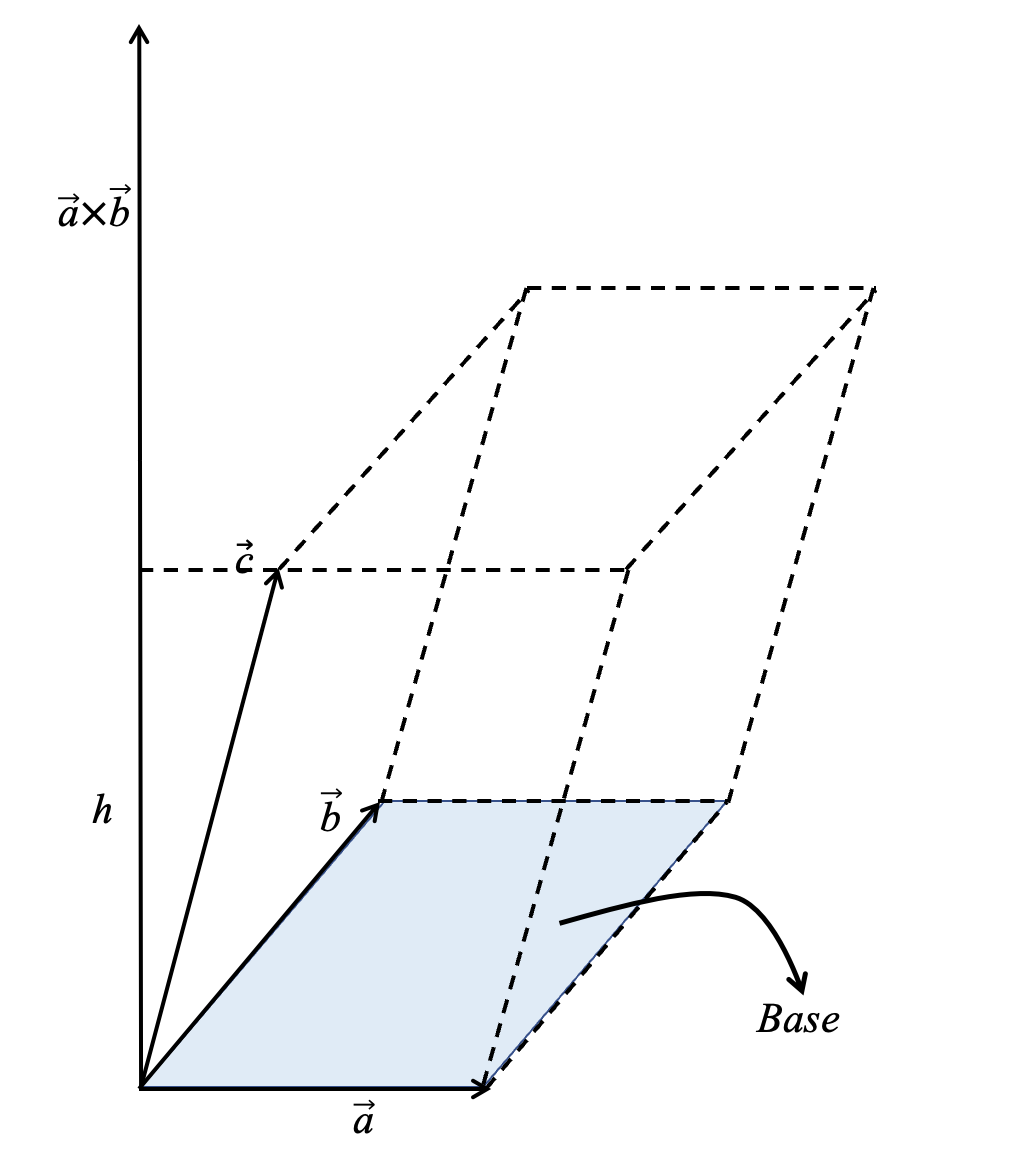
\includegraphics[width=0.3\textwidth]{Fig.3.10.jpg}
      \end{figure}
      $$V=\text{Base}\times h$$
      Base=magnitude of cross product of $\vec{a}$ and $\vec{b}$.\\
      $=$ perpendicular projection of $\vec{c}$ to $\vec{a}\times\vec{b}$.\\
      $$\therefore V=\text{Base}\times h=\left|\vec{a}\times\vec{b}\right|\cdot\left|\vec{c}\right|\cdot\left|\cos\theta\right|=\left|\left(\vec{a}\times\vec{b}\right)\cdot\vec{c}\right|$$
    \end{proof}
    \item Three or more vectors are said to be coplanar if they lie in the same plane.
    \item Using mixed product to find the volume of a triangular pyramid: 
    $${\color{red}{V=\frac{1}{6}\left|\left(\vec{a}\times\vec{b}\right)\cdot\vec{c}\right|}}.$$
    \begin{proof}
      \begin{figure}[H]
        \centering
        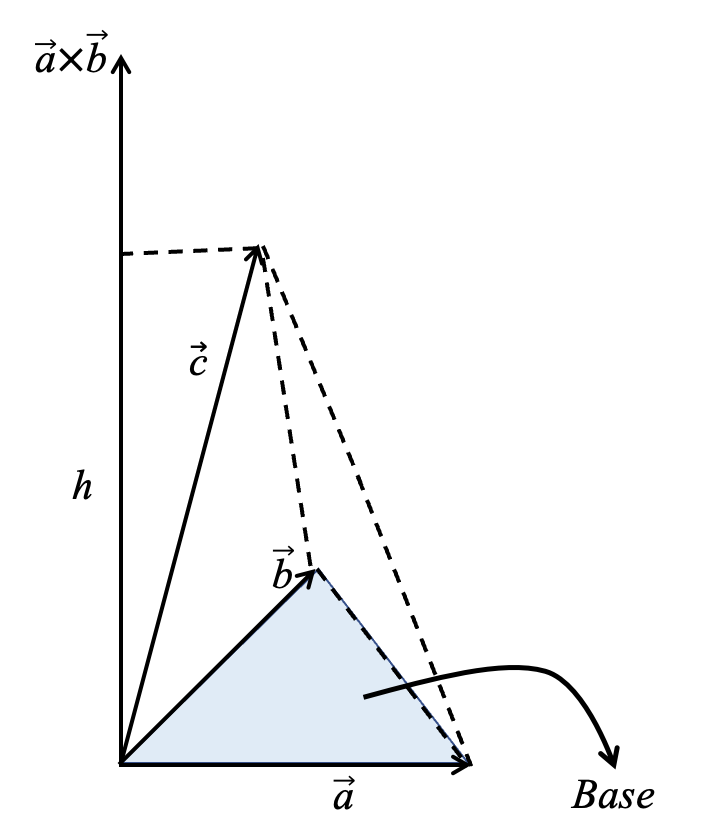
\includegraphics[width=0.3\textwidth]{Fig.3.11.jpg}
      \end{figure}
      Since the base is not a parallelogram but a triangle, that is half an area of the parallelogram, we multiply $\frac{1}{2}$ in front of the expression of the cross product.
      $$\text{Base}=\frac{1}{2}\left|\vec{a}\times\vec{b}\right|.$$
      The volume of a pyramid is $\frac{1}{3}$ of the product of the base and the height. 
      $$\therefore V=\frac{1}{3}\text{Base}\cdot h=\frac{1}{3}\cdot\frac{1}{2}\left|\vec{a}\times\vec{b}\right|\left|\vec{c}\right|\left|\cos\theta\right|=\frac{1}{6}\left|\left(\vec{a}\times\vec{b}\right)\cdot\vec{c}\right|$$ 
    \end{proof}
  \end{itemize}
  \item Proving vector product using matrix. 
  \begin{proof}
    Let $\vec{a}=\begin{pmatrix}a_1\\a_2\\a_3\end{pmatrix},\ \vec{b}=\begin{pmatrix}b_1\\b_2\\b_3\end{pmatrix}$. Convert into a $3\times 3$ matrix: $\begin{bmatrix}\vec{i}&\vec{j}&\vec{k}\\a_1&a_2&a_3\\b_1&b_2&b_3\end{bmatrix}.$\\
    Find the determinant: $\left|\begin{matrix}\vec{i}&\vec{j}&\vec{k}\\a_1&a_2&a_3\\b_1&b_2&b_3\end{matrix}\right|=\vec{i}(a_2b_3-a_3b_2)-\vec{j}(a_1b_3-a_3b_1)+\vec{k}(a_1b_2-a_2b_1)$
    $$\Rightarrow \begin{pmatrix}a_2b_3-a_3b_2\\a_3b_1-a_1b_3\\a_1b_2-a_2b_1\end{pmatrix}.$$
  \end{proof}
\end{enumerate}

\subsubsection{Vector Equation of a Plane}
\begin{enumerate}
  \item A plane is uniquely determined by {\color{red}{three points}} (or a line and a point outside the line).\\
  $\rightarrow$ A plane can also be determined by two intersecting lines and a point outside the lines. 
  \item Vector equation of a plane: 
  $${\color{red}{\vec{r}=\vec{a}+\lambda\vec{d_1}+\mu\vec{d_2},\ \lambda,\mu\in\mathbb{R}}}.$$
  where $\vec{d_1}$ and $\vec{d_2}$ are direction vectors, and $\vec{a}$ is the position vector. 
  \begin{figure}[H]
    \centering
    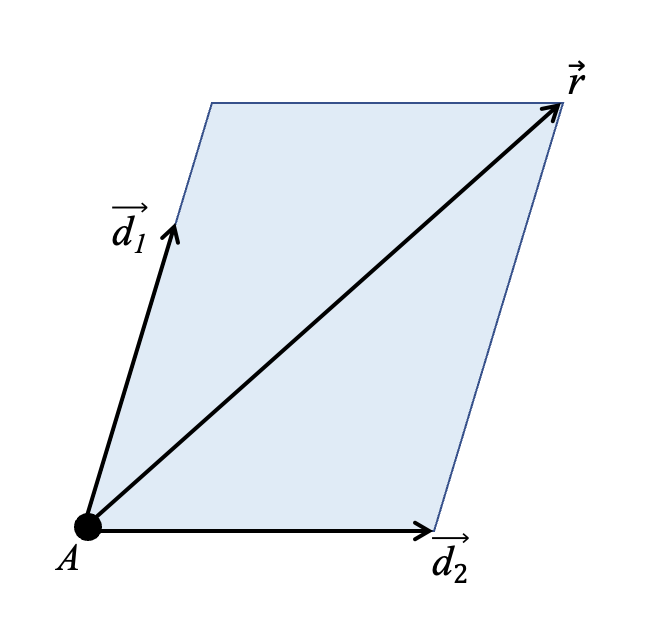
\includegraphics[width=0.3\textwidth]{Fig.3.12.jpg}
  \end{figure}
  \item The scalar product form: 
  \begin{itemize}
    \item \textbf{\color{red}{Normal vector}} is a vector that is perpendicular to every line in the plane. 
    \begin{figure}[H]
      \centering
      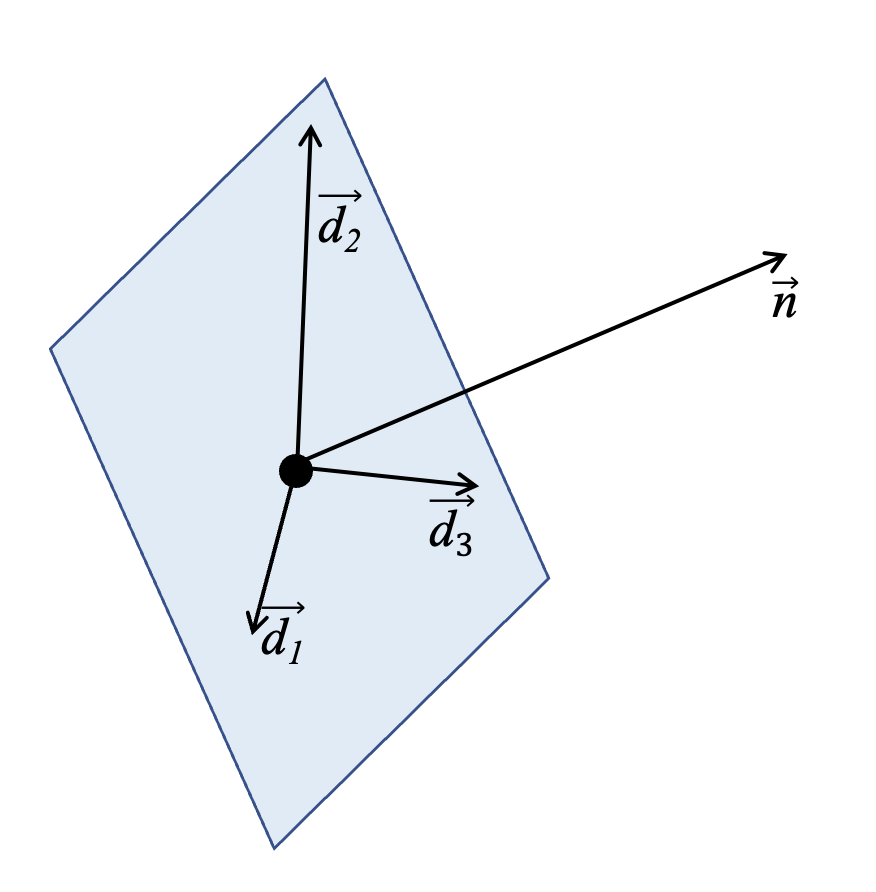
\includegraphics[width=0.3\textwidth]{Fig.3.13.jpg}
    \end{figure}
    \item All planes with the same normal vector are parallel to each other. 
    \item If $R$ is any other point on the plane, then $\overrightarrow{AR}$ lies in the plane, and it is perpendicular to the normal vector $\vec{n}$.
    \begin{theorem}
      $$\color{red} \overrightarrow{AR}\cdot\vec{n}=0\ \Rightarrow\ \left(\vec{r}-\vec{a}\right)\cdot\vec{n}=0$$
      $$\color{red} \therefore \vec{r}\cdot\vec{n}=\vec{a}\cdot\vec{n}$$
      where $\vec{a}$ is the position vector, and $\vec{n}$ is the normal vector. 
    \end{theorem}
  \end{itemize}
  \item The Cartesian equation of a plane: 
  $${\color{red}n_1x+n_2y+n_3z=d},\ \text{where }n=\begin{pmatrix}n_1\\n_2\\n_3\end{pmatrix},\ d=\vec{a}\cdot\vec{n}.$$
  \begin{proof}
    $$\vec{n}=\begin{pmatrix}n_1\\n_2\\n_3\end{pmatrix},\ d=\vec{a}\cdot\vec{n},\ \vec{r}=\begin{pmatrix}x\\y\\z\end{pmatrix}$$
    The scalar product form converts to: 
    $$\begin{pmatrix}x\\y\\z\end{pmatrix}\cdot\begin{pmatrix}n_1\\n_2\\n_3\end{pmatrix}=\vec{a}\cdot\vec{n}$$
    $$\Rightarrow n_1x+n_2y+n_3z=d.$$
  \end{proof}
  \item A plane with the vector equation $\vec{r}=\vec{a}+\lambda\vec{d_1}+\mu\vec{d_2}$ has a normal vector ${\color{red}{\vec{n}=\vec{d_1}\times\vec{d_2}}}.$
\end{enumerate}

\subsubsection{Lines, Planes, and Angles}
\begin{enumerate}
  \item Angles and intersections between lines and planes: 
  \begin{itemize}
    \item When a line intersects a plane, the angle between them is defined as the {\color{red}{smallest possible angle}} that the line makes with any of the lines in the plane. 
    \begin{figure}[H]
      \centering
      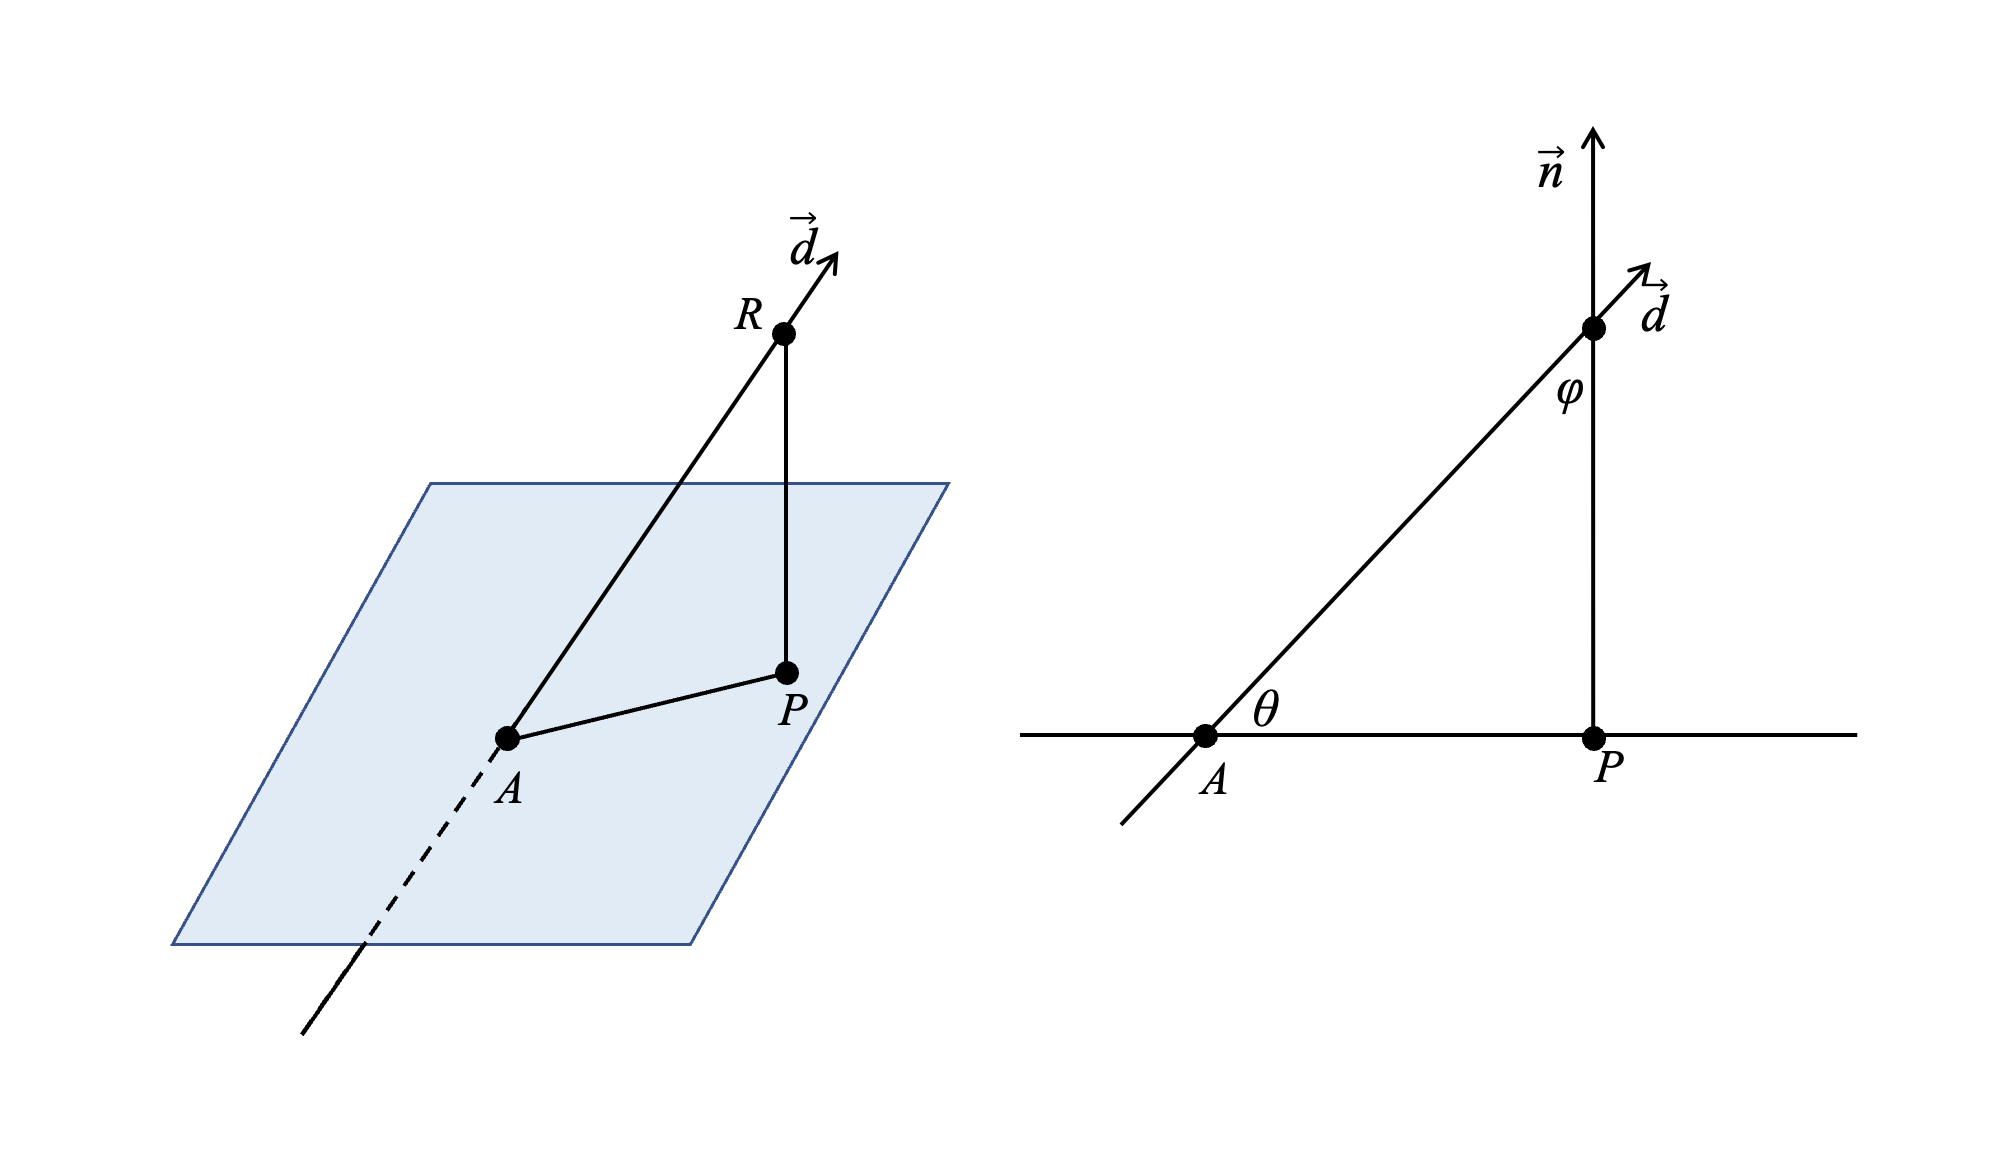
\includegraphics[width=0.8\textwidth]{Fig.3.14.jpg}
    \end{figure}
    \begin{enumerate}
      \item $\overrightarrow{AR}$: the direction vector of the line, $\vec{d}$.
      \item Point $P$ is the projection of point $R$ onto the plane. $\overrightarrow{AP}$ is the shadow of $\overrightarrow{AR}$ on the plane. 
      \item $\overrightarrow{PR}$ is in the direction of $\vec{n}$ since it is perpendicular to the plane. 
      \item $\varphi$ is the angle between $\vec{n}$ and $\vec{d}$. 
      \item $$\color{red} \theta=90^\circ-\varphi,\ \cos\varphi=\frac{\left|\vec{n}\cdot\vec{d}\right|}{\left|\vec{n}\right|\left|\vec{d}\right|}.$$
    \end{enumerate}
    \item A line that is not parallel to a plane intersects a plane at one point. The coordinates of this point of intersection satisfies both the equation of the line and the equation of the plane. 
  \end{itemize}
  \item Relationship of two planes: 
  \begin{itemize}
    \item Two planes can either intersect at a line or they can be parallel.
    \item When two planes are parallel, their normal vectors are {\color{red}{colinear}}; otherwise they intersect at a line. 
  \end{itemize}
  \item Angles between two planes: 
  \begin{itemize}
    \item The angle between two planes is \textbf{\color{red}{the angle between their normal vectors}}.
    \item $$\color{red} \cos\theta=\frac{\vec{n_1}\cdot\vec{n_2}}{\left|\vec{n_1}\right|\left|\vec{n_2}\right|}.$$
    \begin{figure}[H]
      \centering
      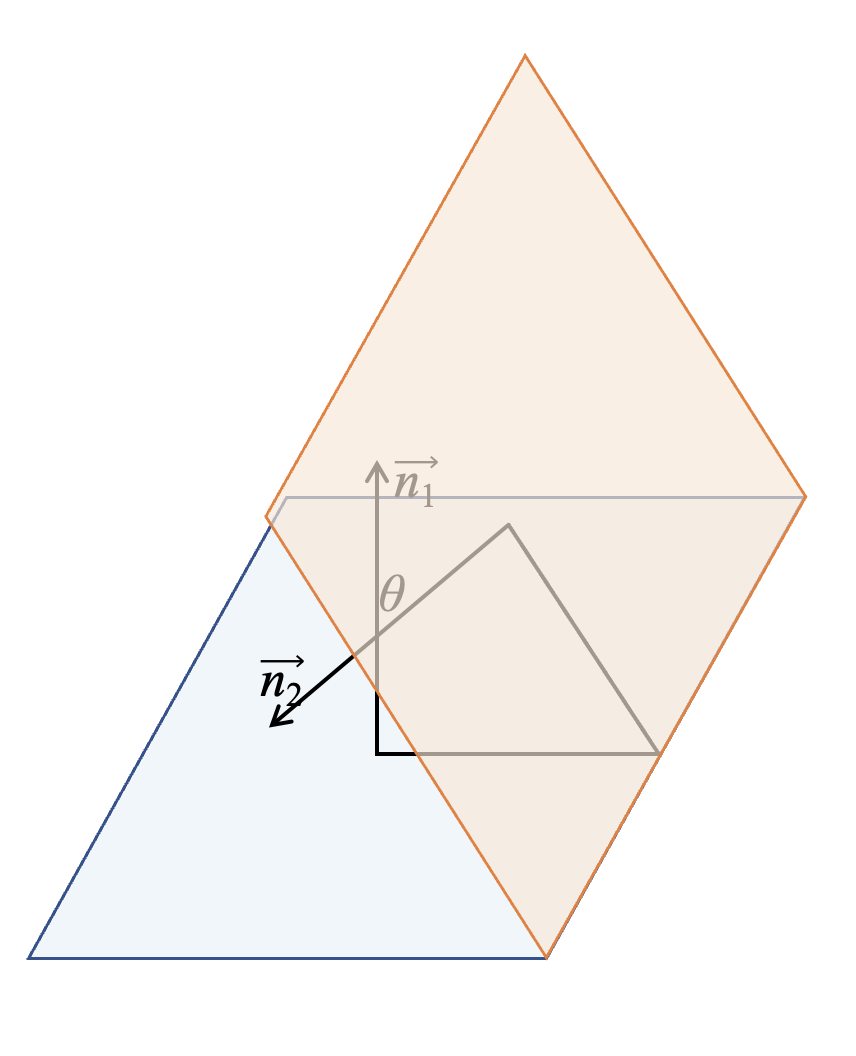
\includegraphics[width=0.5\textwidth]{Fig.3.15.jpg}
    \end{figure}
  \end{itemize}
  \item Two non-parallel planes intersect along a line. The equation of this line is formed by treating the Cartesian equation of two planes as simultaneous equations and finding the general solution.
  \item Distance between a point and a plane. 
  \begin{itemize}
    \item The distance, $d$, between a point $P(x_0,y_0,z_0)$, and a plane with equation $Ax+By+Cz=D$ where $\vec{n}=A\vec{i}+B\vec{j}+C\vec{k}$, is given by: 
    $${\color{red}{d=\frac{\left|Ax_0+By_0+Cz_0-D\right|}{\sqrt{A^2+B^2+C^2}}}}.$$ 
    \item Proof: 
    \begin{proof}
      \begin{figure}[H]
        \centering
        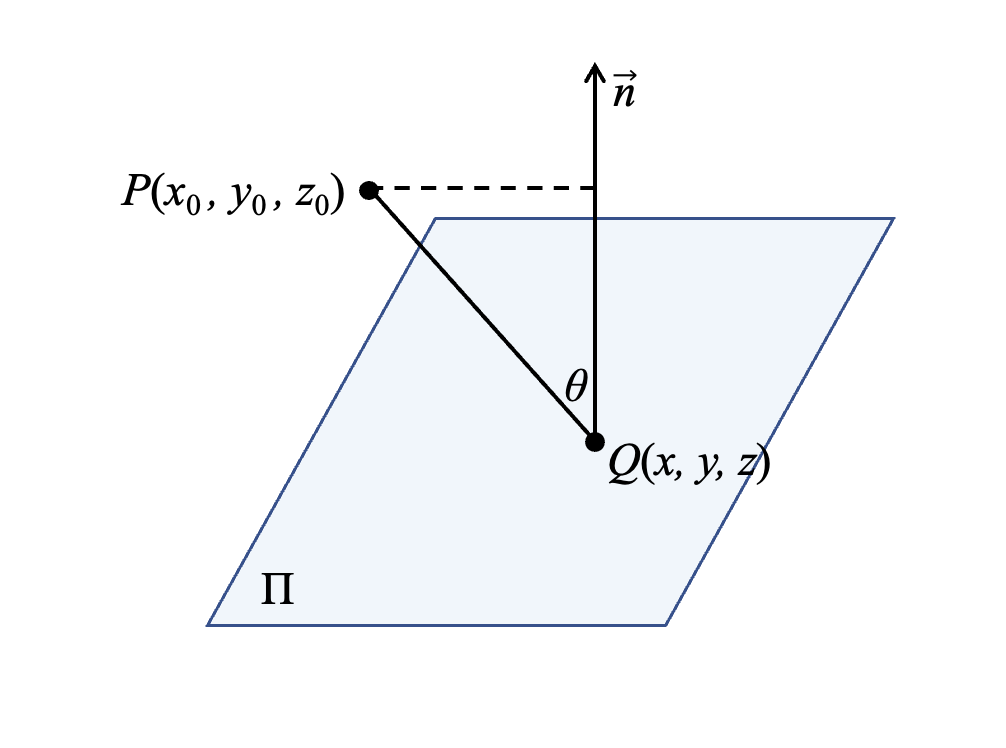
\includegraphics[width=0.5\textwidth]{Fig.3.16.jpg}
      \end{figure}
      Let $Q(x,y,z)$ be any point on the plane $\Pi$.\\
      The distance, $d$, is the projection of the distance of point $P$ to the plane on the normal vector, $\vec{n}$.
      $$\begin{aligned}
        d&=\left|\overrightarrow{QP}\right|\cdot\left|\cos\theta\right|=\left|\overrightarrow{QP}\right|\cdot\frac{\overrightarrow{QP}\cdot\vec{n}}{\left|\overrightarrow{QP}\right|\cdot\left|\vec{n}\right|}\\
        &=\frac{\overrightarrow{QP}\cdot\vec{n}}{\left|\vec{n}\right|}=\frac{\left|\left\langle A,B,C\right\rangle\cdot\left\langle (x_0-x), (y_0-y), (z_0-z)\right\rangle\right|}{\sqrt{A^2+B^2+C^2}}\\
        &=\frac{\left|Ax_0+By_0+Cz_0-(Ax+By+Cz)\right|}{\sqrt{A^2+B^2+C^2}}\\
        &=\frac{Ax_0+Bx_0+Cz_0-D}{\sqrt{A^2+B^2+C^2}}
      \end{aligned}$$
    \end{proof}
  \end{itemize}
  \item Intersection of three points: 
  \begin{itemize}
    \begin{figure}[H]
      \centering
      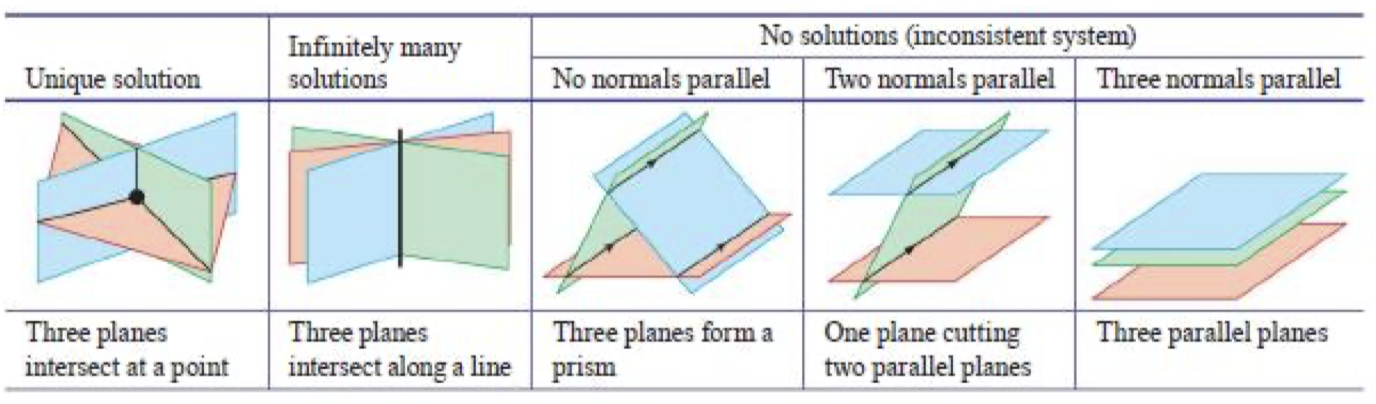
\includegraphics[width=0.9\textwidth]{Fig.3.17.jpg}
    \end{figure}
    \item The plane intersect: 
    \begin{enumerate}
      \item At a point: {\color{green}{the system of equations will have a unique solution.}}
      \item Alone a line: {\color{green}{the system of equations will have infinitely many solutions}}
    \end{enumerate}
    \item The systems of equations have no solutions: 
    \begin{enumerate}
      \item No normals are parallel {\color{green}{(the planes from a prism)}}
      \item 2 normals are parallel or three normal are parallel {\color{green}{(the planes are parallel)}}
    \end{enumerate}
  \end{itemize}
\end{enumerate}

\newpage
\section{Topic 4 Statistics}
\begin{center}
\textbf{\textit{Content Pending}}
\end{center}

\newpage
\section{Topic 5 Calculus}
\subsection{Limits}
\begin{enumerate}
    \item Limit
    \begin{example}
        $$\lim_{x\rightarrow 1}\frac{x^2-1}{x-1}=2$$
        when $x$ is {\color{red}{approaching to}} $1$ (it never equals to $1$), the value $\frac{x^2-1}{x-1}$ is appraoching to 2.
    \end{example}
    \begin{itemize}
        \item Left-hand and Right-hand Limit 
        \begin{figure}[H]
            \centering 
            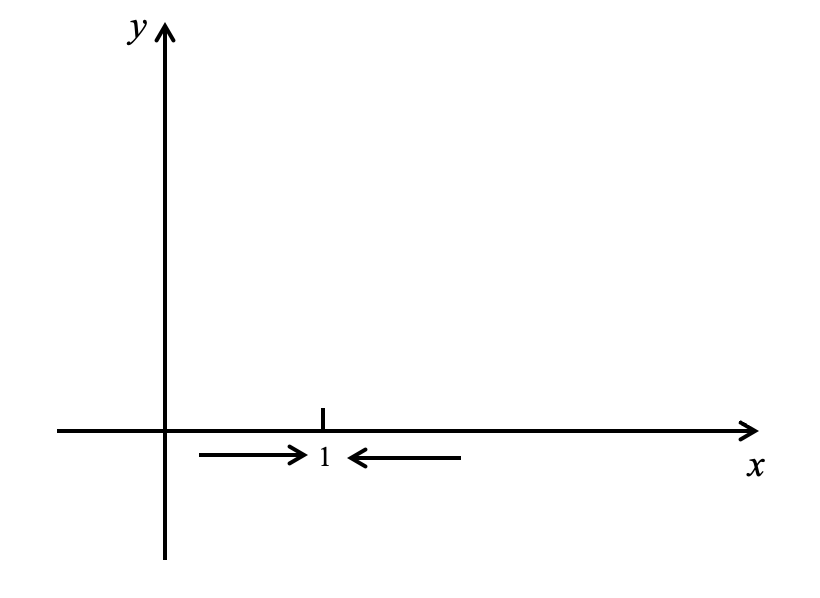
\includegraphics[width=0.5\textwidth]{Fig.5.1.jpg} 
        \end{figure}
        \begin{example}
            The left-hand limit of $\frac{x^2-1}{x-1}$ when $x \rightarrow 1$ is $$\lim_{x \rightarrow 1^-}\frac{x^2-1}{x-1}=2.$$
            The right-hand limit of $\frac{x^2-1}{x-1}$ when $x \rightarrow 1$ is $$\lim_{x \rightarrow 1^+}\frac{x^2-1}{x-1}=2.$$
        \end{example}
        \item Only when the left-hand limit and the right-hand limit exist and are the same at the point $x=a$, we say the limit of $f(x)$ exists on $x=a$. 
        $$\text{i.e., }{\color{red}{\lim_{x\rightarrow a^-}f(x)=\lim_{x\rightarrow a^+}f(x)=c\ \Rightarrow\ \lim_{x\rightarrow a}f(x)=c}},\ c\text{ is a constant}\in \mathbb{R}$$
        Otherwise, the limit does not exist on $x=a$ {\color{green}(OR DNE.)}.
        \begin{example}
            \textbf{Does $\lim\limits_{x\rightarrow 0}\frac{1}{x}$ exist? How about $\lim\limits_{x\rightarrow \infty}\frac{1}{x}$?}
            \begin{figure}[H]
                \centering 
                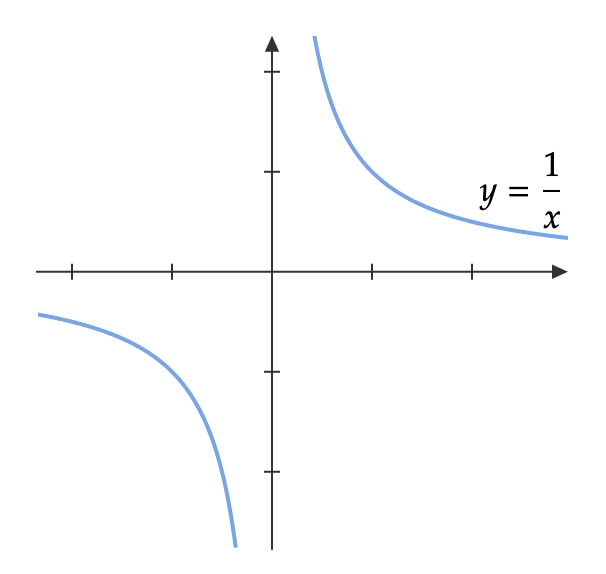
\includegraphics[width=0.5\textwidth]{Fig.5.2.jpg} 
            \end{figure}
            \begin{itemize}
                \item $\lim\limits_{x\rightarrow 0}\frac{1}{x}$ doest not exist. 
                $$\because \lim_{x\rightarrow 0^+}\frac{1}{x}=+\infty,\ \lim_{x\rightarrow 0^-}\frac{1}{x}=-\infty$$
                $$\therefore \lim_{x\rightarrow 0^+}\frac{1}{x}\neq\lim_{x\rightarrow 0^-}\frac{1}{x} \Rightarrow \text{DNE.} $$
                \item $\lim\limits_{x\rightarrow \infty}\frac{1}{x}$ exists. 
                $$\because \lim_{x\rightarrow +\infty}\frac{1}{x}=0,\ \lim_{x\rightarrow -\infty}\frac{1}{x}=0$$
                $$\therefore \lim_{x\rightarrow +\infty}\frac{1}{x}=\lim_{x\rightarrow -\infty}\frac{1}{x} \Rightarrow \text{Limit exists.}$$
            \end{itemize}
        \end{example}
        \begin{definition}
            {\color{red}\textbf{Horizontal Asymptote (H.A.)}}: 
            $$y=\lim_{x\rightarrow \infty}f(x)=c$$
        \end{definition}
        \item Limit at $\infty$: 
        $${\color{red}\lim_{x\rightarrow +\infty}f(x)=\lim_{x\rightarrow -\infty}f(x)=c\ \Rightarrow \ \lim_{x\rightarrow \infty}f(x)=c}.$$
        {\color{green}{Note: $+\infty$ and $-\infty$ are not exact values; they should be regarded as a concept.}}
        \item Limites does not have to equal to the function value. \\
        Limit and the function value do not have relationships.
        \item Generally speaking, if $a \in D_f,\ \lim\limits_{x\rightarrow a}f(x)=f(a)$.
    \end{itemize}
    \item For a rational function $f(x)=\frac{P(x)}{Q(x)}$ where $P(x)=a_0x^m+a_1x^{m-1}+\cdots+a_{m-1}x+a_m$, and $Q(x)=b_0x^m+b_1x^{m-1}+\cdots+b_{m-1}x+b_m$:
    \begin{itemize}
        \item $\lim\limits_{x\rightarrow a}f(x)=f(a)\text{ as long as }Q(a)\neq 0.$
        \item $\lim\limits_{x\rightarrow \infty}f(x)=\lim\limits_{x\rightarrow \infty}\frac{a_0x^m+a_1x^{m-1}+\cdots+a_{m-1}x+a_m}{b_0x^m+b_1x^{m-1}+\cdots+b_{m-1}x+b_m}\ \Rightarrow\ \text{H.A.}$
        \begin{enumerate}
            \item If $m=n$, $\lim\limits_{x\rightarrow \infty}f(x)=\lim\limits_{x\rightarrow \infty}\frac{a_0}{b_0}=\frac{a_0}{b_0}.$
            \item If $m>n$, $\lim\limits_{x\rightarrow \infty}f(x)\text{ DNE.}$
            \item If $m<n$, $\lim\limits_{x\rightarrow \infty}f(x)=0.$
        \end{enumerate}
    \end{itemize}
    \item Continuity and Discontinuity
    \begin{definition}
        {\color{red}\textbf{Continuity}}: If the graph of the function does not have any {\color{red}{breaks or holes}} within a certain interval, then the function is continuous within that interval.
    \end{definition}
    \begin{theorem}
        If ${\color{red}{\lim\limits_{x\rightarrow a^-}f(x)=\lim\limits_{x\rightarrow a^+}f(x)=f(a)}}$, then the function $f$ is \textbf{continuous} at $x=a$.
    \end{theorem}
\end{enumerate}

\subsection{Differentiation and Derivatives}
\begin{enumerate}
    \item Gradient of Secant: 
    \begin{figure}[H]
        \centering 
        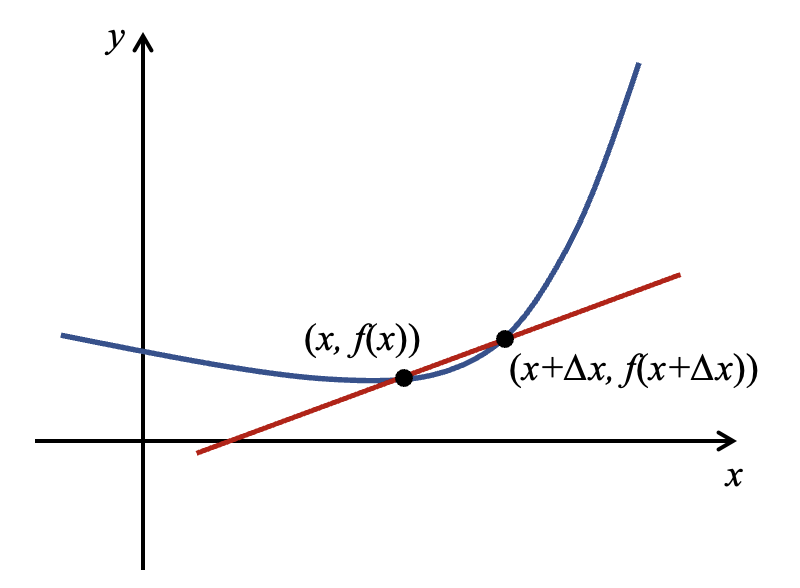
\includegraphics[width=0.5\textwidth]{Fig.5.3.jpg} 
    \end{figure}
    \begin{itemize}
        \item $$\text{Slope }m=\frac{f(x+\Delta x)-f(x)}{x+\Delta x-x}=\frac{f(x+\Delta x)-f(x)}{\Delta x}.$$
        \begin{definition}
            \textbf{\color{red}Derivative of a function}: 
            $${\color{red}\lim_{\Delta x\rightarrow 0}\frac{f(x+\Delta x)-f(x)}{\Delta x}}\text{ is the derivative of a function, denoted as } {\color{red}\frac{\mathrm{d}y}{\mathrm{d}x}}\text{ or }{\color{red}f'(x)}.$$
        \end{definition}
    \item The graphic meaning of derivative is the gradient of tangent of the function. 
    \begin{example}
        \textbf{By definition, find the derivative of $f(x)=x^2+1$ and hance find the gradient of the tangent line when $x=3$.}
        $$\begin{aligned}
            f'(x)=\lim_{x\to 0}\frac{f(x+\Delta x)-f(x)}{\Delta x}&=\lim_{x\to 0}\frac{\left[(x+\Delta x)^2+1\right]-(x^2+1)}{\Delta x}\\
            &=\lim_{x\to 0}\frac{x^2+2x\Delta x+(\Delta x)^2+1-x^2-1}{\Delta x}\\
            &=\lim_{x\to 0}\frac{2x\Delta x+(\Delta x)^2}{\Delta x}\\
            &=\lim_{x\to 0}\left(2x+\Delta x\right)\\
            &=2x.
        \end{aligned}$$
        At $x=3$, $f'(3)=2\times 3=6.$ The gradient is $6.$
    \end{example}
    \end{itemize}
    \item Derivative of $x^n$
    \begin{theorem}
        If $f(x)=x^n$, then 
        $${\color{red}{f'(x)=nx^{n-1}}},\ \text{for any } n \in \mathbb{R}.$$
        Note: The derivative of any {\color{red}{constant}} is {\color{red}{0}}.
    \end{theorem}
    \begin{example}
        $$f(x)=\frac{1}{x}=x^{-1}\ \Rightarrow\ f'(x)=(-1)x^{-1-1}=-x^{-2};$$
        $$f(x)=\sqrt{x}=x^{\frac{1}{2}}\ \Rightarrow\ f'(x)=\frac{1}{2}x^{\frac{1}{2}-1}=\frac{1}{2}x^{-\frac{1}{2}};$$
        $$f(x)=c=cx^0\ \Rightarrow\ f'(x)=0\times cx^{0-1}=0.$$
    \end{example}
    \item Rules of Differentiation: \\
    Name $f(x)$ and $g(x)$ as two functions with derivatives of $f'(x)$ and $g'(x)$, respectively.\\
    Then {\color{red}{$$\left(cf(x)\right)'=cf'(x)$$
    $$\left(f(x)\pm g(x)\right)'=f'(x)\pm g'(x)$$}}
    \item More Derivatives: 
    \begin{center}\begin{tabular}{c|c}
        $f(x)$&$f'(x)$\\ \hline
        $\sin x$&$\cos x$\\ 
        $\cos x$&$-\sin x$\\ 
        $\tan x$&$\sec^2x$\\
        $\ln x$&$\frac{1}{x}$\\
        $e^x$&$e^x$
    \end{tabular}\end{center}
    \item Differentiablity: 
    \begin{definition}
        A function has to be \textbf{continuous} and \textbf{no sharp turning point} to be \textbf{\color{red}{differentiable}}.\\
        {\color{green}{Note: Smooth turning point on the graph is allowed.}}
    \end{definition}
    \item More Rules of Differentiation: 
    \begin{theorem}
        Let $f(x)$ and $g(x)$ be two functions with derivatives of $f'(x)$ and $g'(x)$, respectively.
        \color{red}{$$\left(f(x)\times g(x)\right)'=f'(x)g(x)+f(x)g'(x).$$}
    \end{theorem}
    \begin{theorem}
        Let $f(x)$ and $g(x)$ be two functions with derivatives of $f'(x)$ and $g'(x)$, respectively.
        \color{red}{$$\left(\frac{f(x)}{g(x)}\right)'=\frac{f'(x)g(x)-f(x)g'(x)}{g^2(x)}.$$}
    \end{theorem}
    \begin{theorem}
        For a composite function $f(g(x))$ or $(f\circ g)(x)$, the derivative will be $${\color{red}{f'(g(x))\times g'(x)}}.$$
        OR \\
        If $y=f(u)$ and $u=g(x)$, then $${\color{red}{\frac{\mathrm{d}y}{\mathrm{d}x}=\frac{\mathrm{d}y}{\mathrm{d}u}\cdot\frac{\mathrm{d}u}{\mathrm{d}x}}}.$$
    \end{theorem}
    \item Higher Order Differentiation: 
    $$\frac{\mathrm{d}^2y}{\mathrm{d}x^2},\ f''(x),\ f'''(x),\ f^{(4)}(x),\ f^{(5)}(x),\ \cdots$$
\end{enumerate}

\subsection{Applications of Derivatives}
\begin{enumerate}
    \item Equation of Tangent Line: \\
    Via the original functions, we could get the tangent point $(x_0, y_0)$. Then, the expression of the tangent line is 
    $${\color{red}{y-y_0=m(x-x_0)}},$$ 
    where $m$ is the derivative. 
    \item Normal and Tangent Lines: 
    \begin{definition}
        \textbf{\color{red}{Normal}} is perdendicular to the tangent and passes through the same tangent point. 
        \begin{figure}[H]
            \centering 
            \includegraphics[width=0.5\textwidth]{Fig.5.4.jpg} 
        \end{figure}
    \end{definition}
    \item Increasing and Decreasing Function: 
    \begin{definition}
        \textbf{\color{red}{Increasing Function}}: As $x$ is getting larger, $y$ is getting larger.\\
        i.e., $${\color{red}{\frac{\mathrm{d}y}{\mathrm{d}x}>0}}.$$
        \textbf{\color{red}{Decreasing Function}}: As $x$ is getting larger, $y$ is getting smaller.\\
        i.e., $${\color{red}{\frac{\mathrm{d}y}{\mathrm{d}x}<0}}.$$
    \end{definition}
    \item Local Extrema: $\color{red}{\frac{\mathrm{d}y}{\mathrm{d}x}=0}$ {\color{red}{Stationary point}}\\
    {\color{green}{Global extrema is the maximum and the minimum points of the entire function.}}\\
    $f''(x)$ is used to determine if the local extrema is maxima or minima.
    \begin{itemize}
        \item {\color{red}{Minima: $f''(x)>0$}} Concave up.
        \item {\color{red}{Maxima: $f''(x)<0$}} Concave down.
        \item {\color{red}{Point of Inflection {\color{green}{(the point that is changing from concaving up to concaving down, or vice visa)}}: $f''(x)=0$}}
    \end{itemize}
    \item With local extrema, $x$-intercepts, $y$-intercepts, concavity, and asympotes, draw approxiate diagrams of a function.
\end{enumerate}

\subsection{Implicit Differentiation}
\begin{enumerate}
    \item When differentiating something with $\color{red}{y}$, multiply $\color{red}{\frac{\mathrm{d}y}{\mathrm{d}x}}$ at the end. 
    \item $\color{red}{(y^2)'=2y\frac{\mathrm{d}y}{\mathrm{d}x}}$.
    \begin{proof}
        If $u=y^2$, then 
        $$\frac{\mathrm{d}u}{\mathrm{d}x}=\frac{\mathrm{d}u}{\mathrm{d}y}\cdot\frac{\mathrm{d}y}{\mathrm{d}x}=2y\cdot\frac{\mathrm{d}y}{\mathrm{d}x}.\ \ \ \ \ \ \ \ \ \text{[Chain Rule]}$$
    \end{proof}
    \begin{example}
        \textbf{Find $\frac{\mathrm{d}y}{\mathrm{d}x}$ for the circle $x^2+y^2=16$.}
        $$\begin{aligned}
            (x^2)'+(y^2)'&=(16)'\ \Rightarrow\ 2x+2y\frac{\mathrm{d}y}{\mathrm{d}x}=0\\
            \frac{\mathrm{d}y}{\mathrm{d}x}&=-\frac{2x}{2y}=-\frac{x}{y}.
        \end{aligned}$$
    \end{example}
    \begin{example}
        \textbf{Find $\frac{\mathrm{d}y}{\mathrm{d}x}$ for $e^x+x\sin y=\cos 2y$.}
        $$\begin{aligned}
            (e^x)'+(x\sin y)'&=(\cos 2y)'\\
            e^x+\left(\sin y+x\cos y\frac{\mathrm{d}y}{\mathrm{d}x}\right)&=-2\sin 2y\frac{\mathrm{d}y}{\mathrm{d}x}\\
            (-x\cos y-2\sin 2y)\frac{\mathrm{d}y}{\mathrm{d}x}&=e^x+\sin y\\
            \frac{\mathrm{d}y}{\mathrm{d}x}&=\frac{e^x+\sin y}{-x\cos y-2\sin 2y}.
        \end{aligned}$$
    \end{example}
    \item Second Order Differentiation of Implicit functions*: Differentiate the first order differentiation.
    \begin{example}
        \textbf{Find $\frac{\mathrm{d}^2y}{\mathrm{d}x^2}$ for the circle $x^2+y^2=16$.} (From Ex. 4.1: $2x+2y\frac{\mathrm{d}y}{\mathrm{d}x}=0,\ \frac{\mathrm{d}y}{\mathrm{d}x}=-\frac{2x}{2y}=-\frac{x}{y}.$)
        $$(2x)'+\left(2y\frac{\mathrm{d}y}{\mathrm{d}x}\right)'=(0)'\Rightarrow2+\left((2y)'\frac{\mathrm{d}y}{\mathrm{d}x}+2y\left(\frac{\mathrm{d}y}{\mathrm{d}x}\right)'\right)=0\Rightarrow2+2\left(\frac{\mathrm{d}y}{\mathrm{d}x}\right)^2+2y\frac{\mathrm{d}^2y}{\mathrm{d}x^2}=0$$
        $$\frac{\mathrm{d}^2y}{\mathrm{d}x^2}=\frac{-2-2\left(\frac{\mathrm{d}y}{\mathrm{d}x}\right)^2}{2y}=\frac{-2-2\left(-\frac{x}{y}\right)^2}{2y}.$$
    \end{example}
    \item Derivative of Inverse Trignometry Functions
    \begin{theorem}
        $$y=\arcsin x\ \Rightarrow\ {\color{red}{\frac{\mathrm{d}y}{\mathrm{d}x}}=\frac{1}{\cos y}=\frac{1}{\sqrt{1-x^2}}},\ \arcsin x\in\left[-\frac{\pi}{2},\frac{\pi}{2}\right](\cos y>0).$$
        \begin{proof}
            From $y=\arcsin x,$ we get $\sin y=x$. This situation can be illustrated by the figure below: 
            \begin{figure}[H]
                \centering 
                \includegraphics[width=0.5\textwidth]{Fig.5.5.jpg} 
            \end{figure}
            $$\therefore (\sin y)'=(x)'\ \Rightarrow\ \cos y\frac{\mathrm{d}y}{\mathrm{d}x}=1$$
            $$\therefore \frac{\mathrm{d}y}{\mathrm{d}x}=\frac{1}{\cos y}=\frac{1}{\sqrt{1-x^2}}.$$
        \end{proof}
    \end{theorem}
    \begin{theorem}
        $$y=\arccos x\ \Rightarrow\ {\color{red}{\frac{\mathrm{d}y}{\mathrm{d}x}}=-\frac{1}{\sin y}=-\frac{1}{\sqrt{1-x^2}}},\ \arccos x\in\left[0,\pi\right](\sin y>0).$$
        $$y=\arctan x\ \Rightarrow\ {\color{red}{\frac{\mathrm{d}y}{\mathrm{d}x}}=\frac{1}{1+x^2}}.$$
        \begin{proof}
            {\color{green}{(Hint: Try to visualize a similar diagram as in proof 4.1.)}}\\
            From $y=\arccos x,$ we get $\cos y=x$. 
            $$\therefore (\cos y)'=(x)'\ \Rightarrow\ -\sin y\frac{\mathrm{d}y}{\mathrm{d}x}=1\ \Rightarrow\ \frac{\mathrm{d}y}{\mathrm{d}x}=-\frac{1}{\sin y}=-\frac{1}{\sqrt{1-x^2}}.$$
            From $y=\arctan x,$ we get $\tan y=x$.
            $$\therefore (\tan y)'=(x)'\Rightarrow\sec^2 y\frac{\mathrm{d}y}{\mathrm{d}x}=1\Rightarrow\frac{\mathrm{d}y}{\mathrm{d}x}=\frac{1}{\sec^2 y}=\cos^2 y=\left(\frac{1}{\sqrt{1+x^2}}\right)=\frac{1}{1+x^2}.$$
        \end{proof}
    \end{theorem}
\end{enumerate}

\subsection{Related Rate of Change}
\begin{enumerate}
    \item When finding a rate of change of $x$, we are finding the $\frac{\mathrm{d}y}{\mathrm{d}x}$.
    \begin{example}
        \textbf{Area of circle is increasing at a rate of $10\pi$ per second. When the raduis is $2$, what is the rate of change of radius? }\\
        Known: $\frac{\mathrm{d}A}{\mathrm{d}t}=10\pi,\ r=2$. Find: $\frac{\mathrm{d}r}{\mathrm{d}t}$.
        $$\begin{aligned}
            A=\pi r^2 \ \Rightarrow \ \frac{\mathrm{d}A}{\mathrm{d}t}=2\pi r\frac{\mathrm{d}r}{\mathrm{d}t}&=10\pi\\
            \frac{\mathrm{d}r}{\mathrm{d}t}&=\frac{10\pi}{2\pi r}=\frac{5}{r}
        \end{aligned}$$
        $$\text{When }r=2,\ \frac{\mathrm{d}r}{\mathrm{d}t}=\frac{5}{2}.$$
    \end{example}
    \begin{example}
        \textbf{A spherical balloon is expanding at a rate of $60\pi$ per second. How fast is the surface area of the balloon expanding when the radius is $4$? }\\
        Known: $\frac{\mathrm{d}V}{\mathrm{d}t}=60\pi,\ r=4$. Find $\frac{\mathrm{d}A}{\mathrm{d}t}$.
        $$\begin{aligned}
            V=\frac{4}{3}\pi r^3\ \Rightarrow\ \frac{\mathrm{d}V}{\mathrm{d}t}=3\cdot\frac{4}{3}\pi r^2\frac{\mathrm{d}r}{\mathrm{d}t}&=4\pi r^2\frac{\mathrm{d}r}{\mathrm{d}t}\\
            \therefore 4\pi r^2\frac{\mathrm{d}r}{\mathrm{d}t}=60\pi\ &\Rightarrow\ \frac{\mathrm{d}r}{\mathrm{d}t}=\frac{60\pi}{4\pi r^2}=\frac{15}{r^2}\\
            A=4\pi r^2\ \Rightarrow\ \frac{\mathrm{d}A}{\mathrm{d}t}=8\pi r\frac{\mathrm{d}r}{\mathrm{d}t}=8&\pi r\cdot\frac{15}{r^2}=\frac{120\pi}{r}.
        \end{aligned}$$
        $$\text{When }r=4,\ \frac{\mathrm{d}A}{\mathrm{d}t}=\frac{120\pi}{4}=30\pi.$$
    \end{example}
    \item Kinematics: 
    \begin{itemize}
        \item {\color{red}{Velocity}}, {\color{red}{displacement}}, and {\color{red}{acceleration}} are vector variables that have a value and a direction. 
        \item {\color{red}{Speed}} only has a value and no direction. It is a scalar variable. {\color{green}{No sign should be reported in the answer}}.
        \item If $s$ is the displacement, $v$ is the velocity, $a$ is the acceleration: $${\color{red}{\frac{\mathrm{d}s}{\mathrm{d}t}=v}};\ {\color{red}{\frac{\mathrm{d}v}{\mathrm{d}t}=a}}.$$
    \end{itemize}
\end{enumerate}

\subsection{More Limits - L'Hopital's Rule}
\begin{theorem}
    When the limit is in the \textbf{\color{red}{indeterminant form}} ($\frac{0}{0}$ or $\frac{\infty}{\infty}$), 
    $${\color{red}{\lim_{x\rightarrow a}\left[\frac{f(x)}{g(x)}\right]\lim_{x\rightarrow a}\left[\frac{f'(x)}{g'(x)}\right]}},$$
    where $f'(x)$ and $g'(x)$ are the first derivatives of $f(x)$ and $g(x)$, respectively. 
\end{theorem}
\begin{example}
    $$\lim_{x\rightarrow 0}\frac{\tan x}{x}=\lim_{x\rightarrow 0}\frac{\sec^2x}{1}=1$$
\end{example}

\subsection{Indefinite Integration}
\begin{enumerate}
    \item Regard Integration as Anti-differentiation: 
    $$f'(x)=x\ \ \ \Rightarrow\ \ \ f(x)=\frac{1}{2}x^2+C,\ \text{where }C\text{ is a constant.}$$
    $$f'(x)=x^2\ \ \ \Rightarrow\ \ \ f(x)=\frac{1}{3}x^3+C,\ \text{where }C\text{ is a constant.}$$
    $$f'(x)=x^n\ \ \ \Rightarrow\ \ \ f(x)=\frac{1}{n+1}x^{n+1}+C,\ \text{where }C\text{ is a constant.}$$
    \begin{definition}
        Anti-differentiation is also called \textbf{\color{red}{indefinited integration}}. It is denoted by {\color{red}{$\int \ \mathrm{d}x.$}}
        \begin{center}{\color{green}{e.g. $\int x^n\ \mathrm{d}x=\frac{1}{n+1}x^{n+1}+C.$}}\end{center}
    \end{definition}
    \item General Rules of Integration. 
    \begin{itemize}
        \item $${\color{red}{\int x^n\ \mathrm{d}x=\frac{1}{n+1}x^{n+1}+C}}$$
        \item $${\color{red}{\int k\ \mathrm{d}x=kx+C}}$$
        \item $${\color{red}{\int kf(x)\ \mathrm{d}x=k\int f(x)\ \mathrm{d}x}}$$
        \item $${\color{red}{\int f(x)\pm g(x)\ \mathrm{d}x=\int f(x)\ \mathrm{d}x\pm\int g(x)\ \mathrm{d}x}}$$
    \end{itemize}
    \item $\int f'(x)\ \mathrm{d}x=f(x)+C.$ Therefore, if we know the $f'(x)$ and a point on the $f(x)$, which is to determine the constant $C$, then we can deduce the original function $f(x)$.
    \item More Rules of Integration:
    \begin{center}\begin{tabular}{c|c}
        Differentiation&Integration\\\hline
        $(e^x)'=e^x$&${\color{red}{\int e^x\ \mathrm{d}x}=e^x+C}$\\
        $(\ln x)'=frac{1}{x}$&${\color{red}{\int \frac{1}{x}\ \mathrm{d}x}=\ln x+C}$\\
        $(\sin x)'=\cos x$&${\color{red}{\int \cos x\ \mathrm{d}x}=\sin x+C}$\\
        $(\cos x)'=-\sin x$&${\color{red}{\int \sin x\ \mathrm{d}x}=-\cos x+C}$\\
        $(\tan x)'=\sec^2 x$&${\color{red}{\int \sec^2 x\ \mathrm{d}x}=\tan x+C}$\\
        $(\cot x)'=-\csc^2 x$&${\color{red}{\int \csc^2 x\ \mathrm{d}x}=-\cot x+C}$\\
        $(\sec x)'=\sec x\tan x$&${\color{red}{\int \sec x\tan x\ \mathrm{d}x}=\sec x+C}$\\
        $(\csc x)'=-\csc x\cot x$&${\color{red}{\int \csc x\cot x\ \mathrm{d}x}=-\csc x+C}$\\
    \end{tabular}\end{center}
    \item Anti-chain Rule in Integration: We must {\color{red}{divide}} the chain rule factor.
    \begin{example}
        $$\int (ax+b)^n\ \mathrm{d}x=\frac{1}{a}\left(\frac{1}{n+1}(ax+b)^{n+1}\right)+C$$
        $$\int e^{(ax+b)}\ \mathrm{d}x=\frac{1}{a}e^{ax+b}+C$$
        $$\int \frac{1}{(ax+b)}\ \mathrm{d}x=\frac{1}{a}\ln(ax+b)+C$$
        $$\int \sin{(ax+b)}\ \mathrm{d}x=-\frac{1}{a}\cos(ax+b)+C$$
        $$\int \cos{(ax+b)}\ \mathrm{d}x=\frac{1}{a}\sin(ax+b)+C$$
    \end{example}
    \item Integration Techniques: by Substitution and by Parts: 
    \begin{theorem}
        Whenever we have an integration like: $\int g'(x)\times f(g(x))\ \mathrm{d}x$, we can always assume {\color{red}{$u=g(x)$}}. Therefore, $\mathrm{d}u=g'(x)\cdot\mathrm{d}x$. {\color{green}{()$u=g(x)\ \Rightarrow\ \frac{\mathrm{d}u}{\mathrm{d}x}=g'(x)$)}}: 
        $${\color{red}{\int g'(x)\times f(g(x))\ \mathrm{d}x=\int f(u\ \mathrm{d}u)}}.$$
    \end{theorem}
    \begin{theorem}
        If $f(x)$ and $g(x)$ are two functions, and $f'(x)$ and $g'(x)$ are their derivatives, respectively, integration by parts can be written as following:         $${\color{red}{\int f(x)g'(x)\ \mathrm{d}x=f(x)g(x)-\int f'(x)g(x)\ \mathrm{d}x}}.$$
    \end{theorem}
    \begin{example}
        \textbf{Find $\int 2x(x^2+3)^5\ \mathrm{d}x$.}\\
        Since $2x=(x^2+3)'$, we consider to use integration by substitution. \\
        Assume $u=x^2+3$, then $\frac{\mathrm{d}u}{\mathrm{d}x}=(x^2+3)'=2x\ \Rightarrow\ \mathrm{d}u=2x\cdot \mathrm{d}x.$
        $$\begin{aligned}
            \therefore\int 2x(x^2+3)^5\ \mathrm{d}x&=\int (x^2+3)^5\cdot (2x\cdot\mathrm{d}x)\\
            &=\int u^5\ \mathrm{d}u\\
            &=\frac{1}{6}u^6+C\\
            &=\frac{1}{6}(x^2+3)^6+C.
        \end{aligned}$$
    \end{example}
    \item Integration of Inverse Trignometric Functions: 
    \begin{itemize}
        \item $${\color{red}{\int \frac{1}{\sqrt{1-x^2}}\ \mathrm{d}x=\arcsin x+C}}$$
        \item $${\color{red}{\int \frac{1}{1+x^2}\ \mathrm{d}x=\arctan x+C}}$$
        \item $${\color{red}{\int \frac{1}{x\sqrt{x^2-1}}\ \mathrm{d}x=\text{arcsec} x+C}}$$
    \end{itemize}
    \begin{example}
        \textbf{Find $\int \frac{\mathrm{d}x}{x^2+4x+5}$}
        $$\begin{aligned}
            \int \frac{\mathrm{d}x}{x^2+4x+5}&=\frac{\mathrm{d}x}{(x+2)^2+1}\\
            \text{Assume }u&=x+2,\ \frac{\mathrm{d}u}{\mathrm{d}x}=1\ \Rightarrow\ \mathrm{d}u=\mathrm{d}x\\
            \therefore  \int \frac{\mathrm{d}x}{x^2+4x+5}&=\frac{\mathrm{d}u}{u^2+1}\\
            &=\arctan u+C\\
            &=\arctan (x+2)+C.
        \end{aligned}$$
    \end{example}
\end{enumerate}

\subsection{Approximiating the Area Under a Curve}
\begin{enumerate}
    \item The {\color{red}{definite integral}} is equal to the limit at infinity of the Riemann sum, and hence gives the exact area under the curve between $x=a$ and $x=b$. i.e., 
    $${\color{red}{\lim_{n\to\infty}=\sum_{i}^{n}f(x_i)\Delta x_i=\int_a^b f(x)\ \mathrm{d}x}}, $$
    where $a$ is the lower limit and $b$ is the upper limit. 
    \item If $f(x)\geq 0\ \forall x\in\left[a,b\right]$, then $\int_a^bf(x)\ \mathrm{d}x$ is defined as the shaded area: 
    \begin{figure}[H]
        \centering 
        \includegraphics[width=0.5\textwidth]{Fig.5.6.jpg} 
    \end{figure}
    This is known as the {\color{red}{Riemann integral}}.
    \item The {\color{red}{Fundamental Theorem of Calculus}}: 
    \begin{theorem}
        For a continuous function $f(x)$ with antiderivative $F(x)$: 
        $${\color{red}{\int_a^bf(x)\ \d x=F(b)-F(a)}}.$$
        This theorem explains the link between differential calculus and the definite integral. 
    \end{theorem}
    \item Properties of Definite Integrals: 
    \begin{itemize}
        \item $$\int_a^af(x)\ \d x=0$$
        \item $$\int_a^bd\ \d x=k(b-a),\ (k\text{ is a constant}).$$
        \item $$\int_b^af(x)\ \d x=-\int_a^bf(x)\ \d x$$
        \item $$\int_a^bkf(x)\ \d x=k\int_a^bf(x)\ \d x$$
        \item $$\int_a^bf(x)\ \d x+\int_b^cf(x)\ \d x=\int_a^cf(x)\ \d x$$
        \item $$\int_a^b\left[f(x)\pm g(x)\right]\ \d x=\int_a^bf(x)\ \d x\pm\int_a^bg(x)\ \d x$$
    \end{itemize}
    \item When the function $f(x)$ is {\color{red}{negative}} for $x\in\left[a,b\right]$, then the area bounded by the curve, the $x$-axis and the lines $x=a$ and $x=b$ is given by 
    $${\color{red}{\left|\int_a^bf(x)\ \d x\right|}}.$$
    \item Finding Areas Between Two Functions: 
    \begin{itemize}
        \item Sketch: find the intersections and determine which function is above.
        \item Integration.
    \end{itemize}
\end{enumerate}

\subsection{Volumes of Revolution}
\begin{enumerate}
    \item The volume of a solid of revolution formed when $y=f(x)$, which is continuous in the interval $\left[a,b\right]$, is rotated $2\pi$ radians about the $x$-axis is given by 
    $${\color{red}{V=\pi\int_a^by^2\ \d x}}.$$
    \item The volume of a solid of revolution formed when $y=f(x)$, which is continuous in the interval $y=c$ to $y=d$, is rotated $2\pi$ radians about the $y$-axis is given by
    $${\color{red}{V=\pi\int_c^dx^2\ \d y}}.$$
    \item Consider a region $R$ between two curves, $y=f(x)$ and $y=g(x)$, from $x=a$ to $x=b$, when $f(x)>g(x)$.
    \begin{figure}[htbp]
        \centering
        \subfigure[]{
            \begin{minipage}[t]{0.25\linewidth}
            \includegraphics[width=2.1in]{Fig.5.7.jpg}
            \end{minipage}}
        \subfigure[]{
        \begin{minipage}[t]{0.25\linewidth}
        \includegraphics[width=1.55in]{Fig.5.8.jpg}
        \end{minipage}}
    \end{figure}
    \begin{itemize}
        \item Rotating $R$ about the $x$-axis generates a solid of revolution $S$. 
        The criss-section of this shape looks like a washer whose area is given by: $$A=\pi(R^2-r^2)=\pi\left(\left(f(x)\right)^2-\left(g(x)\right)^2\right).$$
        So the volume of $S$ is given by: 
        $$\begin{aligned}
            V&=\int_a^bA(x)\ \d x\\
            &={\color{red}{\int_a^b\left((f(x))^2-(g(x))^2\right)\ \d x}}.
        \end{aligned}$$
        \item Rotating $R$ about the $y$-axis in the interval $c\leq y\leq d$: 
        $${\color{red}{V=\pi\int_c^d\left((x_1)^2-(x_2)^2\right)\ \d y}},$$
        where $x_1$ and $x_2$ are expression of $x$ with respect to $y$ of $f(x)$ and $g(x)$.
    \end{itemize}
\end{enumerate}

\subsection{Differential Equation}
\begin{enumerate}
    \item Differential Equation: 
    \begin{definition}
        A \textbf{\color{red}{differential equation}} is an equation containing the derivatives of one or more dependent variables with respect to one or more independent variables. {\color{green}{Equation that involves the derivatives of one or more functions}}.
    \end{definition}
    {\color{green}{E.g. $$y'=6x+1\ \ \ \ \ \ \text{Lagrage notation}$$$$3\frac{\d^2y}{\d x^2}+5\frac{\d y}{d x}-y=3\ \ \ \ \ \ \text{Leibriz notation}$$$$f'(x)=6x+1\ \ \ \ \ \ \text{Function notation}$$}}
    The independent variable is $x$, and the dependent variable is $y$. The solution to a differential equation is a function or a set of functions. 
    \item Two Types of Differential Equations: 
    \begin{definition}
        \textbf{\color{red}{Ordinary Differential Equations (ODEs)}}: deals with functions of a single variable and ordinary derivatives. 
        \textbf{\color{red}{Partial Differential Equations (PDEs)}}: deals with multivariable equations and their partial derivatives (with more than one independent variables).
    \end{definition}
    \item Order of Differential Equations: 
    \begin{definition}
        The \textbf{\color{red}{order of the differential equation}} is the highest order derivative in the equation. 
    \end{definition}
    \item Linearity of ODEs: 
    \begin{theorem}
        A differential equation is said to be \textbf{\color{red}{linear}} if: 
        \begin{itemize}
            \item All the terms with dependent variabels are in first-order.
            \item The coefficients of all the terms in the dependent variable and its derivatives depend only on the independent variable $x$.
        \end{itemize}
    \end{theorem}
    \item Linear First-Order ODEs: 
    \begin{definition}
        $${\color{red}{\frac{\d y}{\d x}+a(x)y=b(x)}},\text{ where }a(x)\text{ and }b(x)\text{ are functions of }x.$$
    \end{definition}
    \item Solutions of ODEs: 
    \begin{itemize}
        \item The solution to an ODE is a function or a set of functions.
        \item {\color{red}{General solution}} to the differential equation: \\
        For a differential equation of order $n$, a solution is a function that satisfies the equation on some interval $I$. The function should havee at least its first $n$ derivatives on this invertal $I$. 
        \item To find {\color{red}{particular solutions}}, we need to initial conditions for the problem. 
        \begin{enumerate}
            \item {\color{red}{Initial Value Problem (IVP)}}: where initial values are given to solve the differential equations depending on the order of the ODE. \\
            {\color{green}{E.g. $y(0),\ t(0),\ (0,y)$.}}
            \item {\color{red}{Boundary Value Problem}}: where a certain boundary is given. \\
            {\color{green}{E.g. $(x,y)$.}}
        \end{enumerate}
    \end{itemize}
    \item Separable Differential Equations: 
    \begin{definition}
        A differential equation $\frac{\d y}{\d x}=f(x,y)$ is \textbf{\color{red}{separable}} if it can be expressed as a product of a function in $x$ and a function in $y$: 
        $${\color{red}{\frac{\d y}{\d x}=f(x,y)=g(x)h(y)}}.$$
    \end{definition}
    \begin{itemize}
        \item Particularly, if $h(x)\neq 0$, the variable can be separated to 
        $$\color{red}\begin{aligned}
            {\frac{\d y}{\d x}=g(x)h(y)}\ \Rightarrow \frac{\d y}{h(y)}&=g(x)\ \d x\\
            \int \frac{\d y}{h(y)}&=\int g(x)\ \d x
        \end{aligned}$$
        \item Solving differential equations using separation of variables: 
        \begin{enumerate}
            \item Separate the variables such that everything involving $y$ is on one side and everything involving $x$ is on the other side. 
            \item Integrate both sides and combine the constant of integration on one side of the equation (normally the right side).
        \end{enumerate}
        \begin{example}
            \textbf{Solve for $y$ if $\frac{\d y}{\d x}=x(1+y)e^x$.}
            $$\begin{aligned}
                \frac{\d y}{\d x}&=x(1+y)e^x\\
                \frac{1}{1+y}\d y&=xe^x\d x\\
                \int \frac{1}{1+y}\ \d y&=\int xe^x\ \d x\\
                {\color{green}{(=xe^x-\int e^x\ \d x}}&{\color{green}{=xe^x-e^x\ \text{[Integration by Parts]})}}\\
                \ln{|1+y|}&=xe^x-e^x+C\\
                1+y&=e^{xe^x-e^x+C}=e^{xe^x-e^x}\cdot e^C\\
                y&=Ae^{xe^x-e^x}-1\ \ \ (A=e^{C}).
            \end{aligned}$$
        \end{example}
    \end{itemize}
    \item The Standard Logistic Equation: 
    $${\color{red}{\frac{\d u}{\d t}=kn(a-n);\ \ a,k\in \R}}.$$
    where $t$ is the time during which a population grows, \\
        $n$ is the population after time $t$, \\
        $k$ is the relative growth, and \\
        $a$ is a constant. 
    \item Homogeneous Differential Equations: 
    \begin{definition}
        Differential equations of the form $\frac{\d y}{\d x}=f\left(\frac{y}{x}\right)$, where $y=y(x)$, are known as \textbf{\color{red}{homogeneous differential equations}}.
    \end{definition}
    \begin{theorem}
        Homogeneous differential equations can be solved by using the substituion \textbf{\color{red}{$y=vx$}}, where $v$ is a function of $x$. The substitution will always reduce the differential equation to a separable differential equation. 
        \begin{proof}
            If $y=vx$, where $v$ is a function of $x$, then: 
            $$\begin{aligned}
                \frac{\d y}{\d x}&=\frac{\d v}{\d x}x+v\ \ \ \ \ \ \text{[Product Rule]}\\
                \because \frac{\d y}{\d x}&=f\left(\frac{y}{x}\right),\\
                \therefore \frac{\d v}{\d x}x+v&=f\left(\frac{y}{x}\right)=f(v)\\
                \frac{\d v}{\d x}&=\frac{f(v)-v}{x}\\
                \Rightarrow \frac{1}{f(v)-v}\ \d v&=\frac{1}{x}\ \d x
            \end{aligned}$$
        \end{proof}
    \end{theorem}
    \begin{example}
        \textbf{Solve for $\frac{\d y}{\d x}=\frac{x+2y}{x}$, given $y(3)=\frac{3}{2}$.}
        $$\frac{\d y}{\d x}=1+2\frac{y}{x}\ \rightarrow\ \text{homogenous differential equation}$$
        $$\text{Let }y=vx,\ \frac{\d y}{\d x}=\frac{\d v}{\d x}x+v\ \Rightarrow\ \frac{\d v}{\d x}x+v=1+2\frac{y}{x}=1+2v.$$
        $$\begin{aligned}
            \frac{\d v}{\d x}&=\frac{1+v}{x}\\
            \frac{1}{1+v}\ \d v&=\frac{1}{x}\ \d x\\
            \int \frac{1}{1+v}\ \d v&=\int \frac{1}{x}\ \d x\\
            \ln|1+v|&=\ln|x|+C=ln|Ax|\\
            1+v&=Ax\ \Rightarrow \frac{y}{x}+1=Ax\\
            y&=Ax^2-x.
        \end{aligned}$$
        Substituting $y=\frac{3}{2},\ x=3$: $\frac{3}{2}=A(3)^2-3\ \Rightarrow\ A=\frac{1}{2}$
        $$\therefore y=\frac{1}{2}x^2-x.$$
    \end{example}
    \begin{example}
        \textbf{Solve for $\frac{\d y}{\d x}=\frac{x+y}{x}$.}
        $$\frac{\d y}{\d x}=1+\frac{y}{x}\ \rightarrow\ \text{homogenous differential equation}$$
        $$\text{Assume }v=\frac{y}{x}:\ y=vx\ \Rightarrow\ \frac{\d y}{\d x}=\frac{\d v}{\d x}x+v.$$
        $$\begin{aligned}
            \frac{\d y}{\d x}=1+v&=\frac{\d v}{\d x}x+v\\
            \d v&=\frac{1}{x}\ \d x\\
            \int\ \d v&=\int \frac{1}{x}\ \d x\\
            v&=\ln|x|+C=\ln|Ax|\\
            \frac{y}{x}&=\ln|Ax|\\
            y&=x\ln|Ax|.
        \end{aligned}$$ 
    \end{example}
    \item Using the Integrating Factor $I(x)$: 
    \begin{definition}
        $${\color{red}{I(x)=e^{\int P(x)\ \d x}}}$$
        is the \textbf{\color{red}{integrating factor}} for $\frac{\d y}{\d x}+P(x)y=Q(x),$ where P and Q are continuous functions of $x$ on a given interval. 
    \end{definition}
    \begin{theorem}
        $$\begin{aligned}
            \frac{\d y}{\d x}+P(x)y&=Q(x)\\
            I(x)\frac{\d y}{\d x}+I(x)P(x)y&=I(x)Q(x)\ [\text{Multiply both sides by }I(x)]\\
            {\color{green}{\left(\frac{\d}{\d x}\left(I(x)y\right)\right.}}&{\color{green}{\left.=I(x)\frac{\d y}{\d x}+I(x)P(x)y\ [\text{Product Rule}]\right)}}\\
            {\color{green}{\left[(I(x))'=(e^{\int P(x)\ \d x})'\right.}}&{\color{green}{\left.=e^{\int P(x)\ \d x}\cdot (\int P(x)\ \d x)'=e^{\int P(x)\ \d x}\cdot P(x)=I(x)P(x)\right]}}\\
            \therefore \frac{\d}{\d x}\left(I(x)y\right)&=I(x)Q(x)\\
            \int \frac{\d}{\d x}\left(I(x)y\right)\ \d x&=\int I(x)Q(x)\ \d x\\
            {\color{red}{I(x)y}}&{\color{red}{=\int I(x)Q(x)\ \d x}}.
        \end{aligned}$$
    \end{theorem}
    \begin{example}
        \textbf{Solve $\frac{\d y}{\d x}+3x^2y=6x^2$.}
        $$\because P(x)=3x^2,\ Q(x)=6x^2,$$
        $$\therefore I(x)=e^{\int P(x)\ \d x}=e^{\int 3x^2\ \d x}=e^{x^3}.$$
        $$\text{Multiply both sides by }I(x): $$
        $$\begin{aligned}
            e^{x^3}\frac{\d y}{\d x}+e^{x^3}\cdot 3x^2y&=e^{x^3}\cdot 6x^2\\
            \therefore \frac{\d}{\d x}\left(e^{x^3}y\right)&=e^{x^3}\cdot 6x^2\\
            \int \frac{\d}{\d x}\left(e^{x^3}y\right)\ \d x&=\int e^{x^3}\cdot 6x^2\ \d x\\
            {\color{green}{\left[\text{Let }x^3=u,\ \frac{\d u}{\d x}=2x^2,\ \d u=2x^2\ \d x\right.}}&{\color{green}{\left.\Rightarrow\ 2\int e^{u}\ \d u=2e^u+C=2e^{x^3}+C\right]}}\\
            e^{x^3}y&=2e^{x^3}+C\\
            y&=2+Ce^{-x^3}.
        \end{aligned}$$
    \end{example}
    \item Euler's Method: 
    \begin{itemize}
        \item For $y=f(x)$, $y_{n+1}=y_n+hf'(x_0)$, $h$ is a constant. $${\color{red}{y-y_n=f'(x_n)(x-x_n)}}.$$
        \begin{example}
            \textbf{$y=x^2,\ \frac{\d y}{\d x}=2x,\ h=0.1$}
            \begin{center}\begin{tabular}{c|c|c|c}
                $n$&$x_n$&$y_n$&Actual\\
                \hline
                0&1&1&1\\
                1&1.1&1.2&1.21\\
                2&1.2&1.42&1.44\\
                3&1.3&1.66&1.69\\
                4&1.4&1.92&1.96\\
                5&1.5&2.2&2.25
            \end{tabular}\end{center}
        \end{example}
        \item The smaller the $h$, the more accurate the approximation. 
        \item Consider a differential equation of the form $\frac{\d y}{\d x}=f(x,y),$ given an initial condition. \\
        The derivative at any point on the curve $(x_0, y(x_0))$ can be approximated using the gradient of the tangent to the curve at $x_0$: 
        $$y'(x_0)=\frac{y(x_0+h)-y(x_0)}{h}.$$
        Rearranging the formula, we get: 
        $${\color{red}{y(x_0+h)=y(x_0)+hy'(x+0)}}.$$
        This is the \textbf{\color{red}{linearization}} or \textbf{\color{red}{Euler's method}} and becomes more accurate over small increments and as long as the function does not change too rapidly. 
        \item If $\frac{\d y}{\d x}=f(x_n,y-n)$ and $x_{n+1}=x_n+h$, we have 
        $${\color{red}{y_{n+1}=y_n+hf(x_n,y_n)}}.$$
    \end{itemize}
\end{enumerate}

\subsection{Maclaurin Series}
\begin{enumerate}
    \item The Maclaurin Polynomial: 
    \begin{definition}
        If $f(x)$ has $n$ derivatives at $x=0$, then $P(x)$, the \textbf{\color{red}{Maclaurin polynomial}} of degreen $n$ for $f(x)$ centered at $x=0$, is the unique polynomial of degree $n$ that satisfies: 
        \begin{itemize}
            \item $$f(0)=P(0);$$
            \item $$f^{(n)}(0)=P^{(n)}(0);$$
            \item $$a_1=\frac{f'(0)}{1!},\ a_2=\frac{f''(0)}{2!},\ a_3=\frac{f'''(0)}{3!},\ \cdots\ a_n=\frac{f^{(n)}(0)}{n!};$$
            \item $${\color{red}{P_n(x)=f(0)+}+\frac{f'(0)}{1!}x+\frac{f''(0)}{2!}x^2+\cdots+\frac{f^{(n)}(0)}{n!}x^n=\sum_{k=0}^n\frac{f^{(k)}(0)}{k!}x^k}.$$
        \end{itemize}
    \end{definition}
    \item Maclaurin polynomials approximate the behavior of functions around a certain interval. The more terms we take, the better the approximation.
    \item The Maclaurin Series: 
    \begin{definition}
        If $f(x)$ has derivatives of all orders throughout an open interval $I$ such that $0\in I$, then the \textbf{\color{red}{Maclaurin series}} generated by $f$ at $x=0$ is: 
        $${\color{red}{P_n(x)=f(0)+}+\frac{f'(0)}{1!}x+\frac{f''(0)}{2!}x^2+\cdots=\sum_{n=0}^\infty\frac{f^{(n)}(0)}{n!}x^n}.$$
    \end{definition}
    {\color{green}{A series converges when the sum of them is a constant (a limit can be found).}}
    \begin{example}
        \textbf{Find the Maclaurin series for $f(x)=\frac{1}{2+x}$.}
        \begin{center}\begin{tabular}{c|c} 
            $f(x)=(2+x)^{-1}$&$f(0)=2^{-1}=\frac{1}{2}$\\
            $f'(x)=-(2+x)^{-2}$&$f'(0)=-2(2)^{-2}=-\frac{1}{4}$\\
            $f''(x)=2(2+x)^{-3}$&$f''(0)=2(2)^{-3}=2\times\frac{1}{8}$\\
            $f'''(x)=-6(2+x)^{-4}$&$f'''(0)=-6(2)^{-4}=-6\times\frac{1}{16}$\\
            $f^{(4)}(x)=24(2+x)^{-5}$&$f^{(4)}(0)=24(2)^{-5}=24\times\frac{1}{32}$
        \end{tabular}\end{center}
        $$\begin{aligned}
            P(x)&=\frac{1}{2}+\frac{-\frac{1}{4}}{1!}x+\frac{2\times\frac{1}{8}}{2!}x^2+\frac{-6\times\frac{1}{16}}{3!}x^3+\frac{24(2)^{-5}=24\times\frac{1}{32}}{4!}x^4+\cdots\\
            &=\sum_{n=0}^\infty\left(\frac{1}{2}\right)^{n+1}(-x)^n.
        \end{aligned}$$
    \end{example}
    \item The Binomial series is the Maclaurin expansion for $f(x)=(1+x)^p$: 
    $${\color{red}{(1+x)^p=\sum_{n=0}^p\binom{p}{n}x^n}},\ 1\leq n\leq p,\ \binom{p}{n}=\frac{p!}{n!(p-n)!}=\frac{p(p-1)(p-2)\cdots(p-(n-1))}{n!}.$$
    \begin{example}
        \textbf{Use the Binomial series to find the Maclaurin series for $f(x)=\frac{1}{(x+2)^2}$.}
        $$\begin{aligned}
            f(x)&=(1+x)^{-2}\\
            \because \binom{-2}{n}&=\frac{-2(-2-1)(-2-2)\cdots(-2-(n-1))}{n!}\\
            &=(-1)^n\frac{2(3)(4)\cdots(n+1)}{n!}=(-1)^n(n+1)\\
            \therefore P(x)&=\sum_{n=0}^\infty(-1)^n(n+1)x^n\\
            &=1-2x+3x^2-4x^3+\cdots+(-1)^n(n+1)x^n+\cdots
        \end{aligned}$$
    \end{example}
    \begin{example}
        \textbf{Use the Binomial series to find the Maclaurin series for $f(x)=\frac{1}{\sqrt{2-x}}$.}
            $$f(x)=(2-x)^{-\frac{1}{2}}=(2)^{-\frac{1}{2}}\left(1-\frac{x}{2}\right)^{-\frac{1}{2}}=\frac{\sqrt{2}}{2}\left(1-\frac{x}{2}\right)^{-\frac{1}{2}}$$
            $$\therefore P(x)=\sum_{n=0}^\infty\frac{\sqrt{2}}{2}\binom{-\frac{1}{2}}{n}\left(1-\frac{x}{2}\right)^{-\frac{1}{2}}=\frac{\sqrt{2}}{2}\sum_{n=0}^\infty\binom{-\frac{1}{2}}{n}\left(1-\frac{x}{2}\right)^{-\frac{1}{2}}.$$
    \end{example}
    \item Applications of Maclaurin Series: 
    \begin{itemize}
        \item Approximation of $\sin,\ \cos,\ \tan,...$
        \begin{example}
            \textbf{Approximate $\sin 3^\circ$ using the first four terms of Maclaurin series.}
            $$3^\circ=\frac{\pi}{60},\ \text{For }\sin x,\ P(x)=x-\frac{x^3}{3!}+\frac{x^5}{5!}-\frac{x^7}{7!}+\cdots$$
            $$\therefore P\left(\frac{\pi}{60}\right)=x-\frac{\left(\frac{\pi}{60}\right)^3}{3!}+\frac{\left(\frac{\pi}{60}\right)^5}{5!}-\frac{\left(\frac{\pi}{60}\right)^7}{7!}+\cdots\approx 0.052336\ \text{(6 d.p.)}.$$
        \end{example}
        \item More Complicated Functions
        \begin{example}
            \textbf{Find the Maclaurin series of $f(x)=e^{x^2}$.}\\
            Let $u=x^2, f(x)=e^u$:
            $$P(x)=1+u+\frac{u^2}{2!}+\frac{u^3}{3!}+\cdots=\sum_{n=0}^\infty\frac{u^n}{n!}=\sum_{n=0}^\infty\frac{\left(x^2\right)^n}{n!}=\sum_{n=0}^\infty\frac{x^{2n}}{n!}.$$
        \end{example}
        \begin{example}
            \textbf{Find the Maclaurin series of $f(x)=\ln\left(\frac{1+x}{1-x}\right)$.}
            $$\ln\left(\frac{1+x}{1-x}\right)=\ln(1+x)-\ln(1-x)$$
            $$\ln(1+x)=x-\frac{x^2}{2}+\frac{x^3}{3}-\frac{x^4}{4}+\cdots$$
            $$\ln(1-x)=-x-\frac{x^2}{2}-\frac{x^3}{3}-\frac{x^4}{4}-\cdots$$
            $$\begin{aligned}
                \therefore P(x)&=-\frac{x^2}{2}+\frac{x^3}{3}-\frac{x^4}{4}+\cdots-\left(x-\frac{x^2}{2}-\frac{x^3}{3}-\frac{x^4}{4}-\cdots\right)\\
                &=2(x+\frac{x^3}{3}+\cdots)\\
                &=2\sum_{n=0}^\infty\frac{x^{2n+1}}{2n+1}.
            \end{aligned}$$
        \end{example}
        \begin{example}
            \textbf{Find the Maclaurin series of $f(x)=\frac{x}{(1+x)^2}$.}
        $$\begin{aligned}
                f(x)&=x(1+x)^{-2}\\
                &=x\sum_{n=0}^\infty\binom{-2}{n}x^n\\
                &=\sum_{n=0}^\infty(-1)^n(n+1)x^{n+1}.
            \end{aligned}$$
        \end{example}
        \item Evaluate Limits
        \begin{example}
            \textbf{Find $\lim\limits_{x\to 0}\frac{1-e^{x^2}}{1-\cos x}$.}
            $$e^{x^2}=1+x^2+\frac{x^4}{2!}+\frac{x^6}{3!}+\cdots$$
            $$\cos x=1-\frac{x^2}{2!}+\frac{x^4}{4!}-\frac{x^6}{6!}+\cdots$$
            $$\begin{aligned}
                \therefore \lim_{x\to 0}\frac{1-e^{x^2}}{1-\cos x}&=\lim_{x\to 0}\frac{1-\left(1+x^2+\frac{x^4}{2!}+\frac{x^6}{3!}+\cdots\right)}{1-\left(1-\frac{x^2}{2!}+\frac{x^4}{4!}-\frac{x^6}{6!}+\cdots\right)}\\
                &=\lim_{x\to 0}\frac{-x^2-\frac{x^4}{2!}-\frac{x^6}{3!}-\cdots}{\frac{x^2}{2!}-\frac{x^4}{4!}+\frac{x^6}{6!}-\cdots}\\
                &=\lim_{x\to 0}\frac{-x^2}{\frac{x^2}{2!}}\\
                &=-2.
            \end{aligned}$$
            {\color{green}{[Consider only the smallest power of $x$, as higher powers will go to zero much quicker.]}}
        \end{example}
        \item Solve Differential Equations
        \begin{example}
            \textbf{Use the first six terms of a Maclaurin series to approximate the solution of $y'=y^2-x$ on an open interval centered at $x=0$ if $y(0)=1$.}
            \begin{center}\begin{tabular}{c|c}
                &$y(0)=1$\\
                \hline
                $y'=y^2-x$&$y'(0)=1$\\
                $y''=2yy'-1$&$y''(0)=2-1=1$\\
                $y'''=2yy''+2(y')^2$&$y'''(0)=2+2=4$\\
                $y^{(4)}=2yy'''+6y'y''$&$y^{(4)}(0)=14$\\
                $y^{(5)}=2yy^{(4)}+8y'y'''+6(y'')^2$&$y^{(5)}(0)=66$
            \end{tabular}\end{center}
        $$\therefore P(x)=1+x+\frac{1}{2}x^2+\frac{4}{3!}x^3+\frac{14}{4!}x^4+\frac{66}{5!}x^5+\cdots$$
        \end{example}
        \item Binomial Theorem
        \begin{theorem}
            Function $f(x)=(1+x)^p,\ p\in\R$ is equal to its Binomial series using the initial condition $y(0)=1$.
            \begin{proof}
                $$f(x)=1+px+\frac{p(p-1)}{2!}x^2+\cdots+\frac{p(p-1)\cdots(p-n+1)}{n!}x^n+\cdots$$
                $$\therefore f'(x)=p+p(p-1)x+\frac{p(p-1)(p-2)}{2!}x^2+\cdots$$
                $$xf'(x)=px+p(p-1)x^2+\frac{p(p-1)(p-2)}{2!}x^3+\cdots$$
                $$\begin{aligned}
                    \therefore f'(x)+xf'(x)&=p+\left[p(p-1)+p\right]x+\left[\frac{p(p-1)}{2!}p(p-1)+\right]x^2+\cdots\\
                    &=p+p^2x+\frac{p^2(p-1)}{2!}x^2+\cdots\\
                    &=p(1+px+\frac{p(p-1)}{2!}x^2)+\cdots\\
                    &=pf(x)
                \end{aligned}$$
                $$\therefore f'(x)+xf'(x)=pf(x) \ \Rightarrow\ (1+x)f'(x)=pf(x)$$
                $$f'(x)-\frac{p}{1+x}f(x)=0\ \Rightarrow\ P(x)=-\frac{p}{1+x},\ Q(x)=0$$
                $$\therefore I(x)=e^{\int -\frac{p}{1+x}\ \d x}=A(1+x)^{-p}$$
                $$\begin{aligned}
                    \therefore \frac{\d}{\d x}\left(A(1+x)^{-p}f(x)\right)&=0\cdot I(x)\\
                    \int \frac{\d}{\d x}\left(A(1+x)^{-p}f(x)\right)\ \d x&=\int 0\ \d x\\
                    A(1+x)^{-p}f(x)&=C\\
                    f(x)=C\cdot A(1+x)^{x-p}&=B(1+x)^{x-p}\ \ \ \ \ {\color{green}{[\text{Let }B=C\cdot A.]}}
                \end{aligned}$$
                $$\text{Let }f(0)=1:\ B=1$$
                $$\therefore f(x)=(1+x)^p.$$
            \end{proof}
        \end{theorem}
    \end{itemize}
\end{enumerate}
\end{document}